\documentclass[12pt,fleqn]{article}
\usepackage{greg}
\usepackage[baskerville,vvarbb]{newtxmath}
\usepackage{fontspec}
\usepackage{titlesec}
\usepackage{titling}
\usepackage[nottoc]{tocbibind}
\usepackage{fancyvrb}
\setmainfont{Baskerville}
\setsansfont{Quadrat-Serial}
\setmonofont{Courier New}
\urlstyle{rm}
\usepackage[font=footnotesize,labelfont=bf]{caption}

% changes package, and a bit more room on the right
\usepackage{todonotes}
\usepackage[commandnameprefix=ifneeded, todonotes={textsize=tiny}]{changes}
\definechangesauthor[name=Greg, color=blue]{Greg}
\setlength{\marginparwidth}{1in}
\geometry{right=1.2in}

\renewenvironment{abstract}{\section*{\abstractname}}{}
\titleformat*{\section}{\large\sffamily}
\titleformat*{\subsection}{\normalsize\sffamily}
\titleformat*{\subsubsection}{\normalsize\sffamily}
\titleformat{\chapter}[hang]{\LARGE\sffamily}{\LARGE\thechapter}{1ex}{}[]
\titleformat{name=\chapter,numberless}[hang]{\LARGE\sffamily}{}{0ex}{}[]
\renewcommand{\maketitlehooka}{\large\sffamily}

\title{Discrete differential geometry in homotopy type theory}
\author{Greg Langmead}
\begin{document}

\maketitle

\begin{abstract}
Type families on higher inductive types such as pushouts can capture the homotopical properties of differential geometric constructions including connections, curvature, gauge transformations, and vector fields. We define a class of combinatorial pushouts, then define principal bundles, tangent bundles, connections, curvature, and vector fields on these. We draw inspiration in part from the young field of discrete differential geometry, and in part from the original classical proofs, which often make use of triangulations and other discrete arguments. We prove an equality relating the Gauss-Bonnet theorem to the Poincaré-Hopf theorem. We also attempt to map out future directions.\chcomment[id=Greg]{rewrote}
\end{abstract}

\begin{dedication}
This thesis is dedicated to John Baez, Sean M. Carroll, Sabine Hossenfelder, and other communicators who are carrying the torch of science forward in the spirit of my hero Carl Sagan. I have followed you all for many years, and you have inspired me to continue my studies alongside my career. Thank you.

\begin{quote} 
\centering
``It is always ourselves we work on, whether we realize it or not. There is no other work to be done in the world.'' --- Stephen Talbott, \emph{The Future Does Not Compute}\cite{talbott}
\end{quote}
\end{dedication}

\listofchanges[title=Changelist]
\listoftodos
\clearpage


\tableofcontents 
\clearpage
\section{Overview}
We will define 
\begin{itemize}
\item combinatorial 2-manifolds
\item principal circle bundles of tangent bundles
\item vector fields,
\end{itemize}
and then observe emerging from those definitions the presence of
\begin{itemize}
\item connections
\item curvature
\item the index of a vector field,
\end{itemize}
and prove
\begin{itemize}
\item the Leibniz formula
\item the Gauss-Bonnet theorem
\item and the Poincaré-Hopf theorem.
\end{itemize}

We will consider functions \( M\to \EM(\zz,1) \) where \( \EM(\zz,1) \) is the connected component in the universe of the Eilenberg-MacLane space \( \K(\zz,1) \) which we will take to be \( \so \), and where \( M \) is a combinatorial manifold of dimension 2, which is a simplicial complex encoded in a higher inductive type, such that each vertex has a neighborhood that looks like a disk with a discrete circle boundary (i.e. a polygon). We can call terms \( C:\EM(\zz,1) \) ``mere circles.''

Note that \( \EM(\zz,1) \) contains all the polygons. Therefore we can construct a map \( T:M\to\EM(\zz,1) \) that maps each vertex to the polygon consisting of its neighbors. This will serve as the circle bundle of the tangent bundle of the manifold, i.e. the principal bundle consisting of nonzero tangent vectors.

Now consider the type \( \EMp(\zz,1)\defeq \sit{Y:\EM(\zz,1)}Y \) of pointed mere circles. We have the pullback
% https://q.uiver.app/#q=WzAsNCxbMCwwLCJQXFxzdGFja3JlbHtcXG1hdGhybXtkZWZ9fXs9fVxcc3VtX3tDOlRNfUMiXSxbMSwwLCJcXG1hdGhybXtFTX1fXFxidWxsZXQoXFxtYXRoYmJ7Wn0sMSkiXSxbMSwxLCJcXG1hdGhybXtFTX0oXFxtYXRoYmJ7Wn0sMSkiXSxbMCwxLCJNIl0sWzAsMywiXFxtYXRocm17cHJ9XzEiLDJdLFsxLDIsIlxcbWF0aHJte3ByfV8xIiwyXSxbMCwxLCJcXG92ZXJsaW5le1R9Il0sWzMsMiwiVCJdLFswLDIsIiIsMSx7InN0eWxlIjp7Im5hbWUiOiJjb3JuZXIifX1dXQ==
\begin{center}
\begin{tikzcd}[cramped]
  {P\stackrel{\mathrm{def}}{=}\sum_{C:TM}C} & {\mathrm{EM}_\bullet(\mathbb{Z},1)} \\
  M & {\mathrm{EM}(\mathbb{Z},1)}
  \arrow["{\overline{T}}", from=1-1, to=1-2]
  \arrow["{\mathrm{pr}_1}"', from=1-1, to=2-1]
  \arrow["\lrcorner"{anchor=center, pos=0.125}, draw=none, from=1-1, to=2-2]
  \arrow["{\mathrm{pr}_1}"', from=1-2, to=2-2]
  \arrow["T", from=2-1, to=2-2]
\end{tikzcd}
\end{center}
from the univalent fibration on the right, forming the usual fiber of \( T \) as a sigma type. Such classifying maps are not always principal bundles; there is an extra condition on \( T \) that we will get into later. For now it's important only that we are mapping into a univalent fibration so that we can make use of type theory. Univalent fibrations are always equivalent to a projection of a type of pointed types to some connected component of the universe\cite{christensen_univalence}.

We will investigate that the data in dimensions 1 and 2 of \( T \) can be thought of as a connection, notably one that is not necessarily flat. Moreover, lifting \( T \) to \( \EMp(\zz,1) \) can be thought of as a vector field. There will in general not be a total lift, just a partial function. The domain will have a boundary of circles, and the winding number on these can be thought of as the index of the vector field. We can then examine the total curvature and the total index and prove that they are equal, and equal to the usual Euler characteristic. This will simultaneously prove the Poincaré-Hopf theorem and Gauss-Bonnet theorem in 2 dimensions, for combinatorial manifolds. This is similar to the classical proof of Hopf\cite{hopf}, presented in detail in Needham\cite{needham}.

Taking the dimension 1 part of a function can be thought of as its derivative (``\( \ap \) is \( d \)''). If the codomain has an H-space structure then we can ask about how the action on paths interacts with pointwise multiplication. This will lead us to the Leibniz formula in this context, which emerges simply from horizontal composition in the codomain. This also implies that we can view a connection as the derivative of a bundle classifying map.

\subsection{Future work}
The results of this note can be extended in many directions. There are higher-dimensional generalizations of Gauss-Bonnet, including the theory of characteristic classes and Chern-Weil theory (which links characteristic classes to connections and curvature). Results from gauge theory could be imported into HoTT, as well as results from surgery theory and other topological constructions that may be especially amenable to this discrete setting. Finally, a theory that reintroduces smoothness could allow more formal versions of the analogies explored here. 

%\clearpage
\section{Torsors and principal bundles}

The classical theory of principal bundles tells us to look for an appropriate classifying space of torsors to map into. Homotopy type theory tells us that classifying spaces are univalent fibrations. The type of torsors is not a priori such a fibration, so we'll do some work to make that happen. This will constitute the codomain of the investigation.

\begin{mydef}
Let \( G \) be a group (a set with the usual classical structure and properties). A \defemph{\( G \)-set} is a set \( X \) equipped with a homomorphism \( \phi:G\to\Aut(X) \). If in addition we have a term
\[ 
\mathsf{is\_torsor}:||X||_{-1}\times \pit{g:G}\mathsf{is\_equiv}(\phi(-,x):G\to X)
\] then we call this data a \defemph{\( G \)-torsor}. Denote the type of \( G \)-torsors by \( TG \).
\end{mydef}

If \( (X,\phi),(Y,\psi):TG \) then a \( G \)-equivariant map is a function \( f:X\to Y \) such that \( f(\phi(g,x))=\psi(g,f(x)) \). Denote the type of \( G \)-equivariant maps by \( X\to_G Y \).

\begin{mylemma}
There is a natural equivalence \( (X=_{TG}Y) \simeq (X\to_G Y) \).\qed
\end{mylemma}

Denote by \( * \) the torsor given by \( G \) actions on its underlying set by left-translation. This serves as a basepoint for \( TG \) and we have a group isomorphism \( \Omega TG\simeq G \).

\begin{mylemma}
A \( G \)-set \( (X,\phi) \) is a \( G \)-torsor if and only if there merely exists a \( G \)-equivariant equivalence \( *\to_G X \).\qed
\end{mylemma}

\begin{mycor}
The pointed type \( (TG,*) \) is a \( \K(G,1) \).\qed
\end{mycor}

\subsection{Univalent replacement for torsors}

The homotopy type theory of cohomology and bundles tells us that the type of principal \( G \)-bundles on a type \( M \) is the type \( M\to\K(G,1) \). But this is a type of structured types, a connected component of \( G \)-sets rather than a connected component of the universe. The paths \emph{in the universe} between two \( G \)-sets is equivalent to the type of equivalences between the \emph{underlying types}, not just the equivariant equivalences. We wish to work with a connected component of the universe \( \uni \).

We'll resolve this problem with the following discussion, following Scoccola\cite{sco}. We will state the definitions and theorems for a general \( \K(G,n) \) but we will be focusing on \( n=1 \) in this note.

\begin{mydef}
Let \( \EM(G,n)\defeq \BAut(\K(G,n))\defeq \sit{Y:\uni}||Y\simeq \K(G,n)||_{-1}\). A \defemph{\( \K(G,n) \)-bundle} on a type \( M \) is the fiber of a map \( M\to\EM(G,n) \).
\end{mydef}

Scoccola uses two self-maps on the universe: suspension followed by \( (n+1) \)-truncation \( ||\Sigma||_{n+1} \) and forgetting a point \( F_\bullet \) to form the composition 
\[ 
\EM(G,n)\xrightarrow[]{||\Sigma||_{n+1}} \EM_{\bullet\bullet}(G,n+1)\xrightarrow[]{F_\bullet}\EMp(G,n+1)
\]
from types to types with two points (north and south), to pointed types (by forgetting the south point).

\begin{mydef}
Given \( f:M\to\EM(G,n) \), the \defemph{associated action of \( M \) on \( G \)}, denoted by \( f_\bullet \) is defined to be \( f_\bullet=F_\bullet\circ||\Sigma||_{n+1}\circ f \).
\end{mydef}

\begin{mythm}
(Scoccola\cite{sco} Proposition 2.39). A \( \K(G,n) \) bundle \( f:M\to\EM(G,n) \) is equivalent to a map in \( M\to\K(G,n+1) \), and so is a principal fibration, if and only if the associated action \( f_\bullet \) is contractible.
\end{mythm}

Let's relate this to \emph{orientation}. Note that the obstruction in the theorem is about a map into \( \EMp(G,n+1) \) and further note that \( \EMp(G,n)\simeq \K(\Aut G,1) \) (independent of \( n \)). The theorem says that the data of a map into \( \EM(G,n) \) factors into data about a map into \( \K(G,n+1) \) and one into \( \K(\Aut G,1) \). Informally, \( \EM(G,n) \) is a little too large to be a \( K(G,n+1) \), as it includes data about automorphisms of \( G \).

In the special case of \( \EMzo \) the conditions of the theorem are met when \( f_\bullet:M\to\K(\Aut \zz, 1) \) is contractible. \( \Aut\zz \) consists of the \( \zz/2\zz \) worth of outer automorphisms given by multiplication by \( \pm 1 \). Symmetries of the circle are our discrete stand-in for the matrix group \( O(2) \), which contains both rotations and (orientation-reversing) reflections of the plane. Requiring a contractible induced map to \( \pm 1 \) amounts to a choice of direction for all the circles, and so deserves the name ``\( f \) is \emph{orientable}.'' In addition \( f_\bullet \) deserves to be called the first Stiefel-Whitney class of \( f \), and the requirement here is that it vanishes. 

\begin{mynote}
Reinterpreting more of the theory of characteristic classes would be an enlightening future project. Defining a Chern class and Euler class in 2 dimensions is a goal of this note, but we will not prove all the various laws these classes satisfy (the Whitney sum formula and so on). Nonabelian matrix Lie groups such as \( SO(n) \) and \( SU(n) \) are not fully imported into homotopy type theory, but recall that some classical results from the theory of characteristic classes are obtained by replacing the group with a maximal torus, which should be a smaller leap from what is presented here\cite{splitting_principle}.
\end{mynote}

In summary, we can continue to work with the univalent fibration \( \EM(G,1) \) and still know that we are also studying principal \( \K(G,1) \)-fibrations, if the bundle is orientable.

\subsection{Pathovers in principal bundles}
Suppose we have \( T:M\to\EMzo \). We adopt a convention of naming objects in \( M \) with Latin letters, and the corresponding structures in \( P \) with Greek letters. Paths in a sigma type \( \sit{x:M}T(x) \) are given by pairs of paths: a path \( p:a=_M b \) in the base, and a pathover \( \pi:\tr_p(\alpha)=_{T(b)}\beta \) between \( \alpha:T(a) \) and \( \beta:T(b) \) in the fibers. We can't directly compare \( \alpha \) and \( \beta \) since they are of different types, so we apply transport to one of them (which is asymmetrical, but equivalent to the alternatives). We say \( \pi \) lies over \( p \). 

The individual fibers of \( T \) will be polygons. Given a path \( p:a=_M b \) one of its pathovers consists of a path in \( T(b) \). And given a face in \( M \), a faceover is a homotopy from a pathover to \( \refl \).


%\clearpage
\section{Combinatorial manifolds}

We will adapt to higher inductive types in a straightforward manner the classical construction of \emph{combinatorial manifolds}. See for example the classic book by Kirby and Siebenmann\cite{kirby_siebenmann}. These are a subclass of simplicial complexes.

\begin{mydef}
An \defemph{abstract simplicial complex \( M \) of dimension \( n \)} consists of a set \( M_0 \) of vertices, and for each \( 0<k\leq n \) a set \( M_k \) of subsets of \( M_0 \) of cardinality \( k+1 \), such that any \( (j+1) \)-element subset of \( M_k \) is an element of \( M_j \). The elements of \( M_k \) are called \defemph{\( k \)-faces}. Denote by \( \simcomp \) the type of abstract simplicial complexes of dimension \( n \) (where the suffix \( \mathsf{Set} \) reminds us that this is a type of sets).
\end{mydef}

Note that we don't require all subsets of \( M_0 \) to be included -- that would make \( M \) an individual simplex. A simplicial complex is a family of simplices that are identified along various faces.

\begin{mydef}
In an abstract simplicial complex \( M \) of dimension \( n \), the \defemph{link} of a vertex \( v \) is the \( n-1 \)-face containing every face \( m\in M_{n-1} \) such that \( v\notin m \) and \( m\cup v \) is an \( n \)-face of \( M \).
\end{mydef}

The link is all the neighboring vertices of \( v \) and the codimension 1 faces joining those to each other. See for example Figure~\ref{fig:link}.

\begin{figure}[htbp]
\centering
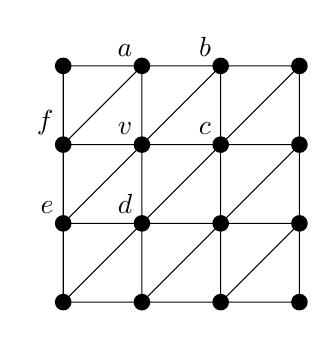
\begin{tikzpicture}
  \draw
    (0, 0) grid[step=1cm] (3, 3)
    (0, 2) -- (1, 3)
    (0, 1) -- (2, 3)
    (0, 0) -- (3, 3)
    (1, 0) -- (3, 2)
    (2, 0) -- (3, 1)
  ;
  \fill[radius=3pt]
    \foreach \x in {0, ..., 3} {
      \foreach \y in {0, ..., 3} {
        (\x, \y) circle[]
      }
    }
  ;
  \path[above left]
    \foreach \p/\v in {
      {1, 3}/a,
      {2, 3}/b,
      {0, 2}/f,
      {1, 2}/v,
      {2, 2}/c,
      {0, 1}/e,
      {1, 1}/d%
    } {
      (\p) node {$\v$}
    }
  ;
\end{tikzpicture}
\caption{The link of \( v \) in this complex consists of the vertices \( \{a,b,c,d,e,f\} \) and the edges \( \{ab,bc,cd,de,ef,fa\} \), forming a hexagon.}
\label{fig:link}
\end{figure}

\begin{mydef}
A \defemph{combinatorial manifold} (or \defemph{combinatorial triangulation}) of dimension \( n \) is a simplicial complex of dimension \( n \) such that the link of every vertex is a simplicial sphere of dimension \( n-1 \) (i.e. its geometric realization is homeomorphic to an \( n-1 \)-sphere). Denote by \( \combmfdset \) the type of combinatorial manifolds of dimension \( n \) (which the notation again reminds us are sets).
\end{mydef}

In a 2-dimensional combinatorial manifold the link is a polygon. See Figures~\ref{fig:sphere_triangulation}, \ref{fig:torus_wiki_triangulation}, and \ref{fig:genus3_wiki_triangulation} for some examples of 2-dimensional combinatorial manifolds of genus 0, 1, and 3.

A classical 1940 result of Whitehead, building on Cairn, states that every smooth manifold admits a combinatorial triangulation\cite{whitehead_triangulation}. So it appears reasonably well motivated to study this class of objects.

\begin{figure}[htbp]
\centering
\includegraphics[width=200pt]{triangulated_sphere.pdf}
\caption{A combinatorial triangulation of a sphere, created with stripy.}
\label{fig:sphere_triangulation}
\end{figure}

\begin{figure}[htbp]
\centering
\includegraphics[width=200pt]{Torus-triang.png}
\caption{A torus with an interesting triangulation, from Wikipedia. The links have various vertex counts from 5-7. Clearly a constant value of 6 would also work. (By Ag2gaeh - Own work, CC BY-SA 3.0, https://commons.wikimedia.org/w/index.php?curid=30856793)}
\label{fig:torus_wiki_triangulation}
\end{figure}

\begin{figure}[htbp]
\centering
\includegraphics[width=200pt]{triangulated_genus3.pdf}
\caption{A 3-holes torus with triangulation, from Wikipedia. (By Ag2gaeh - Own work, CC BY-SA 3.0, https://commons.wikimedia.org/wiki/File:Tri-brezel.svg)}
\label{fig:genus3_wiki_triangulation}
\end{figure}

\subsection{Higher inductive combinatorial manifolds}

To convert a simplicial complex \( M \) of dimension at most 2 to a higher inductive type, we will convert the data in each classical dimension to a path constructor of the corresponding HoTT dimension.

\begin{mydef}
The function \( \mathcal{R}:\simcompt\to\Type \) is called \defemph{realization} and creates a higher inductive type from the data of a simplicial complex. Given \( M:\simcompt \) then \( \mathcal{R}(M) \) is given by
\begin{enumerate}
\item vertices: a function \( \mathsf{v_0}:M_0\to \mathcal{R}(M) \) serving as the 0-dimensional constructors
\item edges: a function \( \mathsf{v_1} \) on 1-faces, sending \( \{a, b\}\mapsto \mathsf{v_0}(a)=\mathsf{v_0}(b) \)
\item 2-faces: a function \( \mathsf{v_2} \) on 2-faces, sending \( \{a, b, c\}\mapsto \refl_a = \mathsf{v_1}(\{a, b\})\cdot \mathsf{v_1}(\{b, c\})\cdot \mathsf{v_1}(\{a, c\})^{-1} \).
\end{enumerate}
\end{mydef}

\subsection{Polygons}\label{sec:polygons}

We will begin with a type that is important both for the domain and the codomain of mere circles: a square.

\begin{mydef}
The higher inductive type \( C_4 \) (where C stands for ``circle'').
\begin{align*}
C_4 &: \Type \\
c_1, c_2, c_3, c_4 &: C_4 \\
c_1c_2 &: c_1 = c_2 \\
c_2c_3 &: c_2 = c_3 \\
c_3c_4 &: c_3 = c_4 \\
c_4c_1 &: c_4 = c_1 \\
\end{align*}
\end{mydef}

\begin{figure}[htbp]
\centering
\begin{tikzpicture}[
node distance = 15mm and 15mm,
V/.style = {circle, fill, draw=black, inner sep=1pt, font=\footnotesize},
every edge quotes/.style = {auto, font=\footnotesize},
arrow/.style={->,semithick}
]
\begin{scope}[nodes=V]
  \node[label=above left:\( c_1 \)] (1) {};
  \node[label=above right:\( c_2 \)] (2) [right=of 1]  {};
  \node[label=below right:\( c_3 \)] (3) [below=of 2]  {};
  \node[label=below left:\( c_4 \)] (4) [below=of 1]  {};
\end{scope}
\draw[arrow]
        (1)  edge["\( c_1c_2 \)"] (2)
        (2)  edge["\( c_2c_3 \)"] (3)
        (3)  edge["\( c_3c_4 \)"] (4)
        (4)  edge["\( c_4c_1 \)"] (1);
\end{tikzpicture}

\caption{The HIT \( C_4 \).}
\end{figure}

The standard HoTT circle itself is a non-example of a combinatorial manifold since it lacks the second vertex of the edge:

\begin{mydef}
The higher inductive type \( \so \):
\begin{align*}
\so &:\Type \\
\mathsf{base}&:\so \\
\mathsf{loop}&:\mathsf{base}=\mathsf{base}
\end{align*}
\end{mydef}

Nonetheless, all polygons are equivalent to each other and to \( \so \).

\begin{mylemma}
The function \( \ell:C_4\to\so \) given by \( \ell(c_i)=\mathsf{base} \) for all \( i \), and \( \ell(c_ic_j)=\mathsf{loop} \) for all \( i,j \) is an equivalence with inverse \( \ell^{-1}(\mathsf{base})=c_1 \) and \( \ell^{-1}(\mathsf{loop})=c_1c_2\cdot c_2c_3\cdot c_3c_4\cdot c_4c_1 \). There are clearly other inverses for different choices of vertex.
\end{mylemma}
\begin{proof}
We can adapt the proof in the HoTT Book\cite{hottbook} of Lemma 6.5.1 which proves that \( \Sigma\mathbf{2}\simeq S^1 \).
\end{proof}

Recalling that terms of \( \EMzo \) are pairs: a type, and a mere equivalence with \( \so \), we have:

\begin{mycor}
We have \( (C_4,||\ell||_{-1}):\EMzo. \)
\end{mycor}

Real-world triangulations of surfaces will often have links whose number of vertices varies across the surface. For example we can see hexagons and pentagons in Figure~\ref{fig:sphere_triangulation}. This presumably introduces only a minor practical inconvenience and doesn't materially affect the discussion to come.

\subsection{\texorpdfstring{The higher inductive type \( \oo \)}{The higher inductive type O}}

We will create our first combinatorial surface, a 2-sphere. We will adopt the convention that a subscript indicates the dimension of a subskeleton of a complex. For instance, we have \( \mathsf{base}:\so_0 \).

\begin{mydef}
The HIT \( \oo_0 \) is just 6 points, intended as the 0-skeleton of an octahedron, with vertices named after the colors on the faces of a famous Central European puzzle cube.
\[ w, y, b, r, g, o : \oo_0 \]
\end{mydef}

\begin{mydef}
The HIT \( \oo_1 \) is the 1-skeleton of an octahedron.
\begin{align*}
w, y, b, r, g, o &: \oo_1 & yg &: y=g \\
wb &: w=b & yo &: y=o \\
wr &: w=r & br &: b=r \\
wg &: w=g & rg &: r=g \\
wo &: w=o & go &: g=o \\
yb &: y=b & ob &: o=b \\
yr &: y=r
\end{align*}
\end{mydef}

\begin{mydef}
The HIT \( \oo \) is an octahedron:
\begin{align*}
w, y, b, r, g, o &: \oo \\
wb &: w=b & br &: b=r & wbr &: wb\cdot br\cdot wr^{-1} = \refl_w \\
wr &: w=r & rg &: r=g & wrg &: wr\cdot rg\cdot wg^{-1} = \refl_w \\
wg &: w=g & go &: g=o & wgo &: wg\cdot go\cdot wo^{-1} = \refl_w \\
wo &: w=o & ob &: o=b & wob &: wo\cdot ob\cdot wb^{-1} = \refl_w \\
yb &: y=b & & & yrb &: yr\cdot rb\cdot yb^{-1} = \refl_y \\
yr &: y=r & & & ygr &: yg\cdot gr\cdot yr^{-1} = \refl_y \\
yg &: y=g & & & yog &: yo\cdot og\cdot yg^{-1} = \refl_y \\
yo &: y=o & & & ybo &: yb\cdot bo\cdot yo^{-1} = \refl_y 
\end{align*}
\end{mydef}

\begin{figure}[htbp]
\centering
\input{discrete_gauge_theory_oo_tikz}
\caption{The HIT \( \oo \) which has 6 points, 12 1-paths, 8 2-paths.}
\end{figure}

We have obvious maps \( \oo_0\xrightarrow[]{i_0} \oo_1\xrightarrow[]{i_1} \oo \) that include each skeleton into the next-higher-dimensional skeleton.

\subsection{Groupoid operations on higher inductive combinatorial manifolds}

Let \( M:\simcompt \) be a combinatorial 2-manifold and \( \mm\defeq\mathcal{R}(M):\combmfdt \) its realization as a higher inductive type. \( \mm \) has triangular 2-faces just as \( M \) does, except they are 2-paths in the HoTT sense. If two faces \( bca \) and \( bdc \) share the edge \( bc \) (see Figure~\ref{fig:concat}), then we can form the type \( bca':ba\cdot ac = bc \) by reorganizing the face as a path from the concatenation of two edges to the third edge. Similarly we can form \( bdc':bd\cdot dc=bc \). We can now concatenate these:
\[ 
bca'\cdot bdc'^{-1}: ba\cdot ac = bd\cdot dc
\] 
which fills the 4-gon \( abdc \), and so can be reorganized as a path \( abdc:\refl_a=\refl_a \) or a path \( bdca:\refl_b=\refl_b \) or other possibilities.
\begin{figure}[htbp]
\centering
\includegraphics[width=200pt]{concat.pdf}
\caption{Concatenating the triangles \( abc \) and \( bdc \) gives the 4-gon \( abdc \).}
\label{fig:concat}
\end{figure}

We will have two use cases for this operation. The first is to consider the concatenation of \emph{all} the faces of \( \mm \), which if we choose a base point \( x:\mm \) is a path from \( \refl_x \) to itself. This will play the role of the ``fundamental homology class'' from classical topology, which is an object on which 2-forms can be evaluated to compute their value on the whole manifold. 

\begin{mydef}
\label{def:totalface}
If \( \mm:\combmfdt \) is a combinatorial manifold and \( v:\mm_0 \) is a vertex, a \( total face \) of \( \mm \) is any concatenation of all the data in \( \mm \) that produces a term in \( \refl_v=\refl_v \).
\end{mydef}

The second use case for concatenating faces is to create an \emph{equivalent} type to \( \mm \) but without one of the point constructors. Figure~\ref{fig:hex_concat} illustrates the equivalence.
\begin{figure}[htbp]
\centering
\includegraphics[width=200pt]{hex_concat.pdf}
\caption{Concatenating the six triangles in the approrpiate way produces a 2-path in \( \refl_v=\refl_v \).}
\label{fig:hex_concat}
\end{figure}

\begin{mydef}
If \( \mm:\combmfdt \) is a combinatorial manifold and \( Z\subset \mm_0 \) is a set of vertices in \( \mm \) with members \( Z=\{z_0,\ldots,z_n\} \), then denote by \( \mm\setminus Z \) the type given by omitting the vertices in \( Z \) from the constructors in all dimensions where they appeared. Call the points of \( Z \) \defemph{isolated} if no two of them are neighbors, i.e. we have \( \pit{z:Z}\link(z)\cap Z=\emptyset \). In the isolated case \( \mm\setminus Z \) has boundary circles where each vertex was removed.
\end{mydef}

\begin{mydef}
\label{def:replacement}
If we have \( \mm\setminus Z \) for some isolated set of verticies \( Z \), then for each \( z:Z \) we can compose all the faces which contain \( z \), forming a new face (see Figure~\ref{fig:hex_concat}). In this way we produce an equivalent type \( \mm_Z\simeq \mm \) but which is no longer combinatorial since we have erased some of the edges from some of the neighborhoods. We call \( \mm_Z \) the \defemph{replacement of \( \mm \) without \( Z \)}.
\end{mydef}

\subsection{The function \texorpdfstring{\( \link \)}{link}}

Taking the link of a vertex gives us a map to polygons.

\begin{mydef}
\( \link:\oo_0\to\EMzo \) is given by:
\begin{align*}
\link(w) &= brgo & \link(r) &= wbyg \\
\link(y) &= bogr & \link(g) &= wryo \\
\link(b) &= woyr & \link(o) &= wgyb
\end{align*}
We chose these orderings for the vertices in the link, by visualizing standing at the given vertex as if it were the north pole, then looking south and enumerating the link in clockwise order, starting from \( w \) if possible, else \( b \).
\end{mydef}

\begin{figure}[htbp]
\centering
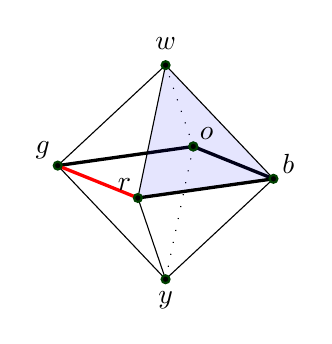
\begin{tikzpicture}%
  [x={(-0.860769cm, -0.121512cm)},
  y={(0.508996cm, -0.205391cm)},
  z={(-0.000053cm, 0.971107cm)},
  scale=1,
  eqback/.style={very thick},
  back/.style={loosely dotted, thin},
  eqedge/.style={very thick},
  edge/.style={black, thin},
  r/.style={red},
  facet/.style={fill=blue!95!black,fill opacity=0.1},
  vertex/.style={inner sep=1pt,circle,draw=green!25!black,fill=black,thick}]
\coordinate (-1, -1, 0) at (-1, -1, 0);
\coordinate (-1, 1, 0) at (-1, 1, 0);
\coordinate (0, 0, -1) at (0, 0, -1);
\coordinate (0, 0, 1) at (0, 0, 1);
\coordinate (1, -1, 0) at (1, -1, 0);
\coordinate (1, 1, 0) at (1, 1, 0);
%% Drawing edges in the back
%%
\draw[edge,eqback] (-1, -1, 0) -- (-1, 1, 0);
\draw[edge,back] (-1, -1, 0) -- (0, 0, -1.4);
\draw[edge,back] (-1, -1, 0) -- (0, 0, 1.4);
\draw[edge,eqback] (1, -1, 0) -- (-1, -1, 0);
%% Drawing vertices in the back
%%
\node[vertex] at (-1, -1, 0)     {};
%% Drawing the facets
%%
%\fill[facet] (1, 1, 0) -- (0, 0, -1.4) -- (1, -1, 0) -- cycle {};
%\fill[facet] (1, 1, 0) -- (0, 0, 1.4) -- (1, -1, 0) -- cycle {};
\fill[facet] (1, 1, 0) -- (-1, 1, 0) -- (0, 0, 1.4) -- cycle {};
%\fill[facet] (1, 1, 0) -- (-1, 1, 0) -- (0, 0, -1.4) -- cycle {};
%% Drawing edges in the front
%%
\draw[edge] (-1, 1, 0) -- (0, 0, -1.4);
\draw[edge] (-1, 1, 0) -- (0, 0, 1.4);
\draw[eqedge] (-1, 1, 0) -- (1, 1, 0);
\draw[edge] (0, 0, -1.4) -- (1, -1, 0);
\draw[edge] (0, 0, -1.4) -- (1, 1, 0);
\draw[edge] (0, 0, 1.4) -- (1, -1, 0);
\draw[edge] (0, 0, 1.4) -- (1, 1, 0);
\draw[r,eqedge] (1, 1, 0) -- (1, -1, 0);
%% Drawing the vertices in the front
%%
\begin{scope}[nodes=vertex]
\node[label=above right:\( b \)] at (-1, 1, 0)     {};
\node[label=below:\( y \)] at (0, 0, -1.4)     {};
\node[label=above:\( w \)] at (0, 0, 1.4)     {};
\node[label=above left:\( g \)] at (1, -1, 0)     {};
\node[label=above left:\( r \)] at (1, 1, 0)     {};
\node[label=above right:\( o \)] at (-1, -1, 0)     {};
\end{scope}
\end{tikzpicture}
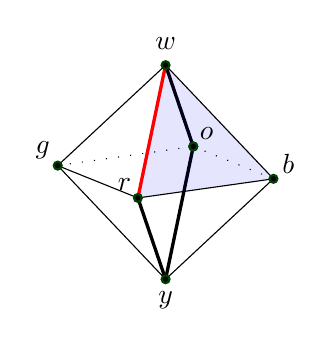
\begin{tikzpicture}%
  [x={(-0.860769cm, -0.121512cm)},
  y={(0.508996cm, -0.205391cm)},
  z={(-0.000053cm, 0.971107cm)},
  scale=1,
  eqback/.style={very thick},
  back/.style={loosely dotted, thin},
  eqedge/.style={very thick},
  r/.style={red},
  edge/.style={black, thin},
  facet/.style={fill=blue!95!black,fill opacity=0.1},
  vertex/.style={inner sep=1pt,circle,draw=green!25!black,fill=black,thick}]
\coordinate (-1, -1, 0) at (-1, -1, 0);
\coordinate (-1, 1, 0) at (-1, 1, 0);
\coordinate (0, 0, -1) at (0, 0, -1);
\coordinate (0, 0, 1) at (0, 0, 1);
\coordinate (1, -1, 0) at (1, -1, 0);
\coordinate (1, 1, 0) at (1, 1, 0);
%% Drawing edges in the back
%%
\draw[edge,back] (-1, -1, 0) -- (-1, 1, 0);
\draw[edge,eqback] (-1, -1, 0) -- (0, 0, -1.4);
\draw[edge,eqback] (0, 0, 1.4) -- (-1, -1, 0);
\draw[edge,back] (1, -1, 0) -- (-1, -1, 0);
%% Drawing vertices in the back
%%
\node[vertex] at (-1, -1, 0)     {};
%% Drawing the facets
%%
% \fill[facet] (1, 1, 0) -- (0, 0, -1.4) -- (1, -1, 0) -- cycle {};
% \fill[facet] (1, 1, 0) -- (0, 0, 1.4) -- (1, -1, 0) -- cycle {};
\fill[facet] (1, 1, 0) -- (-1, 1, 0) -- (0, 0, 1.4) -- cycle {};
% \fill[facet] (1, 1, 0) -- (-1, 1, 0) -- (0, 0, -1.4) -- cycle {};
%% Drawing edges in the front
%%
\draw[edge] (-1, 1, 0) -- (0, 0, -1.4);
\draw[edge] (-1, 1, 0) -- (0, 0, 1.4);
\draw[edge] (-1, 1, 0) -- (1, 1, 0);
\draw[edge] (0, 0, -1.4) -- (1, -1, 0);
\draw[eqedge] (0, 0, -1.4) -- (1, 1, 0);
\draw[edge] (0, 0, 1.4) -- (1, -1, 0);
\draw[r,eqedge] (1, 1, 0) -- (0, 0, 1.4) ;
\draw[edge] (1, 1, 0) -- (1, -1, 0);
%% Drawing the vertices in the front
%%
\begin{scope}[nodes=vertex]
\node[label=above right:\( b \)] at (-1, 1, 0)     {};
\node[label=below:\( y \)] at (0, 0, -1.4)     {};
\node[label=above:\( w \)] at (0, 0, 1.4)     {};
\node[label=above left:\( g \)] at (1, -1, 0)     {};
\node[label=above left:\( r \)] at (1, 1, 0)     {};
\node[label=above right:\( o \)] at (-1, -1, 0)     {};
\end{scope}
\end{tikzpicture}
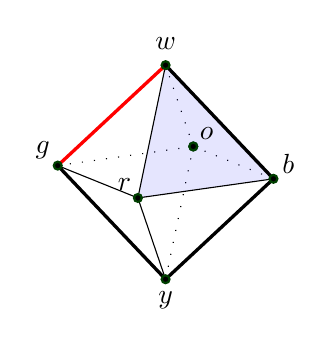
\begin{tikzpicture}%
  [x={(-0.860769cm, -0.121512cm)},
  y={(0.508996cm, -0.205391cm)},
  z={(-0.000053cm, 0.971107cm)},
  scale=1,
  eqback/.style={very thick},
  back/.style={loosely dotted, thin},
  eqedge/.style={very thick},
  r/.style={red},
  edge/.style={black, thin},
  facet/.style={fill=blue!95!black,fill opacity=0.1},
  vertex/.style={inner sep=1pt,circle,draw=green!25!black,fill=black,thick}]
\coordinate (-1, -1, 0) at (-1, -1, 0);
\coordinate (-1, 1, 0) at (-1, 1, 0);
\coordinate (0, 0, -1) at (0, 0, -1);
\coordinate (0, 0, 1) at (0, 0, 1);
\coordinate (1, -1, 0) at (1, -1, 0);
\coordinate (1, 1, 0) at (1, 1, 0);
%% Drawing edges in the back
%%
\draw[edge,back] (-1, -1, 0) -- (-1, 1, 0);
\draw[edge,back] (-1, -1, 0) -- (0, 0, -1.4);
\draw[edge,back] (-1, -1, 0) -- (0, 0, 1.4);
\draw[edge,back] (1, -1, 0) -- (-1, -1, 0);
%% Drawing vertices in the back
%%
\node[vertex] at (-1, -1, 0)     {};
%% Drawing the facets
%%
% \fill[facet] (1, 1, 0) -- (0, 0, -1.4) -- (1, -1, 0) -- cycle {};
% \fill[facet] (1, 1, 0) -- (0, 0, 1.4) -- (1, -1, 0) -- cycle {};
\fill[facet] (1, 1, 0) -- (-1, 1, 0) -- (0, 0, 1.4) -- cycle {};
% \fill[facet] (1, 1, 0) -- (-1, 1, 0) -- (0, 0, -1.4) -- cycle {};
%% Drawing edges in the front
%%
\draw[eqedge] (-1, 1, 0) -- (0, 0, -1.4);
\draw[eqedge] (0, 0, 1.4) -- (-1, 1, 0);
\draw[edge] (-1, 1, 0) -- (1, 1, 0);
\draw[eqedge] (0, 0, -1.4) -- (1, -1, 0);
\draw[edge] (0, 0, -1.4) -- (1, 1, 0);
\draw[r,eqedge] (1, -1, 0) -- (0, 0, 1.4);
\draw[edge] (0, 0, 1.4) -- (1, 1, 0);
\draw[edge] (1, 1, 0) -- (1, -1, 0);
%% Drawing the vertices in the front
%%
\begin{scope}[nodes=vertex]
\node[label=above right:\( b \)] at (-1, 1, 0)     {};
\node[label=below:\( y \)] at (0, 0, -1.4)     {};
\node[label=above:\( w \)] at (0, 0, 1.4)     {};
\node[label=above left:\( g \)] at (1, -1, 0)     {};
\node[label=above left:\( r \)] at (1, 1, 0)     {};
\node[label=above right:\( o \)] at (-1, -1, 0)     {};
\end{scope}
\end{tikzpicture}
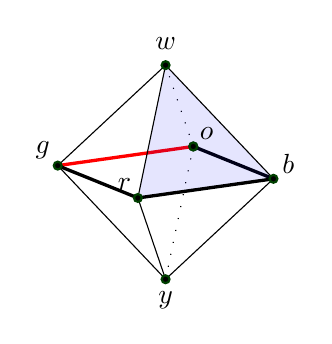
\begin{tikzpicture}%
  [x={(-0.860769cm, -0.121512cm)},
  y={(0.508996cm, -0.205391cm)},
  z={(-0.000053cm, 0.971107cm)},
  scale=1,
  eqback/.style={very thick},
  back/.style={loosely dotted, thin},
  eqedge/.style={very thick},
  edge/.style={black, thin},
  r/.style={red},
  facet/.style={fill=blue!95!black,fill opacity=0.1},
  vertex/.style={inner sep=1pt,circle,draw=green!25!black,fill=black,thick}]
\coordinate (-1, -1, 0) at (-1, -1, 0);
\coordinate (-1, 1, 0) at (-1, 1, 0);
\coordinate (0, 0, -1) at (0, 0, -1);
\coordinate (0, 0, 1) at (0, 0, 1);
\coordinate (1, -1, 0) at (1, -1, 0);
\coordinate (1, 1, 0) at (1, 1, 0);
%% Drawing edges in the back
%%
\draw[edge,eqback] (-1, -1, 0) -- (-1, 1, 0);
\draw[edge,back] (-1, -1, 0) -- (0, 0, -1.4);
\draw[edge,back] (-1, -1, 0) -- (0, 0, 1.4);
\draw[edge,eqback,r] (1, -1, 0) -- (-1, -1, 0);
%% Drawing vertices in the back
%%
\node[vertex] at (-1, -1, 0)     {};
%% Drawing the facets
%%
% \fill[facet] (1, 1, 0) -- (0, 0, -1.4) -- (1, -1, 0) -- cycle {};
% \fill[facet] (1, 1, 0) -- (0, 0, 1.4) -- (1, -1, 0) -- cycle {};
\fill[facet] (1, 1, 0) -- (-1, 1, 0) -- (0, 0, 1.4) -- cycle {};
% \fill[facet] (1, 1, 0) -- (-1, 1, 0) -- (0, 0, -1.4) -- cycle {};
%% Drawing edges in the front
%%
\draw[edge] (-1, 1, 0) -- (0, 0, -1.4);
\draw[edge] (-1, 1, 0) -- (0, 0, 1.4);
\draw[eqedge] (-1, 1, 0) -- (1, 1, 0);
\draw[edge] (0, 0, -1.4) -- (1, -1, 0);
\draw[edge] (0, 0, -1.4) -- (1, 1, 0);
\draw[edge] (0, 0, 1.4) -- (1, -1, 0);
\draw[edge] (0, 0, 1.4) -- (1, 1, 0);
\draw[eqedge] (1, 1, 0) -- (1, -1, 0);
%% Drawing the vertices in the front
%%
\begin{scope}[nodes=vertex]
\node[label=above right:\( b \)] at (-1, 1, 0)     {};
\node[label=below:\( y \)] at (0, 0, -1.4)     {};
\node[label=above:\( w \)] at (0, 0, 1.4)     {};
\node[label=above left:\( g \)] at (1, -1, 0)     {};
\node[label=above left:\( r \)] at (1, 1, 0)     {};
\node[label=above right:\( o \)] at (-1, -1, 0)     {};
\end{scope}
\end{tikzpicture}

\caption{\( \link \) for the verticies \( w, b\) and \( r \).}
\label{fig:triangle_of_equators}
\end{figure}

To extend \( \link \) to the 1-skeleton we have complete freedom. We will do something ``tangent bundley'', imagining how \( \link \) changes as we slide from point to point in the embedding shown in the figures. Sliding from \( w \) to \( b \) and tipping the link as we go, we see \( r\mapsto r \) and \( o\mapsto o \) because those lie on the axis of rotation. Then \( g\mapsto w \) and \( b\mapsto y \). 

\begin{mydef}
Define \( T_1:\oo_1\to\EMzo \) on just the 1-skeleton by extending \( \link \) as follows:
Transport away from \( w \):
\begin{itemize}
\item \( T_1(wb):[b, r, g, o]\mapsto [y, r, w, o] \) (\( r, o \) fixed)
\item \( T_1(wr):[b, r, g, o]\mapsto [b, y, g, w] \) (\( b, g \) fixed)
\item \( T_1(wg):[b, r, g, o]\mapsto [w, r, y, o] \)
\item \( T_1(wo):[b, r, g, o]\mapsto [b, w, g, y] \)
\end{itemize}
Transport away from \( y \):
\begin{itemize}
\item \( T_1(yb):[b, o, g, r]\mapsto [w, o, y, r] \)
\item \( T_1(yr):[b, o, g, r]\mapsto [b, y, g, w] \)
\item \( T_1(yg):[b, o, g, r]\mapsto [y, o, w, r] \)
\item \( T_1(yo):[b, o, g, r]\mapsto [b, w, g, y] \)
\end{itemize}
Transport along the equator:
\begin{itemize}
\item \( T_1(br):[w, o, y, r]\mapsto [w, b, y, g] \) 
\item \( T_1(rg):[w, b, y, g]\mapsto [w, r, y, o] \)
\item \( T_1(go):[w, r, y, o]\mapsto [w, g, y, b] \)
\item \( T_1(ob):[w, g, y, b]\mapsto [w, o, y, r] \)
\end{itemize}
\end{mydef}

It's very important to be able to visualize what \( T_1 \) does to triangular paths such as \( wb\cdot br\cdot rw \) (which circulates around the boundary of face \( wbr \)). You can see it if you imagine Figure~\ref{fig:triangle_of_equators} as the frames of a short movie. Or you can place your palm over the top of a cube and note where your fingers are pointing, then slide your hand to an equatorial face, then along the equator, then back to the top. The answer is: you come back rotated clockwise by a quarter-turn. 

\begin{mydef}
The map \( R:C_4\to C_4 \) rotates by one quarter turn, one ``click":
\begin{multicols}{2}
\begin{itemize}
\item \( R(c_1) = c_2 \)
\item \( R(c_2) = c_3 \)
\item \( R(c_3) = c_4 \)
\item \( R(c_4) = c_1 \)
\item \( R(c_1c_2) = c_2c_3 \)
\item \( R(c_2c_3) = c_3c_4 \)
\item \( R(c_3c_4) = c_4c_1 \)
\item \( R(c_4c_1) = c_1c_2 \)
\end{itemize}
\end{multicols}
\end{mydef}

Now let's extend \( T_1 \) to all of \( \oo \) by providing values for the eight faces. The face \( wbr \) is a path from \( \refl_w \) to the concatenation \( wb\cdot br\cdot rw \), and so the image of \( wbr \) under the extended version of \( T_1 \) must be a homotopy from \( \refl_{T_1(w)} \) to \( T_1(wb\cdot br\cdot rw) \). Here there is no additional freedom.

\begin{mydef}
Define \( T_2:\oo\to\EMzo \) by extending \( T_1 \) to the faces as follows:
\begin{multicols}{2}
\begin{itemize}
\item \( T_2(wbr)=H_R \) 
\item \( T_2(wrg)=H_R \)
\item \( T_2(wgo)=H_R \)
\item \( T_2(ybo)=H_R \)
\item \( T_2(yrb)=H_R \) 
\item \( T_2(ygr)=H_R \)
\item \( T_2(yog)=H_R \)
\item \( T_2(ybo)=H_R \)
\end{itemize}
\end{multicols}
where \( H_R:R=\refl \) is the obvious homotopy.
\end{mydef}

All the faces do the same thing: they map to a homotopy between the identity and clockwise rotation by a quarter turn. Concatenating the eight faces in the 2-groupoid \( \oo \) would then map to a homotopy between the identity and two full rotations. This makes visible in HoTT the link between curvature and the Euler characteristic (which is 2 for the octahedron). More on that later.

\subsection{The torus}

We can define a combinatorial torus as a similar HIT. This time each vertex will have six neighbors. So all the links will be merely equal to \( C_6 \) which is a hexagonal version of \( C_4 \). See Figure~\ref{fig:torus}. 

To help parse this figure, imagine instead Figure~\ref{fig:flattorus}. We take this simple alternating-triangle pattern, then glue the left and right edges, then bend into Figure~\ref{fig:torus}. The fact that each column in Figure~\ref{fig:flattorus} has four dots corresponds to the torus in Figure~\ref{fig:torus} having a square in front, diamonds in the middle, and a square in back.

\begin{figure}[htbp]
\centering
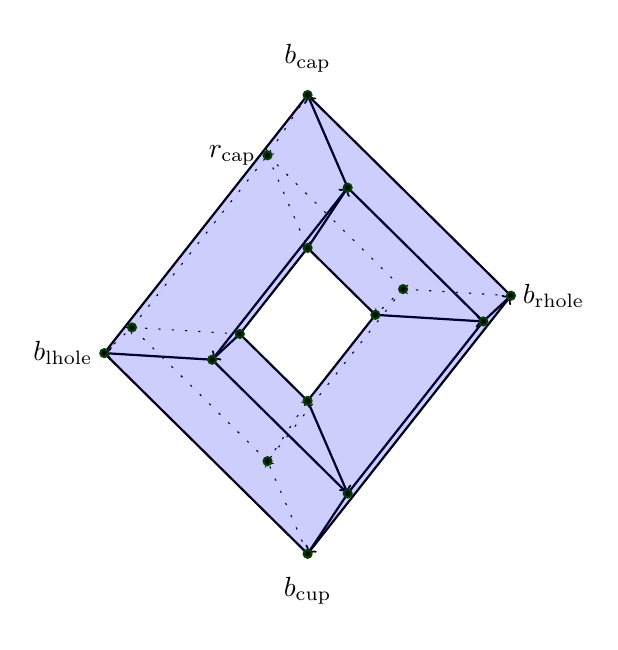
\begin{tikzpicture}%
  [x={(-0.860769cm, -0.121512cm)},
  y={(0.508996cm, -0.205391cm)},
  z={(-0.000053cm, 0.971107cm)},
  scale=1,
  back/.style={loosely dotted, thin},
  edge/.style={->,black, thick},
  line/.style={black, thick},
  facet/.style={fill=blue!95!black,fill opacity=0.1},
  vertex/.style={inner sep=1pt,circle,draw=green!25!black,fill=black,thick}]
\coordinate (r_cap) at (0, -1, 5);
\coordinate (g_cap) at (0, 0, 4 );
\coordinate (o_cap) at (0, 1, 5 );
\coordinate (b_cap) at (0, 0, 6 );

\coordinate (r_cup) at (0, -1, 1);
\coordinate (g_cup) at (0, 0, 2 );
\coordinate (o_cup) at (0, 1, 1 );
\coordinate (b_cup) at (0, 0, 0 );

\coordinate (r_ohole) at (-2, -1, 3);
\coordinate (g_ohole) at (-1, 0,  3);
\coordinate (o_ohole) at (-2, 1,  3);
\coordinate (b_ohole) at (-3, 0,  3);

\coordinate (r_rhole) at (2, -1, 3);
\coordinate (g_rhole) at (1, 0,  3);
\coordinate (o_rhole) at (2, 1,  3);
\coordinate (b_rhole) at (3, 0,  3);

\draw[edge,back] (r_cap) -- (g_cap);
\draw[edge]      (g_cap) -- (o_cap);
\draw[edge]      (o_cap) -- (b_cap);
\draw[edge,back] (b_cap) -- (r_cap);

\draw[edge,back] (r_cup) -- (g_cup);
\draw[edge]      (g_cup) -- (o_cup);
\draw[edge]      (o_cup) -- (b_cup);
\draw[edge,back] (b_cup) -- (r_cup);

\draw[edge,back] (r_ohole) -- (g_ohole);
\draw[edge]      (g_ohole) -- (o_ohole);
\draw[edge]      (o_ohole) -- (b_ohole);
\draw[edge,back] (b_ohole) -- (r_ohole);

\draw[edge,back] (r_rhole) -- (g_rhole);
\draw[edge]      (g_rhole) -- (o_rhole);
\draw[edge]      (o_rhole) -- (b_rhole);
\draw[edge,back] (b_rhole) -- (r_rhole);

\draw[line,back] (r_cap) --   (r_ohole);
\draw[line,back] (r_ohole) -- (r_cup);
\draw[line,back] (r_cup) --   (r_rhole);
\draw[line,back] (r_rhole) -- (r_cap);

\draw[line] (g_cap) --   (g_ohole);
\draw[line] (g_ohole) -- (g_cup);
\draw[line] (g_cup) --   (g_rhole);
\draw[line] (g_rhole) -- (g_cap);

\draw[line] (o_cap) --   (o_ohole);
\draw[line] (o_ohole) -- (o_cup);
\draw[line] (o_cup) --   (o_rhole);
\draw[line] (o_rhole) -- (o_cap);

\draw[line] (b_cap) --   (b_ohole);
\draw[line] (b_ohole) -- (b_cup);
\draw[line] (b_cup) --   (b_rhole);
\draw[line] (b_rhole) -- (b_cap);

\fill[facet] (r_cap) -- (r_ohole) -- (g_ohole) -- (g_cap) -- cycle {};
\fill[facet] (r_cap) -- (r_rhole) -- (g_rhole) -- (g_cap) -- cycle {};
\fill[facet] (r_cap) -- (r_ohole) -- (b_ohole) -- (b_cap) -- cycle {};
\fill[facet] (r_cap) -- (r_rhole) -- (b_rhole) -- (b_cap) -- cycle {};

\fill[facet] (o_cap) -- (o_ohole) -- (g_ohole) -- (g_cap) -- cycle {};
\fill[facet] (o_cap) -- (o_rhole) -- (g_rhole) -- (g_cap) -- cycle {};
\fill[facet] (o_cap) -- (o_ohole) -- (b_ohole) -- (b_cap) -- cycle {};
\fill[facet] (o_cap) -- (o_rhole) -- (b_rhole) -- (b_cap) -- cycle {};

\fill[facet] (r_cup) -- (r_ohole) -- (g_ohole) -- (g_cup) -- cycle {};
\fill[facet] (r_cup) -- (r_rhole) -- (g_rhole) -- (g_cup) -- cycle {};
\fill[facet] (r_cup) -- (r_ohole) -- (b_ohole) -- (b_cup) -- cycle {};
\fill[facet] (r_cup) -- (r_rhole) -- (b_rhole) -- (b_cup) -- cycle {};

\fill[facet] (o_cup) -- (o_ohole) -- (g_ohole) -- (g_cup) -- cycle {};
\fill[facet] (o_cup) -- (o_rhole) -- (g_rhole) -- (g_cup) -- cycle {};
\fill[facet] (o_cup) -- (o_ohole) -- (b_ohole) -- (b_cup) -- cycle {};
\fill[facet] (o_cup) -- (o_rhole) -- (b_rhole) -- (b_cup) -- cycle {};

\begin{scope}[nodes=vertex]
\node[label=left:\( r_{\mathrm{cap}} \)] at (r_cap) {};
\node at (g_cap) {};
\node at (o_cap) {};
\node[label=above:\( b_{\mathrm{cap}} \)] at (b_cap) {};
\node at (r_cup) {};
\node at (g_cup) {};
\node at (o_cup) {};
\node[label=below:\( b_{\mathrm{cup}} \)] at (b_cup) {};
\node at (r_ohole) {};
\node at (g_ohole) {};
\node at (o_ohole) {};
\node[label=right:\( b_{\mathrm{rhole}} \)] at (b_ohole) {};
\node at (r_rhole) {};
\node at (g_rhole) {};
\node at (o_rhole) {};
\node[label=left:\( b_{\mathrm{lhole}} \)] at (b_rhole) {};
\end{scope}
\end{tikzpicture}

\caption{Torus embedded in 3-dimensional space. If you see color in your rendering then black lines trace four square-shaped paths, red ones connect the front square to the middle diamonds, and blue ones connect the back path to the middle ones.}
\label{fig:torus}
\end{figure}

\begin{figure}[htbp]
\centering
% https://q.uiver.app/#q=WzAsMzYsWzEsNCwiXFxidWxsZXQiXSxbMSw2LCJcXGJ1bGxldCJdLFsyLDcsIlxcYnVsbGV0Il0sWzIsNSwiXFxidWxsZXQiXSxbMiwzLCJcXGJ1bGxldCJdLFsxLDgsIlxcYnVsbGV0Il0sWzEsMiwiXFxidWxsZXQiXSxbMywyLCJcXGJ1bGxldCJdLFszLDQsIlxcYnVsbGV0Il0sWzMsNiwiXFxidWxsZXQiXSxbMyw4LCJcXGJ1bGxldCJdLFsyLDEsIlxcYnVsbGV0Il0sWzQsMSwiXFxidWxsZXQiXSxbNSwyLCJcXGJ1bGxldCJdLFs0LDMsIlxcYnVsbGV0Il0sWzUsNCwiXFxidWxsZXQiXSxbNCw1LCJcXGJ1bGxldCJdLFs1LDYsIlxcYnVsbGV0Il0sWzQsNywiXFxidWxsZXQiXSxbNSw4LCJcXGJ1bGxldCJdLFsyLDAsIlxcbWF0aHJte2JhY2t9Il0sWzQsMCwiXFxtYXRocm17ZnJvbnR9Il0sWzEsMCwiXFxtYXRocm17b3V0ZXJ9Il0sWzMsMCwiXFxtYXRocm17aG9sZX0iXSxbNSwwLCJcXG1hdGhybXtvdXRlcn0iXSxbMSwxMCwiXFxidWxsZXQiXSxbMiw5LCJcXGJ1bGxldCJdLFszLDEwLCJcXGJ1bGxldCJdLFs0LDksIlxcYnVsbGV0Il0sWzUsMTAsIlxcYnVsbGV0Il0sWzAsMiwiXFxtYXRocm17dG9wXFwgb2ZcXCBkaWFtb25kc30iXSxbMCw2LCJcXG1hdGhybXtib3R0b21cXCBvZlxcIGRpYW1vbmRzfSJdLFsxLDEsIlxcICJdLFs1LDEsIlxcICJdLFszLDEsIlxcICJdLFswLDEwLCJcXG1hdGhybXt0b3BcXCBvZlxcIGRpYW1vbmRzfSJdLFs0LDMsIiIsMix7InN0eWxlIjp7ImhlYWQiOnsibmFtZSI6Im5vbmUifX19XSxbMywyLCIiLDIseyJzdHlsZSI6eyJoZWFkIjp7Im5hbWUiOiJub25lIn19fV0sWzAsMSwiIiwyLHsic3R5bGUiOnsiaGVhZCI6eyJuYW1lIjoibm9uZSJ9fX1dLFs0LDAsIiIsMSx7ImNvbG91ciI6WzIzNiw5MSw2MF0sInN0eWxlIjp7ImhlYWQiOnsibmFtZSI6Im5vbmUifX19XSxbMCwzLCIiLDEseyJjb2xvdXIiOlsyMzYsOTEsNjBdLCJzdHlsZSI6eyJoZWFkIjp7Im5hbWUiOiJub25lIn19fV0sWzMsMSwiIiwxLHsiY29sb3VyIjpbMjM2LDkxLDYwXSwic3R5bGUiOnsiaGVhZCI6eyJuYW1lIjoibm9uZSJ9fX1dLFsxLDIsIiIsMSx7ImNvbG91ciI6WzIzNiw5MSw2MF0sInN0eWxlIjp7ImhlYWQiOnsibmFtZSI6Im5vbmUifX19XSxbMiw1LCIiLDEseyJjb2xvdXIiOlsyMzYsOTEsNjBdLCJzdHlsZSI6eyJoZWFkIjp7Im5hbWUiOiJub25lIn19fV0sWzEsNSwiIiwxLHsic3R5bGUiOnsiaGVhZCI6eyJuYW1lIjoibm9uZSJ9fX1dLFs2LDQsIiIsMSx7ImNvbG91ciI6WzIzNiw5MSw2MF0sInN0eWxlIjp7ImhlYWQiOnsibmFtZSI6Im5vbmUifX19XSxbNiwwLCIiLDEseyJzdHlsZSI6eyJoZWFkIjp7Im5hbWUiOiJub25lIn19fV0sWzcsOCwiIiwwLHsic3R5bGUiOnsiaGVhZCI6eyJuYW1lIjoibm9uZSJ9fX1dLFs4LDksIiIsMCx7InN0eWxlIjp7ImhlYWQiOnsibmFtZSI6Im5vbmUifX19XSxbOSwxMCwiIiwwLHsic3R5bGUiOnsiaGVhZCI6eyJuYW1lIjoibm9uZSJ9fX1dLFs3LDQsIiIsMCx7ImNvbG91ciI6WzIzNiw5MSw2MF0sInN0eWxlIjp7ImhlYWQiOnsibmFtZSI6Im5vbmUifX19XSxbNCw4LCIiLDAseyJjb2xvdXIiOlsyMzYsOTEsNjBdLCJzdHlsZSI6eyJoZWFkIjp7Im5hbWUiOiJub25lIn19fV0sWzgsMywiIiwwLHsiY29sb3VyIjpbMjM2LDkxLDYwXSwic3R5bGUiOnsiaGVhZCI6eyJuYW1lIjoibm9uZSJ9fX1dLFszLDksIiIsMCx7ImNvbG91ciI6WzIzNiw5MSw2MF0sInN0eWxlIjp7ImhlYWQiOnsibmFtZSI6Im5vbmUifX19XSxbOSwyLCIiLDAseyJjb2xvdXIiOlsyMzYsOTEsNjBdLCJzdHlsZSI6eyJoZWFkIjp7Im5hbWUiOiJub25lIn19fV0sWzIsMTAsIiIsMCx7ImNvbG91ciI6WzIzNiw5MSw2MF0sInN0eWxlIjp7ImhlYWQiOnsibmFtZSI6Im5vbmUifX19XSxbMTEsNCwiIiwwLHsic3R5bGUiOnsiaGVhZCI6eyJuYW1lIjoibm9uZSJ9fX1dLFsxMSw2LCIiLDAseyJjb2xvdXIiOlsyMzYsOTEsNjBdLCJzdHlsZSI6eyJoZWFkIjp7Im5hbWUiOiJub25lIn19fV0sWzExLDcsIiIsMCx7ImNvbG91ciI6WzIzNiw5MSw2MF0sInN0eWxlIjp7ImhlYWQiOnsibmFtZSI6Im5vbmUifX19XSxbMTksMTcsIiIsMCx7InN0eWxlIjp7ImhlYWQiOnsibmFtZSI6Im5vbmUifX19XSxbMTgsMTYsIiIsMCx7InN0eWxlIjp7ImhlYWQiOnsibmFtZSI6Im5vbmUifX19XSxbMTYsMTQsIiIsMCx7InN0eWxlIjp7ImhlYWQiOnsibmFtZSI6Im5vbmUifX19XSxbMTcsMTUsIiIsMCx7InN0eWxlIjp7ImhlYWQiOnsibmFtZSI6Im5vbmUifX19XSxbMTUsMTMsIiIsMCx7InN0eWxlIjp7ImhlYWQiOnsibmFtZSI6Im5vbmUifX19XSxbMTQsMTIsIiIsMCx7InN0eWxlIjp7ImhlYWQiOnsibmFtZSI6Im5vbmUifX19XSxbMTIsNywiIiwwLHsiY29sb3VyIjpbMSw5NSw2MF0sInN0eWxlIjp7ImhlYWQiOnsibmFtZSI6Im5vbmUifX19XSxbMTIsMTMsIiIsMCx7ImNvbG91ciI6WzEsOTUsNjBdLCJzdHlsZSI6eyJoZWFkIjp7Im5hbWUiOiJub25lIn19fV0sWzEzLDE0LCIiLDAseyJjb2xvdXIiOlsxLDk1LDYwXSwic3R5bGUiOnsiaGVhZCI6eyJuYW1lIjoibm9uZSJ9fX1dLFsxNCw4LCIiLDAseyJjb2xvdXIiOlsxLDk1LDYwXSwic3R5bGUiOnsiaGVhZCI6eyJuYW1lIjoibm9uZSJ9fX1dLFsxNCwxNSwiIiwwLHsiY29sb3VyIjpbMSw5NSw2MF0sInN0eWxlIjp7ImhlYWQiOnsibmFtZSI6Im5vbmUifX19XSxbMTUsMTYsIiIsMCx7ImNvbG91ciI6WzEsOTUsNjBdLCJzdHlsZSI6eyJoZWFkIjp7Im5hbWUiOiJub25lIn19fV0sWzgsMTYsIiIsMCx7ImNvbG91ciI6WzEsOTUsNjBdLCJzdHlsZSI6eyJoZWFkIjp7Im5hbWUiOiJub25lIn19fV0sWzE2LDksIiIsMCx7ImNvbG91ciI6WzEsOTUsNjBdLCJzdHlsZSI6eyJoZWFkIjp7Im5hbWUiOiJub25lIn19fV0sWzE2LDE3LCIiLDAseyJjb2xvdXIiOlsxLDk1LDYwXSwic3R5bGUiOnsiaGVhZCI6eyJuYW1lIjoibm9uZSJ9fX1dLFsxNywxOCwiIiwwLHsiY29sb3VyIjpbMSw5NSw2MF0sInN0eWxlIjp7ImhlYWQiOnsibmFtZSI6Im5vbmUifX19XSxbOSwxOCwiIiwwLHsiY29sb3VyIjpbMSw5NSw2MF0sInN0eWxlIjp7ImhlYWQiOnsibmFtZSI6Im5vbmUifX19XSxbMTgsMTksIiIsMCx7ImNvbG91ciI6WzEsOTUsNjBdLCJzdHlsZSI6eyJoZWFkIjp7Im5hbWUiOiJub25lIn19fV0sWzE4LDEwLCIiLDAseyJjb2xvdXIiOlsxLDk1LDYwXSwic3R5bGUiOnsiaGVhZCI6eyJuYW1lIjoibm9uZSJ9fX1dLFs3LDE0LCIiLDAseyJjb2xvdXIiOlsxLDk1LDYwXSwic3R5bGUiOnsiaGVhZCI6eyJuYW1lIjoibm9uZSJ9fX1dLFs1LDI2LCIiLDEseyJjb2xvdXIiOlsyMzYsOTEsNjBdLCJzdHlsZSI6eyJoZWFkIjp7Im5hbWUiOiJub25lIn19fV0sWzEwLDI2LCIiLDEseyJjb2xvdXIiOlsyMzYsOTEsNjBdLCJzdHlsZSI6eyJoZWFkIjp7Im5hbWUiOiJub25lIn19fV0sWzIsMjYsIiIsMSx7InN0eWxlIjp7ImhlYWQiOnsibmFtZSI6Im5vbmUifX19XSxbMTgsMjgsIiIsMSx7InN0eWxlIjp7ImhlYWQiOnsibmFtZSI6Im5vbmUifX19XSxbMjYsMjUsIiIsMSx7ImNvbG91ciI6WzIzNiw5MSw2MF0sInN0eWxlIjp7ImhlYWQiOnsibmFtZSI6Im5vbmUifX19XSxbMjYsMjcsIiIsMSx7ImNvbG91ciI6WzIzNiw5MSw2MF0sInN0eWxlIjp7ImhlYWQiOnsibmFtZSI6Im5vbmUifX19XSxbMjgsMjksIiIsMSx7ImNvbG91ciI6WzEsOTUsNjBdLCJzdHlsZSI6eyJoZWFkIjp7Im5hbWUiOiJub25lIn19fV0sWzE5LDI5LCIiLDEseyJzdHlsZSI6eyJoZWFkIjp7Im5hbWUiOiJub25lIn19fV0sWzEwLDI3LCIiLDEseyJzdHlsZSI6eyJoZWFkIjp7Im5hbWUiOiJub25lIn19fV0sWzUsMjUsIiIsMSx7InN0eWxlIjp7ImhlYWQiOnsibmFtZSI6Im5vbmUifX19XSxbMjgsMjcsIiIsMSx7ImNvbG91ciI6WzEsOTUsNjBdLCJzdHlsZSI6eyJoZWFkIjp7Im5hbWUiOiJub25lIn19fV0sWzI4LDE5LCIiLDEseyJjb2xvdXIiOlsxLDk1LDYwXSwic3R5bGUiOnsiaGVhZCI6eyJuYW1lIjoibm9uZSJ9fX1dLFsyOCwxMCwiIiwxLHsiY29sb3VyIjpbMSw5NSw2MF0sInN0eWxlIjp7ImhlYWQiOnsibmFtZSI6Im5vbmUifX19XSxbMzAsNiwiIiwxLHsic3R5bGUiOnsiYm9keSI6eyJuYW1lIjoiZG90dGVkIn19fV0sWzMxLDEsIiIsMSx7InN0eWxlIjp7ImJvZHkiOnsibmFtZSI6ImRvdHRlZCJ9fX1dLFsyMCwxMSwiIiwwLHsic3R5bGUiOnsiYm9keSI6eyJuYW1lIjoiZG90dGVkIn19fV0sWzIxLDEyLCIiLDAseyJzdHlsZSI6eyJib2R5Ijp7Im5hbWUiOiJkb3R0ZWQifX19XSxbMjIsMzIsIiIsMCx7InN0eWxlIjp7ImJvZHkiOnsibmFtZSI6ImRvdHRlZCJ9fX1dLFsyNCwzMywiIiwwLHsic3R5bGUiOnsiYm9keSI6eyJuYW1lIjoiZG90dGVkIn19fV0sWzIzLDM0LCIiLDAseyJzdHlsZSI6eyJib2R5Ijp7Im5hbWUiOiJkb3R0ZWQifX19XSxbMzUsMjUsIiIsMSx7InN0eWxlIjp7ImJvZHkiOnsibmFtZSI6ImRvdHRlZCJ9fX1dXQ==
\begin{tikzcd}[column sep=1ex,row sep=1ex]
	& {\mathrm{outer}} & {\mathrm{back}} & {\mathrm{hole}} & {\mathrm{front}} & {\mathrm{outer}} \\
	& {\ } & \bullet & {\ } & \bullet & {\ } \\
	{\mathrm{top\ of\ diamonds}} & \bullet && \bullet && \bullet \\
	&& \bullet && \bullet \\
	& \bullet && \bullet && \bullet \\
	&& \bullet && \bullet \\
	{\mathrm{bottom\ of\ diamonds}} & \bullet && \bullet && \bullet \\
	&& \bullet && \bullet \\
	& \bullet && \bullet && \bullet \\
	&& \bullet && \bullet \\
	{\mathrm{top\ of\ diamonds}} & \bullet && \bullet && \bullet
	\arrow[dotted, from=1-2, to=2-2]
	\arrow[dotted, from=1-3, to=2-3]
	\arrow[dotted, from=1-4, to=2-4]
	\arrow[dotted, from=1-5, to=2-5]
	\arrow[dotted, from=1-6, to=2-6]
	\arrow[draw={rgb,255:red,60;green,73;blue,246}, no head, from=2-3, to=3-2]
	\arrow[draw={rgb,255:red,60;green,73;blue,246}, no head, from=2-3, to=3-4]
	\arrow[no head, from=2-3, to=4-3]
	\arrow[draw={rgb,255:red,250;green,59;blue,56}, no head, from=2-5, to=3-4]
	\arrow[draw={rgb,255:red,250;green,59;blue,56}, no head, from=2-5, to=3-6]
	\arrow[dotted, from=3-1, to=3-2]
	\arrow[draw={rgb,255:red,60;green,73;blue,246}, no head, from=3-2, to=4-3]
	\arrow[no head, from=3-2, to=5-2]
	\arrow[draw={rgb,255:red,60;green,73;blue,246}, no head, from=3-4, to=4-3]
	\arrow[draw={rgb,255:red,250;green,59;blue,56}, no head, from=3-4, to=4-5]
	\arrow[no head, from=3-4, to=5-4]
	\arrow[draw={rgb,255:red,250;green,59;blue,56}, no head, from=3-6, to=4-5]
	\arrow[draw={rgb,255:red,60;green,73;blue,246}, no head, from=4-3, to=5-2]
	\arrow[draw={rgb,255:red,60;green,73;blue,246}, no head, from=4-3, to=5-4]
	\arrow[no head, from=4-3, to=6-3]
	\arrow[no head, from=4-5, to=2-5]
	\arrow[draw={rgb,255:red,250;green,59;blue,56}, no head, from=4-5, to=5-4]
	\arrow[draw={rgb,255:red,250;green,59;blue,56}, no head, from=4-5, to=5-6]
	\arrow[draw={rgb,255:red,60;green,73;blue,246}, no head, from=5-2, to=6-3]
	\arrow[no head, from=5-2, to=7-2]
	\arrow[draw={rgb,255:red,60;green,73;blue,246}, no head, from=5-4, to=6-3]
	\arrow[draw={rgb,255:red,250;green,59;blue,56}, no head, from=5-4, to=6-5]
	\arrow[no head, from=5-4, to=7-4]
	\arrow[no head, from=5-6, to=3-6]
	\arrow[draw={rgb,255:red,250;green,59;blue,56}, no head, from=5-6, to=6-5]
	\arrow[draw={rgb,255:red,60;green,73;blue,246}, no head, from=6-3, to=7-2]
	\arrow[draw={rgb,255:red,60;green,73;blue,246}, no head, from=6-3, to=7-4]
	\arrow[no head, from=6-3, to=8-3]
	\arrow[no head, from=6-5, to=4-5]
	\arrow[draw={rgb,255:red,250;green,59;blue,56}, no head, from=6-5, to=7-4]
	\arrow[draw={rgb,255:red,250;green,59;blue,56}, no head, from=6-5, to=7-6]
	\arrow[dotted, from=7-1, to=7-2]
	\arrow[draw={rgb,255:red,60;green,73;blue,246}, no head, from=7-2, to=8-3]
	\arrow[no head, from=7-2, to=9-2]
	\arrow[draw={rgb,255:red,60;green,73;blue,246}, no head, from=7-4, to=8-3]
	\arrow[draw={rgb,255:red,250;green,59;blue,56}, no head, from=7-4, to=8-5]
	\arrow[no head, from=7-4, to=9-4]
	\arrow[no head, from=7-6, to=5-6]
	\arrow[draw={rgb,255:red,250;green,59;blue,56}, no head, from=7-6, to=8-5]
	\arrow[draw={rgb,255:red,60;green,73;blue,246}, no head, from=8-3, to=9-2]
	\arrow[draw={rgb,255:red,60;green,73;blue,246}, no head, from=8-3, to=9-4]
	\arrow[no head, from=8-3, to=10-3]
	\arrow[no head, from=8-5, to=6-5]
	\arrow[draw={rgb,255:red,250;green,59;blue,56}, no head, from=8-5, to=9-4]
	\arrow[draw={rgb,255:red,250;green,59;blue,56}, no head, from=8-5, to=9-6]
	\arrow[no head, from=8-5, to=10-5]
	\arrow[color={rgb,255:red,60;green,73;blue,246}, no head, from=9-2, to=10-3]
	\arrow[no head, from=9-2, to=11-2]
	\arrow[color={rgb,255:red,60;green,73;blue,246}, no head, from=9-4, to=10-3]
	\arrow[no head, from=9-4, to=11-4]
	\arrow[no head, from=9-6, to=7-6]
	\arrow[no head, from=9-6, to=11-6]
	\arrow[color={rgb,255:red,60;green,73;blue,246}, no head, from=10-3, to=11-2]
	\arrow[color={rgb,255:red,60;green,73;blue,246}, no head, from=10-3, to=11-4]
	\arrow[color={rgb,255:red,250;green,59;blue,56}, no head, from=10-5, to=9-4]
	\arrow[color={rgb,255:red,250;green,59;blue,56}, no head, from=10-5, to=9-6]
	\arrow[color={rgb,255:red,250;green,59;blue,56}, no head, from=10-5, to=11-4]
	\arrow[color={rgb,255:red,250;green,59;blue,56}, no head, from=10-5, to=11-6]
	\arrow[dotted, from=11-1, to=11-2]
\end{tikzcd}

\caption{An inspiration for the torus. Identify the sides and then the top, definitionally, to get the actual torus.}
\label{fig:flattorus}
\end{figure}

\subsection{Vector fields}

A vector field is a partial function \( T_\bullet:M\to\EMpzo \) that lifts \( T \). In other words, a pointing of some of the fibers. This aligns with the classical picture of a choice of nonzero vector at each point, except for some points where the vector field vanishes. We will have to omit such vanishing points from the domain because we are very opinionated that the codomain be mere circles, and so the function is a partial function.

Figure~\ref{fig:flattorus_zero} illustrates what removing a point looks like. The resulting type is no longer a combinatorial manifold, since it fails the condition about every point having a circular link. 

\begin{figure}[htbp]
\centering
% https://q.uiver.app/#q=WzAsMzUsWzEsNCwiXFxidWxsZXQiXSxbMSw2LCJcXGJ1bGxldCJdLFsyLDcsIlxcYnVsbGV0Il0sWzIsNSwiXFxidWxsZXQiXSxbMiwzLCJcXGJ1bGxldCJdLFsxLDgsIlxcYnVsbGV0Il0sWzEsMiwiXFxidWxsZXQiXSxbMywyLCJcXGJ1bGxldCJdLFszLDQsIlxcYnVsbGV0Il0sWzMsOCwiXFxidWxsZXQiXSxbMiwxLCJcXGJ1bGxldCJdLFs0LDEsIlxcYnVsbGV0Il0sWzUsMiwiXFxidWxsZXQiXSxbNCwzLCJcXGJ1bGxldCJdLFs1LDQsIlxcYnVsbGV0Il0sWzQsNSwiXFxidWxsZXQiXSxbNSw2LCJcXGJ1bGxldCJdLFs0LDcsIlxcYnVsbGV0Il0sWzUsOCwiXFxidWxsZXQiXSxbMiwwLCJcXG1hdGhybXtiYWNrfSJdLFs0LDAsIlxcbWF0aHJte2Zyb250fSJdLFsxLDAsIlxcbWF0aHJte291dGVyfSJdLFszLDAsIlxcbWF0aHJte2hvbGV9Il0sWzUsMCwiXFxtYXRocm17b3V0ZXJ9Il0sWzEsMTAsIlxcYnVsbGV0Il0sWzIsOSwiXFxidWxsZXQiXSxbMywxMCwiXFxidWxsZXQiXSxbNCw5LCJcXGJ1bGxldCJdLFs1LDEwLCJcXGJ1bGxldCJdLFswLDIsIlxcbWF0aHJte3RvcFxcIG9mXFwgZGlhbW9uZHN9Il0sWzAsNiwiXFxtYXRocm17Ym90dG9tXFwgb2ZcXCBkaWFtb25kc30iXSxbMSwxLCJcXCAiXSxbNSwxLCJcXCAiXSxbMywxLCJcXCAiXSxbMCwxMCwiXFxtYXRocm17dG9wXFwgb2ZcXCBkaWFtb25kc30iXSxbNCwzLCIiLDIseyJzdHlsZSI6eyJoZWFkIjp7Im5hbWUiOiJub25lIn19fV0sWzMsMiwiIiwyLHsic3R5bGUiOnsiaGVhZCI6eyJuYW1lIjoibm9uZSJ9fX1dLFswLDEsIiIsMix7InN0eWxlIjp7ImhlYWQiOnsibmFtZSI6Im5vbmUifX19XSxbNCwwLCIiLDEseyJjb2xvdXIiOlsyMzYsOTEsNjBdLCJzdHlsZSI6eyJoZWFkIjp7Im5hbWUiOiJub25lIn19fV0sWzAsMywiIiwxLHsiY29sb3VyIjpbMjM2LDkxLDYwXSwic3R5bGUiOnsiaGVhZCI6eyJuYW1lIjoibm9uZSJ9fX1dLFszLDEsIiIsMSx7ImNvbG91ciI6WzIzNiw5MSw2MF0sInN0eWxlIjp7ImhlYWQiOnsibmFtZSI6Im5vbmUifX19XSxbMSwyLCIiLDEseyJjb2xvdXIiOlsyMzYsOTEsNjBdLCJzdHlsZSI6eyJoZWFkIjp7Im5hbWUiOiJub25lIn19fV0sWzIsNSwiIiwxLHsiY29sb3VyIjpbMjM2LDkxLDYwXSwic3R5bGUiOnsiaGVhZCI6eyJuYW1lIjoibm9uZSJ9fX1dLFsxLDUsIiIsMSx7InN0eWxlIjp7ImhlYWQiOnsibmFtZSI6Im5vbmUifX19XSxbNiw0LCIiLDEseyJjb2xvdXIiOlsyMzYsOTEsNjBdLCJzdHlsZSI6eyJoZWFkIjp7Im5hbWUiOiJub25lIn19fV0sWzYsMCwiIiwxLHsic3R5bGUiOnsiaGVhZCI6eyJuYW1lIjoibm9uZSJ9fX1dLFs3LDgsIiIsMCx7InN0eWxlIjp7ImhlYWQiOnsibmFtZSI6Im5vbmUifX19XSxbNyw0LCIiLDAseyJjb2xvdXIiOlsyMzYsOTEsNjBdLCJzdHlsZSI6eyJoZWFkIjp7Im5hbWUiOiJub25lIn19fV0sWzQsOCwiIiwwLHsiY29sb3VyIjpbMjM2LDkxLDYwXSwic3R5bGUiOnsiaGVhZCI6eyJuYW1lIjoibm9uZSJ9fX1dLFs4LDMsIiIsMCx7ImNvbG91ciI6WzIzNiw5MSw2MF0sInN0eWxlIjp7ImhlYWQiOnsibmFtZSI6Im5vbmUifX19XSxbMiw5LCIiLDAseyJjb2xvdXIiOlsyMzYsOTEsNjBdLCJzdHlsZSI6eyJoZWFkIjp7Im5hbWUiOiJub25lIn19fV0sWzEwLDQsIiIsMCx7InN0eWxlIjp7ImhlYWQiOnsibmFtZSI6Im5vbmUifX19XSxbMTAsNiwiIiwwLHsiY29sb3VyIjpbMjM2LDkxLDYwXSwic3R5bGUiOnsiaGVhZCI6eyJuYW1lIjoibm9uZSJ9fX1dLFsxMCw3LCIiLDAseyJjb2xvdXIiOlsyMzYsOTEsNjBdLCJzdHlsZSI6eyJoZWFkIjp7Im5hbWUiOiJub25lIn19fV0sWzE4LDE2LCIiLDAseyJzdHlsZSI6eyJoZWFkIjp7Im5hbWUiOiJub25lIn19fV0sWzE3LDE1LCIiLDAseyJzdHlsZSI6eyJoZWFkIjp7Im5hbWUiOiJub25lIn19fV0sWzE1LDEzLCIiLDAseyJzdHlsZSI6eyJoZWFkIjp7Im5hbWUiOiJub25lIn19fV0sWzE2LDE0LCIiLDAseyJzdHlsZSI6eyJoZWFkIjp7Im5hbWUiOiJub25lIn19fV0sWzE0LDEyLCIiLDAseyJzdHlsZSI6eyJoZWFkIjp7Im5hbWUiOiJub25lIn19fV0sWzEzLDExLCIiLDAseyJzdHlsZSI6eyJoZWFkIjp7Im5hbWUiOiJub25lIn19fV0sWzExLDcsIiIsMCx7ImNvbG91ciI6WzEsOTUsNjBdLCJzdHlsZSI6eyJoZWFkIjp7Im5hbWUiOiJub25lIn19fV0sWzExLDEyLCIiLDAseyJjb2xvdXIiOlsxLDk1LDYwXSwic3R5bGUiOnsiaGVhZCI6eyJuYW1lIjoibm9uZSJ9fX1dLFsxMiwxMywiIiwwLHsiY29sb3VyIjpbMSw5NSw2MF0sInN0eWxlIjp7ImhlYWQiOnsibmFtZSI6Im5vbmUifX19XSxbMTMsOCwiIiwwLHsiY29sb3VyIjpbMSw5NSw2MF0sInN0eWxlIjp7ImhlYWQiOnsibmFtZSI6Im5vbmUifX19XSxbMTMsMTQsIiIsMCx7ImNvbG91ciI6WzEsOTUsNjBdLCJzdHlsZSI6eyJoZWFkIjp7Im5hbWUiOiJub25lIn19fV0sWzE0LDE1LCIiLDAseyJjb2xvdXIiOlsxLDk1LDYwXSwic3R5bGUiOnsiaGVhZCI6eyJuYW1lIjoibm9uZSJ9fX1dLFs4LDE1LCIiLDAseyJjb2xvdXIiOlsxLDk1LDYwXSwic3R5bGUiOnsiaGVhZCI6eyJuYW1lIjoibm9uZSJ9fX1dLFsxNSwxNiwiIiwwLHsiY29sb3VyIjpbMSw5NSw2MF0sInN0eWxlIjp7ImhlYWQiOnsibmFtZSI6Im5vbmUifX19XSxbMTYsMTcsIiIsMCx7ImNvbG91ciI6WzEsOTUsNjBdLCJzdHlsZSI6eyJoZWFkIjp7Im5hbWUiOiJub25lIn19fV0sWzE3LDE4LCIiLDAseyJjb2xvdXIiOlsxLDk1LDYwXSwic3R5bGUiOnsiaGVhZCI6eyJuYW1lIjoibm9uZSJ9fX1dLFsxNyw5LCIiLDAseyJjb2xvdXIiOlsxLDk1LDYwXSwic3R5bGUiOnsiaGVhZCI6eyJuYW1lIjoibm9uZSJ9fX1dLFs3LDEzLCIiLDAseyJjb2xvdXIiOlsxLDk1LDYwXSwic3R5bGUiOnsiaGVhZCI6eyJuYW1lIjoibm9uZSJ9fX1dLFs1LDI1LCIiLDEseyJjb2xvdXIiOlsyMzYsOTEsNjBdLCJzdHlsZSI6eyJoZWFkIjp7Im5hbWUiOiJub25lIn19fV0sWzksMjUsIiIsMSx7ImNvbG91ciI6WzIzNiw5MSw2MF0sInN0eWxlIjp7ImhlYWQiOnsibmFtZSI6Im5vbmUifX19XSxbMiwyNSwiIiwxLHsic3R5bGUiOnsiaGVhZCI6eyJuYW1lIjoibm9uZSJ9fX1dLFsxNywyNywiIiwxLHsic3R5bGUiOnsiaGVhZCI6eyJuYW1lIjoibm9uZSJ9fX1dLFsyNSwyNCwiIiwxLHsiY29sb3VyIjpbMjM2LDkxLDYwXSwic3R5bGUiOnsiaGVhZCI6eyJuYW1lIjoibm9uZSJ9fX1dLFsyNSwyNiwiIiwxLHsiY29sb3VyIjpbMjM2LDkxLDYwXSwic3R5bGUiOnsiaGVhZCI6eyJuYW1lIjoibm9uZSJ9fX1dLFsyNywyOCwiIiwxLHsiY29sb3VyIjpbMSw5NSw2MF0sInN0eWxlIjp7ImhlYWQiOnsibmFtZSI6Im5vbmUifX19XSxbMTgsMjgsIiIsMSx7InN0eWxlIjp7ImhlYWQiOnsibmFtZSI6Im5vbmUifX19XSxbOSwyNiwiIiwxLHsic3R5bGUiOnsiaGVhZCI6eyJuYW1lIjoibm9uZSJ9fX1dLFs1LDI0LCIiLDEseyJzdHlsZSI6eyJoZWFkIjp7Im5hbWUiOiJub25lIn19fV0sWzI3LDI2LCIiLDEseyJjb2xvdXIiOlsxLDk1LDYwXSwic3R5bGUiOnsiaGVhZCI6eyJuYW1lIjoibm9uZSJ9fX1dLFsyNywxOCwiIiwxLHsiY29sb3VyIjpbMSw5NSw2MF0sInN0eWxlIjp7ImhlYWQiOnsibmFtZSI6Im5vbmUifX19XSxbMjcsOSwiIiwxLHsiY29sb3VyIjpbMSw5NSw2MF0sInN0eWxlIjp7ImhlYWQiOnsibmFtZSI6Im5vbmUifX19XSxbMjksNiwiIiwxLHsic3R5bGUiOnsiYm9keSI6eyJuYW1lIjoiZG90dGVkIn19fV0sWzMwLDEsIiIsMSx7InN0eWxlIjp7ImJvZHkiOnsibmFtZSI6ImRvdHRlZCJ9fX1dLFsxOSwxMCwiIiwwLHsic3R5bGUiOnsiYm9keSI6eyJuYW1lIjoiZG90dGVkIn19fV0sWzIwLDExLCIiLDAseyJzdHlsZSI6eyJib2R5Ijp7Im5hbWUiOiJkb3R0ZWQifX19XSxbMjEsMzEsIiIsMCx7InN0eWxlIjp7ImJvZHkiOnsibmFtZSI6ImRvdHRlZCJ9fX1dLFsyMywzMiwiIiwwLHsic3R5bGUiOnsiYm9keSI6eyJuYW1lIjoiZG90dGVkIn19fV0sWzIyLDMzLCIiLDAseyJzdHlsZSI6eyJib2R5Ijp7Im5hbWUiOiJkb3R0ZWQifX19XSxbMzQsMjQsIiIsMSx7InN0eWxlIjp7ImJvZHkiOnsibmFtZSI6ImRvdHRlZCJ9fX1dXQ==
\begin{tikzcd}[column sep=1ex,row sep=1ex]
  & {\mathrm{outer}} & {\mathrm{back}} & {\mathrm{hole}} & {\mathrm{front}} & {\mathrm{outer}} \\
  & {\ } & \bullet & {\ } & \bullet & {\ } \\
  {\mathrm{top\ of\ diamonds}} & \bullet && \bullet && \bullet \\
  && \bullet && \bullet \\
  & \bullet && \bullet && \bullet \\
  && \bullet && \bullet \\
  {\mathrm{bottom\ of\ diamonds}} & \bullet &&&& \bullet \\
  && \bullet && \bullet \\
  & \bullet && \bullet && \bullet \\
  && \bullet && \bullet \\
  {\mathrm{top\ of\ diamonds}} & \bullet && \bullet && \bullet
  \arrow[dotted, from=1-2, to=2-2]
  \arrow[dotted, from=1-3, to=2-3]
  \arrow[dotted, from=1-4, to=2-4]
  \arrow[dotted, from=1-5, to=2-5]
  \arrow[dotted, from=1-6, to=2-6]
  \arrow[draw={rgb,255:red,60;green,73;blue,246}, no head, from=2-3, to=3-2]
  \arrow[draw={rgb,255:red,60;green,73;blue,246}, no head, from=2-3, to=3-4]
  \arrow[no head, from=2-3, to=4-3]
  \arrow[draw={rgb,255:red,250;green,59;blue,56}, no head, from=2-5, to=3-4]
  \arrow[draw={rgb,255:red,250;green,59;blue,56}, no head, from=2-5, to=3-6]
  \arrow[dotted, from=3-1, to=3-2]
  \arrow[draw={rgb,255:red,60;green,73;blue,246}, no head, from=3-2, to=4-3]
  \arrow[no head, from=3-2, to=5-2]
  \arrow[draw={rgb,255:red,60;green,73;blue,246}, no head, from=3-4, to=4-3]
  \arrow[draw={rgb,255:red,250;green,59;blue,56}, no head, from=3-4, to=4-5]
  \arrow[no head, from=3-4, to=5-4]
  \arrow[draw={rgb,255:red,250;green,59;blue,56}, no head, from=3-6, to=4-5]
  \arrow[draw={rgb,255:red,60;green,73;blue,246}, no head, from=4-3, to=5-2]
  \arrow[draw={rgb,255:red,60;green,73;blue,246}, no head, from=4-3, to=5-4]
  \arrow[no head, from=4-3, to=6-3]
  \arrow[no head, from=4-5, to=2-5]
  \arrow[draw={rgb,255:red,250;green,59;blue,56}, no head, from=4-5, to=5-4]
  \arrow[draw={rgb,255:red,250;green,59;blue,56}, no head, from=4-5, to=5-6]
  \arrow[draw={rgb,255:red,60;green,73;blue,246}, no head, from=5-2, to=6-3]
  \arrow[no head, from=5-2, to=7-2]
  \arrow[draw={rgb,255:red,60;green,73;blue,246}, no head, from=5-4, to=6-3]
  \arrow[draw={rgb,255:red,250;green,59;blue,56}, no head, from=5-4, to=6-5]
  \arrow[no head, from=5-6, to=3-6]
  \arrow[draw={rgb,255:red,250;green,59;blue,56}, no head, from=5-6, to=6-5]
  \arrow[draw={rgb,255:red,60;green,73;blue,246}, no head, from=6-3, to=7-2]
  \arrow[no head, from=6-3, to=8-3]
  \arrow[no head, from=6-5, to=4-5]
  \arrow[draw={rgb,255:red,250;green,59;blue,56}, no head, from=6-5, to=7-6]
  \arrow[dotted, from=7-1, to=7-2]
  \arrow[draw={rgb,255:red,60;green,73;blue,246}, no head, from=7-2, to=8-3]
  \arrow[no head, from=7-2, to=9-2]
  \arrow[no head, from=7-6, to=5-6]
  \arrow[draw={rgb,255:red,250;green,59;blue,56}, no head, from=7-6, to=8-5]
  \arrow[draw={rgb,255:red,60;green,73;blue,246}, no head, from=8-3, to=9-2]
  \arrow[draw={rgb,255:red,60;green,73;blue,246}, no head, from=8-3, to=9-4]
  \arrow[no head, from=8-3, to=10-3]
  \arrow[no head, from=8-5, to=6-5]
  \arrow[draw={rgb,255:red,250;green,59;blue,56}, no head, from=8-5, to=9-4]
  \arrow[draw={rgb,255:red,250;green,59;blue,56}, no head, from=8-5, to=9-6]
  \arrow[no head, from=8-5, to=10-5]
  \arrow[draw={rgb,255:red,60;green,73;blue,246}, no head, from=9-2, to=10-3]
  \arrow[no head, from=9-2, to=11-2]
  \arrow[draw={rgb,255:red,60;green,73;blue,246}, no head, from=9-4, to=10-3]
  \arrow[no head, from=9-4, to=11-4]
  \arrow[no head, from=9-6, to=7-6]
  \arrow[no head, from=9-6, to=11-6]
  \arrow[draw={rgb,255:red,60;green,73;blue,246}, no head, from=10-3, to=11-2]
  \arrow[draw={rgb,255:red,60;green,73;blue,246}, no head, from=10-3, to=11-4]
  \arrow[draw={rgb,255:red,250;green,59;blue,56}, no head, from=10-5, to=9-4]
  \arrow[draw={rgb,255:red,250;green,59;blue,56}, no head, from=10-5, to=9-6]
  \arrow[draw={rgb,255:red,250;green,59;blue,56}, no head, from=10-5, to=11-4]
  \arrow[draw={rgb,255:red,250;green,59;blue,56}, no head, from=10-5, to=11-6]
  \arrow[dotted, from=11-1, to=11-2]
\end{tikzcd}
\caption{The flat torus with one vertex removed. This also removes the edges and faces containing that vertex.}
\label{fig:flattorus_zero}
\end{figure}

\begin{mydef}
Let \( M \) be a combinatorial manifold and \( Z \) an isolated set of vertices. A \defemph{vector field \( X \) on \( M \) with zero set \( Z \)} is a partial section of \( P \), i.e. a term \( X:\pit{x:M\setminus Z}T(x) \). The \defemph{exponential map} \( \exp:P\to M \) is the map sending points in a fiber to the corresponding point in the link of the base point: \( \exp(x, y:\link(x))=y \). In commutative diagram form we have:
\end{mydef}
% https://q.uiver.app/#q=WzAsNCxbMCwyLCJNXFxzZXRtaW51cyBaIl0sWzIsMiwiXFxtYXRocm17RU19KFxcbWF0aGJie1p9LDEpIl0sWzIsMCwiXFxtYXRocm17RU19X1xcYnVsbGV0KFxcbWF0aGJie1p9LDEpIl0sWzAsMCwiUFxcc3RhY2tyZWx7XFxtYXRocm17ZGVmfX09e1xcc3VtX3tDOlRNfUN9Il0sWzAsMSwiVCJdLFsyLDEsIlxcbWF0aHJte3ByfV8xIl0sWzMsMCwiXFxtYXRocm17cHJ9XzEiXSxbMywyLCJcXG92ZXJsaW5le1R9Il0sWzAsMywie1g6XFxwcm9kX3t4Ok1cXHNldG1pbnVzIFp9VHh9IiwwLHsiY3VydmUiOi0zfV0sWzMsMCwiXFxtYXRocm17ZXhwfSIsMCx7ImN1cnZlIjotM31dLFswLDIsIlRfXFxidWxsZXQiXSxbMywxLCIiLDAseyJzdHlsZSI6eyJuYW1lIjoiY29ybmVyIn19XV0=
\begin{center}
\begin{tikzcd}
  {P\stackrel{\mathrm{def}}={\sum_{C:TM}C}} && {\mathrm{EM}_\bullet(\mathbb{Z},1)} \\
  \\
  {M\setminus Z} && {\mathrm{EM}(\mathbb{Z},1)}
  \arrow["{\overline{T}}", from=1-1, to=1-3]
  \arrow["{\mathrm{pr}_1}", from=1-1, to=3-1]
  \arrow["{\mathrm{exp}}", curve={height=-18pt}, from=1-1, to=3-1]
  \arrow["\lrcorner"{anchor=center, pos=0.125}, draw=none, from=1-1, to=3-3]
  \arrow["{\mathrm{pr}_1}", from=1-3, to=3-3]
  \arrow["{{X:\prod_{x:M\setminus Z}Tx}}", curve={height=-18pt}, from=3-1, to=1-1]
  \arrow["{T_\bullet}", from=3-1, to=1-3]
  \arrow["T", from=3-1, to=3-3]
\end{tikzcd}
\end{center}

Where \( T_\bullet=\overline{T}\circ X \). Note that \( \exp \) is different from \( \pr_1 \) since it spreads a fiber out onto the manifold. The composition \( \exp\circ X \) is a map \( M\setminus Z\to M \), and can be thought of as the flow of the vector field. It can be extended to a map \( M\to M \) by taking the identity map on \( Z \).

The vector field \( X \) is a map on all dimensions of \( M\setminus Z \), not just the vertices. HoTT tells us that \( X \) also selects an ``edgeover'' for each edge, and ``faceover'' for each face. And these can be composed, so that we have an entire 2-groupoid \( X(M\setminus Z) \) inside \( P \). If \( e_{12}:v_1=_M v_2 \) then \( X(e_{12}):\tr_{e_{12}}(X(v_1))=X(v_2) \), which is a path in \( T(v_2) \) that ends at the selected point \( X(v_2):T(v_2) \). The same goes for loops: given a loop \( \ell:v_1=_M v_1 \) we have \( X(\ell):\tr_\ell(X(v_1))=X(v_1) \). It doesn't need to be a loop upstairs but it might be. Of course we always have \( X(\refl_{v})=\refl_{X(v)} \).

Faceovers are homotopies from \( \refl_{X(v)} \) to a path \( a=X(v) \) in some fiber \( T(v) \). The faceover implies that the loopover has winding number 0. Which brings us to index.

\begin{mydef}
The \defemph{index} of \( X \) at an isolated vertex \( z:Z \) is the degree of the map \( \exp\circ\tr:\link(z)\to\link(z) \). The map \( \tr \) transports \( P \) and \( X \) along the spokes joining the link to the point \( z \). Although \( z \) is not in the domain of \( X \), the hypothesis of \( z \) being isolated implies that the link is in the domain of \( X \).
\end{mydef}

We will revisit the index later when we discuss the total index. Figure~\ref{fig:flattorus_clock} shows some discrete versions of the classical examples of index +1, --1 and 0. One note: the figures are only illustrating the value of the vector field on vertices. The \( \apd \) operation could in theory spin the vector many times around the link on its way from one vertex to the next. We will assume at all times that the smallest movement is taking place, and we leave it to the imagination whether that movement is clockwise or counterclockwise. A formalization would have to specify this fully of course.

\begin{figure}[htbp]
\centering
\begin{tikzcd}[column sep=1ex,row sep=1ex]
	& {\mathrm{\quad}} & {\mathrm{\quad}} & {\mathrm{\quad}} & {\mathrm{\quad}} & {\mathrm{\quad}} \\
	& {\ } & \bullet & {\ } & \bullet & {\ } \\
	{\mathrm{ }} & \bullet && \bullet && \bullet \\
	&& \bullet && \bullet \\
	& \bullet && \bullet && \bullet \\
	&& \bullet && \bullet \\
	{\mathrm{ }} & \bullet &&&& \bullet \\
	&& \bullet && \bullet \\
	& \bullet && \bullet && \bullet \\
	&& \bullet && \bullet \\
	{\mathrm{ }} & \bullet && \bullet && \bullet
	\arrow[draw={rgb,255:red,60;green,73;blue,246}, no head, from=2-3, to=3-2]
	\arrow[draw={rgb,255:red,60;green,73;blue,246}, no head, from=2-3, to=3-4]
	\arrow[no head, from=2-3, to=4-3]
	\arrow[draw={rgb,255:red,250;green,59;blue,56}, no head, from=2-5, to=3-4]
	\arrow[draw={rgb,255:red,250;green,59;blue,56}, no head, from=2-5, to=3-6]
	\arrow[draw={rgb,255:red,60;green,73;blue,246}, no head, from=3-2, to=4-3]
	\arrow[no head, from=3-2, to=5-2]
	\arrow[draw={rgb,255:red,60;green,73;blue,246}, no head, from=3-4, to=4-3]
	\arrow[draw={rgb,255:red,250;green,59;blue,56}, no head, from=3-4, to=4-5]
	\arrow[no head, from=3-4, to=5-4]
	\arrow[draw={rgb,255:red,250;green,59;blue,56}, no head, from=3-6, to=4-5]
	\arrow[draw={rgb,255:red,60;green,73;blue,246}, no head, from=4-3, to=5-2]
	\arrow[draw={rgb,255:red,60;green,73;blue,246}, no head, from=4-3, to=5-4]
	\arrow[no head, from=4-3, to=6-3]
	\arrow[no head, from=4-5, to=2-5]
	\arrow[draw={rgb,255:red,250;green,59;blue,56}, no head, from=4-5, to=5-4]
	\arrow[draw={rgb,255:red,250;green,59;blue,56}, no head, from=4-5, to=5-6]
	\arrow[draw={rgb,255:red,60;green,73;blue,246}, no head, from=5-2, to=6-3]
	\arrow[no head, from=5-2, to=7-2]
	\arrow[draw={rgb,255:red,60;green,73;blue,246}, tail reversed, no head, from=5-4, to=6-3]
	\arrow[draw={rgb,255:red,250;green,59;blue,56}, from=5-4, to=6-5]
	\arrow[no head, from=5-6, to=3-6]
	\arrow[draw={rgb,255:red,250;green,59;blue,56}, no head, from=5-6, to=6-5]
	\arrow[draw={rgb,255:red,60;green,73;blue,246}, no head, from=6-3, to=7-2]
	\arrow[tail reversed, no head, from=6-3, to=8-3]
	\arrow[no head, from=6-5, to=4-5]
	\arrow[draw={rgb,255:red,250;green,59;blue,56}, no head, from=6-5, to=7-6]
	\arrow[draw={rgb,255:red,60;green,73;blue,246}, no head, from=7-2, to=8-3]
	\arrow[no head, from=7-2, to=9-2]
	\arrow[no head, from=7-6, to=5-6]
	\arrow[draw={rgb,255:red,250;green,59;blue,56}, no head, from=7-6, to=8-5]
	\arrow[draw={rgb,255:red,60;green,73;blue,246}, no head, from=8-3, to=9-2]
	\arrow[draw={rgb,255:red,60;green,73;blue,246}, tail reversed, no head, from=8-3, to=9-4]
	\arrow[no head, from=8-3, to=10-3]
	\arrow[tail reversed, no head, from=8-5, to=6-5]
	\arrow[draw={rgb,255:red,250;green,59;blue,56}, from=8-5, to=9-4]
	\arrow[draw={rgb,255:red,250;green,59;blue,56}, no head, from=8-5, to=9-6]
	\arrow[no head, from=8-5, to=10-5]
	\arrow[draw={rgb,255:red,60;green,73;blue,246}, no head, from=9-2, to=10-3]
	\arrow[no head, from=9-2, to=11-2]
	\arrow[draw={rgb,255:red,60;green,73;blue,246}, no head, from=9-4, to=10-3]
	\arrow[no head, from=9-4, to=11-4]
	\arrow[no head, from=9-6, to=7-6]
	\arrow[no head, from=9-6, to=11-6]
	\arrow[draw={rgb,255:red,60;green,73;blue,246}, no head, from=10-3, to=11-2]
	\arrow[draw={rgb,255:red,60;green,73;blue,246}, no head, from=10-3, to=11-4]
	\arrow[draw={rgb,255:red,250;green,59;blue,56}, no head, from=10-5, to=9-4]
	\arrow[draw={rgb,255:red,250;green,59;blue,56}, no head, from=10-5, to=9-6]
	\arrow[draw={rgb,255:red,250;green,59;blue,56}, no head, from=10-5, to=11-4]
	\arrow[draw={rgb,255:red,250;green,59;blue,56}, no head, from=10-5, to=11-6]
\end{tikzcd}

\input{discrete_gauge_theory_torusflatcounterclock_tikz}
\input{discrete_gauge_theory_torusflatnegindex_tikz}
\input{discrete_gauge_theory_torusflatzeroindex_tikz}
\caption{Four vector fields around a zero. The first has index 1 and circulates clockwise. The second also has index 1 despite circulating counterclockwise, because if you trace a clockwise path the vector also rotates clockwise. The third has index -1 since it circulates counterclockwise as you trace a clockwise path. The fourth has index 0 and could in fact be extended to the hole.}
\label{fig:flattorus_clock}
\end{figure}



%\clearpage
\section{Connections and curvature}

\subsection{The function \texorpdfstring{\( T \)}{T}}

We will build up a map \( T \) out of \( \oo \) which is meant to be like the circle bundle of a tangent bundle. And so we will begin with the intrinsic data of the link at each point: taking the link of a vertex gives us a map from vertices to polygons.

\begin{mydef}
\( T_0\defeq\link:\oo_0\to\EMzo \) is given by:
\begin{align*}
\link(w) &= brgo & \link(r) &= wbyg \\
\link(y) &= bogr & \link(g) &= wryo \\
\link(b) &= woyr & \link(o) &= wgyb
\end{align*}
We chose these orderings for the vertices in the link, by visualizing standing at the given vertex as if it were the north pole, then looking south and enumerating the link in clockwise order, starting from \( w \) if possible, else \( b \).
\end{mydef}

\begin{figure}[htbp]
\centering
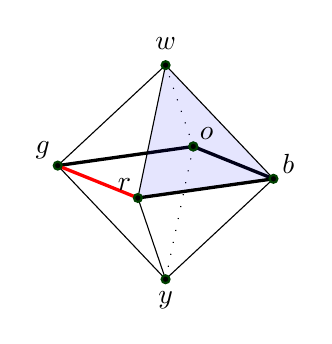
\begin{tikzpicture}%
  [x={(-0.860769cm, -0.121512cm)},
  y={(0.508996cm, -0.205391cm)},
  z={(-0.000053cm, 0.971107cm)},
  scale=1,
  eqback/.style={very thick},
  back/.style={loosely dotted, thin},
  eqedge/.style={very thick},
  edge/.style={black, thin},
  r/.style={red},
  facet/.style={fill=blue!95!black,fill opacity=0.1},
  vertex/.style={inner sep=1pt,circle,draw=green!25!black,fill=black,thick}]
\coordinate (-1, -1, 0) at (-1, -1, 0);
\coordinate (-1, 1, 0) at (-1, 1, 0);
\coordinate (0, 0, -1) at (0, 0, -1);
\coordinate (0, 0, 1) at (0, 0, 1);
\coordinate (1, -1, 0) at (1, -1, 0);
\coordinate (1, 1, 0) at (1, 1, 0);
%% Drawing edges in the back
%%
\draw[edge,eqback] (-1, -1, 0) -- (-1, 1, 0);
\draw[edge,back] (-1, -1, 0) -- (0, 0, -1.4);
\draw[edge,back] (-1, -1, 0) -- (0, 0, 1.4);
\draw[edge,eqback] (1, -1, 0) -- (-1, -1, 0);
%% Drawing vertices in the back
%%
\node[vertex] at (-1, -1, 0)     {};
%% Drawing the facets
%%
%\fill[facet] (1, 1, 0) -- (0, 0, -1.4) -- (1, -1, 0) -- cycle {};
%\fill[facet] (1, 1, 0) -- (0, 0, 1.4) -- (1, -1, 0) -- cycle {};
\fill[facet] (1, 1, 0) -- (-1, 1, 0) -- (0, 0, 1.4) -- cycle {};
%\fill[facet] (1, 1, 0) -- (-1, 1, 0) -- (0, 0, -1.4) -- cycle {};
%% Drawing edges in the front
%%
\draw[edge] (-1, 1, 0) -- (0, 0, -1.4);
\draw[edge] (-1, 1, 0) -- (0, 0, 1.4);
\draw[eqedge] (-1, 1, 0) -- (1, 1, 0);
\draw[edge] (0, 0, -1.4) -- (1, -1, 0);
\draw[edge] (0, 0, -1.4) -- (1, 1, 0);
\draw[edge] (0, 0, 1.4) -- (1, -1, 0);
\draw[edge] (0, 0, 1.4) -- (1, 1, 0);
\draw[r,eqedge] (1, 1, 0) -- (1, -1, 0);
%% Drawing the vertices in the front
%%
\begin{scope}[nodes=vertex]
\node[label=above right:\( b \)] at (-1, 1, 0)     {};
\node[label=below:\( y \)] at (0, 0, -1.4)     {};
\node[label=above:\( w \)] at (0, 0, 1.4)     {};
\node[label=above left:\( g \)] at (1, -1, 0)     {};
\node[label=above left:\( r \)] at (1, 1, 0)     {};
\node[label=above right:\( o \)] at (-1, -1, 0)     {};
\end{scope}
\end{tikzpicture}
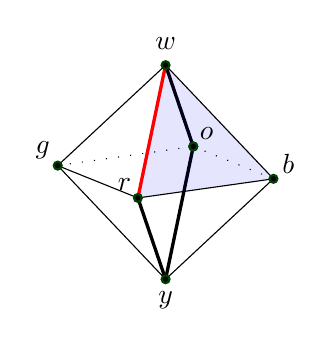
\begin{tikzpicture}%
  [x={(-0.860769cm, -0.121512cm)},
  y={(0.508996cm, -0.205391cm)},
  z={(-0.000053cm, 0.971107cm)},
  scale=1,
  eqback/.style={very thick},
  back/.style={loosely dotted, thin},
  eqedge/.style={very thick},
  r/.style={red},
  edge/.style={black, thin},
  facet/.style={fill=blue!95!black,fill opacity=0.1},
  vertex/.style={inner sep=1pt,circle,draw=green!25!black,fill=black,thick}]
\coordinate (-1, -1, 0) at (-1, -1, 0);
\coordinate (-1, 1, 0) at (-1, 1, 0);
\coordinate (0, 0, -1) at (0, 0, -1);
\coordinate (0, 0, 1) at (0, 0, 1);
\coordinate (1, -1, 0) at (1, -1, 0);
\coordinate (1, 1, 0) at (1, 1, 0);
%% Drawing edges in the back
%%
\draw[edge,back] (-1, -1, 0) -- (-1, 1, 0);
\draw[edge,eqback] (-1, -1, 0) -- (0, 0, -1.4);
\draw[edge,eqback] (0, 0, 1.4) -- (-1, -1, 0);
\draw[edge,back] (1, -1, 0) -- (-1, -1, 0);
%% Drawing vertices in the back
%%
\node[vertex] at (-1, -1, 0)     {};
%% Drawing the facets
%%
% \fill[facet] (1, 1, 0) -- (0, 0, -1.4) -- (1, -1, 0) -- cycle {};
% \fill[facet] (1, 1, 0) -- (0, 0, 1.4) -- (1, -1, 0) -- cycle {};
\fill[facet] (1, 1, 0) -- (-1, 1, 0) -- (0, 0, 1.4) -- cycle {};
% \fill[facet] (1, 1, 0) -- (-1, 1, 0) -- (0, 0, -1.4) -- cycle {};
%% Drawing edges in the front
%%
\draw[edge] (-1, 1, 0) -- (0, 0, -1.4);
\draw[edge] (-1, 1, 0) -- (0, 0, 1.4);
\draw[edge] (-1, 1, 0) -- (1, 1, 0);
\draw[edge] (0, 0, -1.4) -- (1, -1, 0);
\draw[eqedge] (0, 0, -1.4) -- (1, 1, 0);
\draw[edge] (0, 0, 1.4) -- (1, -1, 0);
\draw[r,eqedge] (1, 1, 0) -- (0, 0, 1.4) ;
\draw[edge] (1, 1, 0) -- (1, -1, 0);
%% Drawing the vertices in the front
%%
\begin{scope}[nodes=vertex]
\node[label=above right:\( b \)] at (-1, 1, 0)     {};
\node[label=below:\( y \)] at (0, 0, -1.4)     {};
\node[label=above:\( w \)] at (0, 0, 1.4)     {};
\node[label=above left:\( g \)] at (1, -1, 0)     {};
\node[label=above left:\( r \)] at (1, 1, 0)     {};
\node[label=above right:\( o \)] at (-1, -1, 0)     {};
\end{scope}
\end{tikzpicture}
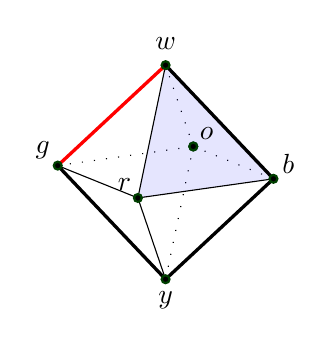
\begin{tikzpicture}%
  [x={(-0.860769cm, -0.121512cm)},
  y={(0.508996cm, -0.205391cm)},
  z={(-0.000053cm, 0.971107cm)},
  scale=1,
  eqback/.style={very thick},
  back/.style={loosely dotted, thin},
  eqedge/.style={very thick},
  r/.style={red},
  edge/.style={black, thin},
  facet/.style={fill=blue!95!black,fill opacity=0.1},
  vertex/.style={inner sep=1pt,circle,draw=green!25!black,fill=black,thick}]
\coordinate (-1, -1, 0) at (-1, -1, 0);
\coordinate (-1, 1, 0) at (-1, 1, 0);
\coordinate (0, 0, -1) at (0, 0, -1);
\coordinate (0, 0, 1) at (0, 0, 1);
\coordinate (1, -1, 0) at (1, -1, 0);
\coordinate (1, 1, 0) at (1, 1, 0);
%% Drawing edges in the back
%%
\draw[edge,back] (-1, -1, 0) -- (-1, 1, 0);
\draw[edge,back] (-1, -1, 0) -- (0, 0, -1.4);
\draw[edge,back] (-1, -1, 0) -- (0, 0, 1.4);
\draw[edge,back] (1, -1, 0) -- (-1, -1, 0);
%% Drawing vertices in the back
%%
\node[vertex] at (-1, -1, 0)     {};
%% Drawing the facets
%%
% \fill[facet] (1, 1, 0) -- (0, 0, -1.4) -- (1, -1, 0) -- cycle {};
% \fill[facet] (1, 1, 0) -- (0, 0, 1.4) -- (1, -1, 0) -- cycle {};
\fill[facet] (1, 1, 0) -- (-1, 1, 0) -- (0, 0, 1.4) -- cycle {};
% \fill[facet] (1, 1, 0) -- (-1, 1, 0) -- (0, 0, -1.4) -- cycle {};
%% Drawing edges in the front
%%
\draw[eqedge] (-1, 1, 0) -- (0, 0, -1.4);
\draw[eqedge] (0, 0, 1.4) -- (-1, 1, 0);
\draw[edge] (-1, 1, 0) -- (1, 1, 0);
\draw[eqedge] (0, 0, -1.4) -- (1, -1, 0);
\draw[edge] (0, 0, -1.4) -- (1, 1, 0);
\draw[r,eqedge] (1, -1, 0) -- (0, 0, 1.4);
\draw[edge] (0, 0, 1.4) -- (1, 1, 0);
\draw[edge] (1, 1, 0) -- (1, -1, 0);
%% Drawing the vertices in the front
%%
\begin{scope}[nodes=vertex]
\node[label=above right:\( b \)] at (-1, 1, 0)     {};
\node[label=below:\( y \)] at (0, 0, -1.4)     {};
\node[label=above:\( w \)] at (0, 0, 1.4)     {};
\node[label=above left:\( g \)] at (1, -1, 0)     {};
\node[label=above left:\( r \)] at (1, 1, 0)     {};
\node[label=above right:\( o \)] at (-1, -1, 0)     {};
\end{scope}
\end{tikzpicture}
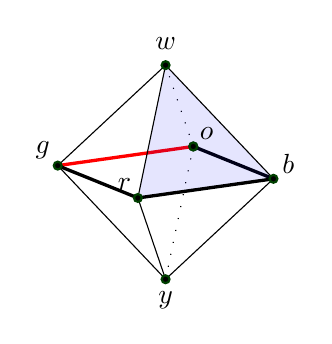
\begin{tikzpicture}%
  [x={(-0.860769cm, -0.121512cm)},
  y={(0.508996cm, -0.205391cm)},
  z={(-0.000053cm, 0.971107cm)},
  scale=1,
  eqback/.style={very thick},
  back/.style={loosely dotted, thin},
  eqedge/.style={very thick},
  edge/.style={black, thin},
  r/.style={red},
  facet/.style={fill=blue!95!black,fill opacity=0.1},
  vertex/.style={inner sep=1pt,circle,draw=green!25!black,fill=black,thick}]
\coordinate (-1, -1, 0) at (-1, -1, 0);
\coordinate (-1, 1, 0) at (-1, 1, 0);
\coordinate (0, 0, -1) at (0, 0, -1);
\coordinate (0, 0, 1) at (0, 0, 1);
\coordinate (1, -1, 0) at (1, -1, 0);
\coordinate (1, 1, 0) at (1, 1, 0);
%% Drawing edges in the back
%%
\draw[edge,eqback] (-1, -1, 0) -- (-1, 1, 0);
\draw[edge,back] (-1, -1, 0) -- (0, 0, -1.4);
\draw[edge,back] (-1, -1, 0) -- (0, 0, 1.4);
\draw[edge,eqback,r] (1, -1, 0) -- (-1, -1, 0);
%% Drawing vertices in the back
%%
\node[vertex] at (-1, -1, 0)     {};
%% Drawing the facets
%%
% \fill[facet] (1, 1, 0) -- (0, 0, -1.4) -- (1, -1, 0) -- cycle {};
% \fill[facet] (1, 1, 0) -- (0, 0, 1.4) -- (1, -1, 0) -- cycle {};
\fill[facet] (1, 1, 0) -- (-1, 1, 0) -- (0, 0, 1.4) -- cycle {};
% \fill[facet] (1, 1, 0) -- (-1, 1, 0) -- (0, 0, -1.4) -- cycle {};
%% Drawing edges in the front
%%
\draw[edge] (-1, 1, 0) -- (0, 0, -1.4);
\draw[edge] (-1, 1, 0) -- (0, 0, 1.4);
\draw[eqedge] (-1, 1, 0) -- (1, 1, 0);
\draw[edge] (0, 0, -1.4) -- (1, -1, 0);
\draw[edge] (0, 0, -1.4) -- (1, 1, 0);
\draw[edge] (0, 0, 1.4) -- (1, -1, 0);
\draw[edge] (0, 0, 1.4) -- (1, 1, 0);
\draw[eqedge] (1, 1, 0) -- (1, -1, 0);
%% Drawing the vertices in the front
%%
\begin{scope}[nodes=vertex]
\node[label=above right:\( b \)] at (-1, 1, 0)     {};
\node[label=below:\( y \)] at (0, 0, -1.4)     {};
\node[label=above:\( w \)] at (0, 0, 1.4)     {};
\node[label=above left:\( g \)] at (1, -1, 0)     {};
\node[label=above left:\( r \)] at (1, 1, 0)     {};
\node[label=above right:\( o \)] at (-1, -1, 0)     {};
\end{scope}
\end{tikzpicture}

\caption{\( \link \) for the vertices \( w, b\) and \( r \).}
\label{fig:triangle_of_equators}
\end{figure}

To extend \( T_0 \) to a function \( T_1 \) on the 1-skeleton we have complete freedom. Defining a map by induction makes clear that the action on paths is its own structure. Two functions on the octahedron could agree on points but differ on edges. We are going to identify this 1-dimensional freedom with a connection:

\begin{mydef}
\label{def:connection}
A \defemph{connection} on a higher combinatorial manifold is an extension of a circle bundle from the 0-skeleton to the 1-skeleton.
\end{mydef}

Continuing the example, we will do something ``tangent bundley'', imagining how \( T_1 \) changes as we slide from point to point in the embedding shown in the figures. Sliding from \( w \) to \( b \) and tipping the link as we go, we see \( r\mapsto r \) and \( o\mapsto o \) because those lie on the axis of rotation. Then \( g\mapsto w \) and \( b\mapsto y \). 

\begin{mydef}
Define \( T_1:\oo_1\to\EMzo \) on just the 1-skeleton by extending \( T_0 \) as follows:
Transport away from \( w \):
\begin{itemize}
\item \( T_1(wb):[b, r, g, o]\mapsto [y, r, w, o] \) (\( r, o \) fixed)
\item \( T_1(wr):[b, r, g, o]\mapsto [b, y, g, w] \) (\( b, g \) fixed)
\item \( T_1(wg):[b, r, g, o]\mapsto [w, r, y, o] \)
\item \( T_1(wo):[b, r, g, o]\mapsto [b, w, g, y] \)
\end{itemize}
Transport away from \( y \):
\begin{itemize}
\item \( T_1(yb):[b, o, g, r]\mapsto [w, o, y, r] \)
\item \( T_1(yr):[b, o, g, r]\mapsto [b, y, g, w] \)
\item \( T_1(yg):[b, o, g, r]\mapsto [y, o, w, r] \)
\item \( T_1(yo):[b, o, g, r]\mapsto [b, w, g, y] \)
\end{itemize}
Transport along the equator:
\begin{itemize}
\item \( T_1(br):[w, o, y, r]\mapsto [w, b, y, g] \) 
\item \( T_1(rg):[w, b, y, g]\mapsto [w, r, y, o] \)
\item \( T_1(go):[w, r, y, o]\mapsto [w, g, y, b] \)
\item \( T_1(ob):[w, g, y, b]\mapsto [w, o, y, r] \)
\end{itemize}
\end{mydef}

It's very important to be able to visualize what \( T_1 \) does to triangular paths such as \( wb\cdot br\cdot rw \) (which circulates around the boundary of face \( wbr \)). You can see it if you imagine Figure~\ref{fig:triangle_of_equators} as the frames of a short movie. Or you can place your palm over the top of a cube and note where your fingers are pointing, then slide your hand to an equatorial face, then along the equator, then back to the top. The answer is: you come back rotated clockwise by a quarter-turn. 

\begin{mydef}
The map \( R:C_4\to C_4 \) rotates by one quarter turn, one ``click":
\begin{multicols}{2}
\begin{itemize}
\item \( R(c_1) = c_2 \)
\item \( R(c_2) = c_3 \)
\item \( R(c_3) = c_4 \)
\item \( R(c_4) = c_1 \)
\item \( R(c_1c_2) = c_2c_3 \)
\item \( R(c_2c_3) = c_3c_4 \)
\item \( R(c_3c_4) = c_4c_1 \)
\item \( R(c_4c_1) = c_1c_2 \)
\end{itemize}
\end{multicols}
\end{mydef}

Note by univalence the equivalence \( R \) gives a loop in the universe, a term of \( C_4=_{\EMzo}C_4 \).

Now let's extend \( T_1 \) to all of \( \oo \) by providing values for the eight faces. The face \( wbr \) is a path from \( \refl_w \) to the concatenation \( wb\cdot br\cdot rw \), and so the image of \( wbr \) under the extended version of \( T_1 \) must be a homotopy from \( \refl_{T_1(w)} \) to \( T_1(wb\cdot br\cdot rw) \). Here \emph{there is no additional freedom}.

\begin{mydef}
Define \( T_2:\oo\to\EMzo \) by extending \( T_1 \) to the faces as follows:
\begin{multicols}{2}
\begin{itemize}
\item \( T_2(wbr)=H_R \) 
\item \( T_2(wrg)=H_R \)
\item \( T_2(wgo)=H_R \)
\item \( T_2(ybo)=H_R \)
\item \( T_2(yrb)=H_R \) 
\item \( T_2(ygr)=H_R \)
\item \( T_2(yog)=H_R \)
\item \( T_2(ybo)=H_R \)
\end{itemize}
\end{multicols}
where \( H_R:R=\refl_{C_4} \) is the obvious homotopy given by composition with \( R^{-1} \). Passing through univalence we get a 2-path between \( R \) and \( \refl \) in the loop space \( C_4=_{\EMzo}C_4 \).
\end{mydef}

\begin{mydef}
\label{def:curvature}
The \defemph{curvature of a connection} on a family \( T:\mm\to\uni \) at a vertex \( v \) of a 2-face \( f \) with boundary path \( p_f \) of a marked presented type \( \mm \) is the automorphism \( \tr(p_f)(Tv) \) together with a homotopy to \( \id_{Tv} \). Since curvature is a proof that the holonomy is the identity, we may also call it a \defemph{flatness structure}.
\end{mydef}

\begin{mynote}
We have defined a function on a cell by requiring it to correspond to the value on the boundary of that cell. This is familiar in classical differential topology, where it's called \emph{the exterior derivative}. The duality of \( d \) and \( \partial \) is recognizable in \( T_2 \), and we might say ``curvature is the derivative of the connection.''
\end{mynote}

\subsection{\texorpdfstring{\( T \)}{T} on concatenations of faces}

A marked presented type has a structure rich enough to perform 1-groupoid and 2-groupoid operations. Consider a subcomplex \( P\subset M \) and use it as a \emph{probe} by composing with the marking maps into \( \mm \):

\begin{center}
% https://q.uiver.app/#q=WzAsOSxbMSwwLCJNXzAiXSxbMSwxLCJNXzEiXSxbMSwyLCJNXzIiXSxbMiwwLCJcXG1hdGhiYntNfV8wIl0sWzIsMSwiXFxtYXRoYmJ7TX1fMSJdLFsyLDIsIlxcbWF0aGJie019XzIiXSxbMCwwLCJQXzAiXSxbMCwxLCJQXzEiXSxbMCwyLCJQXzIiXSxbMCwzLCIqX3YiXSxbMSw0LCIqX2UiXSxbMiw1LCIqX2YiXSxbMCwxLCJpXzEiLDJdLFsxLDIsImlfMiIsMl0sWzMsNCwiXFxtYXRocm17c2t9XzEiXSxbNCw1LCJcXG1hdGhybXtza31fMiJdLFs2LDAsIiIsMCx7InN0eWxlIjp7InRhaWwiOnsibmFtZSI6Imhvb2siLCJzaWRlIjoidG9wIn19fV0sWzcsMSwiIiwwLHsic3R5bGUiOnsidGFpbCI6eyJuYW1lIjoiaG9vayIsInNpZGUiOiJ0b3AifX19XSxbOCwyLCIiLDAseyJzdHlsZSI6eyJ0YWlsIjp7Im5hbWUiOiJob29rIiwic2lkZSI6InRvcCJ9fX1dLFs2LDcsImlfMSIsMl0sWzcsOCwiaV8yIiwyXV0=
\begin{tikzcd}
  {P_0} & {M_0} & {\mathbb{M}_0} \\
  {P_1} & {M_1} & {\mathbb{M}_1} \\
  {P_2} & {M_2} & {\mathbb{M}_2}
  \arrow[hook, from=1-1, to=1-2]
  \arrow["{i_1}"', from=1-1, to=2-1]
  \arrow["{*_v}", from=1-2, to=1-3]
  \arrow["{i_1}"', from=1-2, to=2-2]
  \arrow["{\mathrm{sk}_1}", from=1-3, to=2-3]
  \arrow[hook, from=2-1, to=2-2]
  \arrow["{i_2}"', from=2-1, to=3-1]
  \arrow["{*_e}", from=2-2, to=2-3]
  \arrow["{i_2}"', from=2-2, to=3-2]
  \arrow["{\mathrm{sk}_2}", from=2-3, to=3-3]
  \arrow[hook, from=3-1, to=3-2]
  \arrow["{*_f}", from=3-2, to=3-3]
\end{tikzcd}
\end{center}

For example consider Figure~\ref{fig:concat} and the diamond on the left, which is the image in \( \mm \) of a probe. Denote the clockwise triangular path around the left triangle by \( bcab \), and around the right by \( bdcb \). These are loops at \( b \). Say that the tangent map \( T \) satisfies \( T(bcab)=R \) where \( R \) is some rotation of the 4-sided polygon \( Tb \), and similarly \( T(bdcb)=R \) as well. 

\begin{figure}[htbp]
\centering
\includegraphics[width=250pt]{concat.pdf}
\caption{Concatenating the triangular probes \( bac \) and \( bdc \) in \( \mm \) gives the 4-gon \( abdc \).}
\label{fig:concat}
\end{figure}

Since \( bcab \) has a filler 2-cell, which we will call \( f_1 \), we know that \( T(f_1)=H_R \) where \( H_R:R=\refl \) is a path in \( \Aut(Tb) \) from \( R \) to the identity. Similarly if \( f_2 \) is the filler for \( bdcb \) then \( T(f_2)=H_R \).

The two faces can be horizontally composed giving \( f_1\star f_2 \), which fills the diamond \( bdcab \). Then we also obtain \( T(f_1\star f_2):R^2=\id \).

In this way, given an explicit ordering of the faces (a ``plan'' for visiting all faces of the manifold), we can ``sum'' the curvature. For our ocatahedron where each triangle produces a rotation of \( R \), we'd get \( R^8 \).

\begin{comment}
\subsection{The torus}

We can define a combinatorial torus as a similar HIT. This time each vertex will have six neighbors. So all the links will be merely equal to \( C_6 \) which is a hexagonal version of \( C_4 \). See Figure~\ref{fig:torus}. 

To help parse this figure, imagine instead Figure~\ref{fig:flattorus}. We take this simple alternating-triangle pattern, then glue the left and right edges, then bend into Figure~\ref{fig:torus}. The fact that each column in Figure~\ref{fig:flattorus} has four dots corresponds to the torus in Figure~\ref{fig:torus} having a square in front, diamonds in the middle, and a square in back.

\begin{figure}[htbp]
\centering
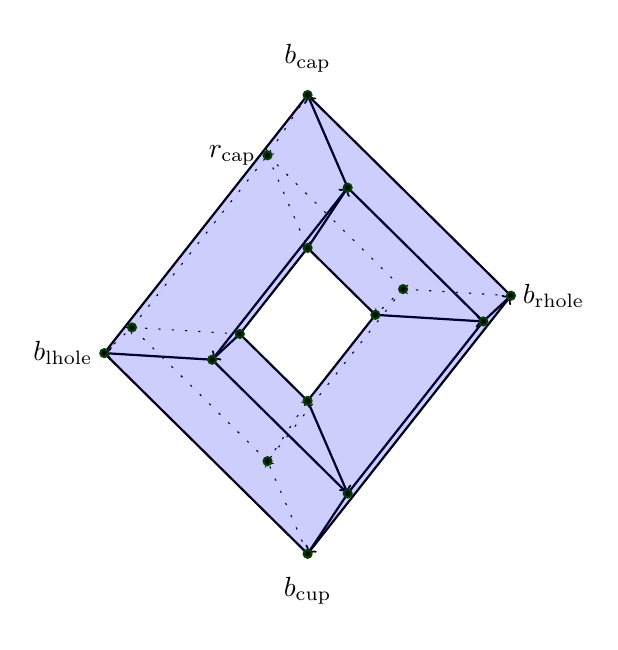
\begin{tikzpicture}%
  [x={(-0.860769cm, -0.121512cm)},
  y={(0.508996cm, -0.205391cm)},
  z={(-0.000053cm, 0.971107cm)},
  scale=1,
  back/.style={loosely dotted, thin},
  edge/.style={->,black, thick},
  line/.style={black, thick},
  facet/.style={fill=blue!95!black,fill opacity=0.1},
  vertex/.style={inner sep=1pt,circle,draw=green!25!black,fill=black,thick}]
\coordinate (r_cap) at (0, -1, 5);
\coordinate (g_cap) at (0, 0, 4 );
\coordinate (o_cap) at (0, 1, 5 );
\coordinate (b_cap) at (0, 0, 6 );

\coordinate (r_cup) at (0, -1, 1);
\coordinate (g_cup) at (0, 0, 2 );
\coordinate (o_cup) at (0, 1, 1 );
\coordinate (b_cup) at (0, 0, 0 );

\coordinate (r_ohole) at (-2, -1, 3);
\coordinate (g_ohole) at (-1, 0,  3);
\coordinate (o_ohole) at (-2, 1,  3);
\coordinate (b_ohole) at (-3, 0,  3);

\coordinate (r_rhole) at (2, -1, 3);
\coordinate (g_rhole) at (1, 0,  3);
\coordinate (o_rhole) at (2, 1,  3);
\coordinate (b_rhole) at (3, 0,  3);

\draw[edge,back] (r_cap) -- (g_cap);
\draw[edge]      (g_cap) -- (o_cap);
\draw[edge]      (o_cap) -- (b_cap);
\draw[edge,back] (b_cap) -- (r_cap);

\draw[edge,back] (r_cup) -- (g_cup);
\draw[edge]      (g_cup) -- (o_cup);
\draw[edge]      (o_cup) -- (b_cup);
\draw[edge,back] (b_cup) -- (r_cup);

\draw[edge,back] (r_ohole) -- (g_ohole);
\draw[edge]      (g_ohole) -- (o_ohole);
\draw[edge]      (o_ohole) -- (b_ohole);
\draw[edge,back] (b_ohole) -- (r_ohole);

\draw[edge,back] (r_rhole) -- (g_rhole);
\draw[edge]      (g_rhole) -- (o_rhole);
\draw[edge]      (o_rhole) -- (b_rhole);
\draw[edge,back] (b_rhole) -- (r_rhole);

\draw[line,back] (r_cap) --   (r_ohole);
\draw[line,back] (r_ohole) -- (r_cup);
\draw[line,back] (r_cup) --   (r_rhole);
\draw[line,back] (r_rhole) -- (r_cap);

\draw[line] (g_cap) --   (g_ohole);
\draw[line] (g_ohole) -- (g_cup);
\draw[line] (g_cup) --   (g_rhole);
\draw[line] (g_rhole) -- (g_cap);

\draw[line] (o_cap) --   (o_ohole);
\draw[line] (o_ohole) -- (o_cup);
\draw[line] (o_cup) --   (o_rhole);
\draw[line] (o_rhole) -- (o_cap);

\draw[line] (b_cap) --   (b_ohole);
\draw[line] (b_ohole) -- (b_cup);
\draw[line] (b_cup) --   (b_rhole);
\draw[line] (b_rhole) -- (b_cap);

\fill[facet] (r_cap) -- (r_ohole) -- (g_ohole) -- (g_cap) -- cycle {};
\fill[facet] (r_cap) -- (r_rhole) -- (g_rhole) -- (g_cap) -- cycle {};
\fill[facet] (r_cap) -- (r_ohole) -- (b_ohole) -- (b_cap) -- cycle {};
\fill[facet] (r_cap) -- (r_rhole) -- (b_rhole) -- (b_cap) -- cycle {};

\fill[facet] (o_cap) -- (o_ohole) -- (g_ohole) -- (g_cap) -- cycle {};
\fill[facet] (o_cap) -- (o_rhole) -- (g_rhole) -- (g_cap) -- cycle {};
\fill[facet] (o_cap) -- (o_ohole) -- (b_ohole) -- (b_cap) -- cycle {};
\fill[facet] (o_cap) -- (o_rhole) -- (b_rhole) -- (b_cap) -- cycle {};

\fill[facet] (r_cup) -- (r_ohole) -- (g_ohole) -- (g_cup) -- cycle {};
\fill[facet] (r_cup) -- (r_rhole) -- (g_rhole) -- (g_cup) -- cycle {};
\fill[facet] (r_cup) -- (r_ohole) -- (b_ohole) -- (b_cup) -- cycle {};
\fill[facet] (r_cup) -- (r_rhole) -- (b_rhole) -- (b_cup) -- cycle {};

\fill[facet] (o_cup) -- (o_ohole) -- (g_ohole) -- (g_cup) -- cycle {};
\fill[facet] (o_cup) -- (o_rhole) -- (g_rhole) -- (g_cup) -- cycle {};
\fill[facet] (o_cup) -- (o_ohole) -- (b_ohole) -- (b_cup) -- cycle {};
\fill[facet] (o_cup) -- (o_rhole) -- (b_rhole) -- (b_cup) -- cycle {};

\begin{scope}[nodes=vertex]
\node[label=left:\( r_{\mathrm{cap}} \)] at (r_cap) {};
\node at (g_cap) {};
\node at (o_cap) {};
\node[label=above:\( b_{\mathrm{cap}} \)] at (b_cap) {};
\node at (r_cup) {};
\node at (g_cup) {};
\node at (o_cup) {};
\node[label=below:\( b_{\mathrm{cup}} \)] at (b_cup) {};
\node at (r_ohole) {};
\node at (g_ohole) {};
\node at (o_ohole) {};
\node[label=right:\( b_{\mathrm{rhole}} \)] at (b_ohole) {};
\node at (r_rhole) {};
\node at (g_rhole) {};
\node at (o_rhole) {};
\node[label=left:\( b_{\mathrm{lhole}} \)] at (b_rhole) {};
\end{scope}
\end{tikzpicture}

\caption{Torus embedded in 3-dimensional space. If you see color in your rendering then black lines trace four square-shaped paths, red ones connect the front square to the middle diamonds, and blue ones connect the back path to the middle ones.}
\label{fig:torus}
\end{figure}

\begin{figure}[htbp]
\centering
% https://q.uiver.app/#q=WzAsMzYsWzEsNCwiXFxidWxsZXQiXSxbMSw2LCJcXGJ1bGxldCJdLFsyLDcsIlxcYnVsbGV0Il0sWzIsNSwiXFxidWxsZXQiXSxbMiwzLCJcXGJ1bGxldCJdLFsxLDgsIlxcYnVsbGV0Il0sWzEsMiwiXFxidWxsZXQiXSxbMywyLCJcXGJ1bGxldCJdLFszLDQsIlxcYnVsbGV0Il0sWzMsNiwiXFxidWxsZXQiXSxbMyw4LCJcXGJ1bGxldCJdLFsyLDEsIlxcYnVsbGV0Il0sWzQsMSwiXFxidWxsZXQiXSxbNSwyLCJcXGJ1bGxldCJdLFs0LDMsIlxcYnVsbGV0Il0sWzUsNCwiXFxidWxsZXQiXSxbNCw1LCJcXGJ1bGxldCJdLFs1LDYsIlxcYnVsbGV0Il0sWzQsNywiXFxidWxsZXQiXSxbNSw4LCJcXGJ1bGxldCJdLFsyLDAsIlxcbWF0aHJte2JhY2t9Il0sWzQsMCwiXFxtYXRocm17ZnJvbnR9Il0sWzEsMCwiXFxtYXRocm17b3V0ZXJ9Il0sWzMsMCwiXFxtYXRocm17aG9sZX0iXSxbNSwwLCJcXG1hdGhybXtvdXRlcn0iXSxbMSwxMCwiXFxidWxsZXQiXSxbMiw5LCJcXGJ1bGxldCJdLFszLDEwLCJcXGJ1bGxldCJdLFs0LDksIlxcYnVsbGV0Il0sWzUsMTAsIlxcYnVsbGV0Il0sWzAsMiwiXFxtYXRocm17dG9wXFwgb2ZcXCBkaWFtb25kc30iXSxbMCw2LCJcXG1hdGhybXtib3R0b21cXCBvZlxcIGRpYW1vbmRzfSJdLFsxLDEsIlxcICJdLFs1LDEsIlxcICJdLFszLDEsIlxcICJdLFswLDEwLCJcXG1hdGhybXt0b3BcXCBvZlxcIGRpYW1vbmRzfSJdLFs0LDMsIiIsMix7InN0eWxlIjp7ImhlYWQiOnsibmFtZSI6Im5vbmUifX19XSxbMywyLCIiLDIseyJzdHlsZSI6eyJoZWFkIjp7Im5hbWUiOiJub25lIn19fV0sWzAsMSwiIiwyLHsic3R5bGUiOnsiaGVhZCI6eyJuYW1lIjoibm9uZSJ9fX1dLFs0LDAsIiIsMSx7ImNvbG91ciI6WzIzNiw5MSw2MF0sInN0eWxlIjp7ImhlYWQiOnsibmFtZSI6Im5vbmUifX19XSxbMCwzLCIiLDEseyJjb2xvdXIiOlsyMzYsOTEsNjBdLCJzdHlsZSI6eyJoZWFkIjp7Im5hbWUiOiJub25lIn19fV0sWzMsMSwiIiwxLHsiY29sb3VyIjpbMjM2LDkxLDYwXSwic3R5bGUiOnsiaGVhZCI6eyJuYW1lIjoibm9uZSJ9fX1dLFsxLDIsIiIsMSx7ImNvbG91ciI6WzIzNiw5MSw2MF0sInN0eWxlIjp7ImhlYWQiOnsibmFtZSI6Im5vbmUifX19XSxbMiw1LCIiLDEseyJjb2xvdXIiOlsyMzYsOTEsNjBdLCJzdHlsZSI6eyJoZWFkIjp7Im5hbWUiOiJub25lIn19fV0sWzEsNSwiIiwxLHsic3R5bGUiOnsiaGVhZCI6eyJuYW1lIjoibm9uZSJ9fX1dLFs2LDQsIiIsMSx7ImNvbG91ciI6WzIzNiw5MSw2MF0sInN0eWxlIjp7ImhlYWQiOnsibmFtZSI6Im5vbmUifX19XSxbNiwwLCIiLDEseyJzdHlsZSI6eyJoZWFkIjp7Im5hbWUiOiJub25lIn19fV0sWzcsOCwiIiwwLHsic3R5bGUiOnsiaGVhZCI6eyJuYW1lIjoibm9uZSJ9fX1dLFs4LDksIiIsMCx7InN0eWxlIjp7ImhlYWQiOnsibmFtZSI6Im5vbmUifX19XSxbOSwxMCwiIiwwLHsic3R5bGUiOnsiaGVhZCI6eyJuYW1lIjoibm9uZSJ9fX1dLFs3LDQsIiIsMCx7ImNvbG91ciI6WzIzNiw5MSw2MF0sInN0eWxlIjp7ImhlYWQiOnsibmFtZSI6Im5vbmUifX19XSxbNCw4LCIiLDAseyJjb2xvdXIiOlsyMzYsOTEsNjBdLCJzdHlsZSI6eyJoZWFkIjp7Im5hbWUiOiJub25lIn19fV0sWzgsMywiIiwwLHsiY29sb3VyIjpbMjM2LDkxLDYwXSwic3R5bGUiOnsiaGVhZCI6eyJuYW1lIjoibm9uZSJ9fX1dLFszLDksIiIsMCx7ImNvbG91ciI6WzIzNiw5MSw2MF0sInN0eWxlIjp7ImhlYWQiOnsibmFtZSI6Im5vbmUifX19XSxbOSwyLCIiLDAseyJjb2xvdXIiOlsyMzYsOTEsNjBdLCJzdHlsZSI6eyJoZWFkIjp7Im5hbWUiOiJub25lIn19fV0sWzIsMTAsIiIsMCx7ImNvbG91ciI6WzIzNiw5MSw2MF0sInN0eWxlIjp7ImhlYWQiOnsibmFtZSI6Im5vbmUifX19XSxbMTEsNCwiIiwwLHsic3R5bGUiOnsiaGVhZCI6eyJuYW1lIjoibm9uZSJ9fX1dLFsxMSw2LCIiLDAseyJjb2xvdXIiOlsyMzYsOTEsNjBdLCJzdHlsZSI6eyJoZWFkIjp7Im5hbWUiOiJub25lIn19fV0sWzExLDcsIiIsMCx7ImNvbG91ciI6WzIzNiw5MSw2MF0sInN0eWxlIjp7ImhlYWQiOnsibmFtZSI6Im5vbmUifX19XSxbMTksMTcsIiIsMCx7InN0eWxlIjp7ImhlYWQiOnsibmFtZSI6Im5vbmUifX19XSxbMTgsMTYsIiIsMCx7InN0eWxlIjp7ImhlYWQiOnsibmFtZSI6Im5vbmUifX19XSxbMTYsMTQsIiIsMCx7InN0eWxlIjp7ImhlYWQiOnsibmFtZSI6Im5vbmUifX19XSxbMTcsMTUsIiIsMCx7InN0eWxlIjp7ImhlYWQiOnsibmFtZSI6Im5vbmUifX19XSxbMTUsMTMsIiIsMCx7InN0eWxlIjp7ImhlYWQiOnsibmFtZSI6Im5vbmUifX19XSxbMTQsMTIsIiIsMCx7InN0eWxlIjp7ImhlYWQiOnsibmFtZSI6Im5vbmUifX19XSxbMTIsNywiIiwwLHsiY29sb3VyIjpbMSw5NSw2MF0sInN0eWxlIjp7ImhlYWQiOnsibmFtZSI6Im5vbmUifX19XSxbMTIsMTMsIiIsMCx7ImNvbG91ciI6WzEsOTUsNjBdLCJzdHlsZSI6eyJoZWFkIjp7Im5hbWUiOiJub25lIn19fV0sWzEzLDE0LCIiLDAseyJjb2xvdXIiOlsxLDk1LDYwXSwic3R5bGUiOnsiaGVhZCI6eyJuYW1lIjoibm9uZSJ9fX1dLFsxNCw4LCIiLDAseyJjb2xvdXIiOlsxLDk1LDYwXSwic3R5bGUiOnsiaGVhZCI6eyJuYW1lIjoibm9uZSJ9fX1dLFsxNCwxNSwiIiwwLHsiY29sb3VyIjpbMSw5NSw2MF0sInN0eWxlIjp7ImhlYWQiOnsibmFtZSI6Im5vbmUifX19XSxbMTUsMTYsIiIsMCx7ImNvbG91ciI6WzEsOTUsNjBdLCJzdHlsZSI6eyJoZWFkIjp7Im5hbWUiOiJub25lIn19fV0sWzgsMTYsIiIsMCx7ImNvbG91ciI6WzEsOTUsNjBdLCJzdHlsZSI6eyJoZWFkIjp7Im5hbWUiOiJub25lIn19fV0sWzE2LDksIiIsMCx7ImNvbG91ciI6WzEsOTUsNjBdLCJzdHlsZSI6eyJoZWFkIjp7Im5hbWUiOiJub25lIn19fV0sWzE2LDE3LCIiLDAseyJjb2xvdXIiOlsxLDk1LDYwXSwic3R5bGUiOnsiaGVhZCI6eyJuYW1lIjoibm9uZSJ9fX1dLFsxNywxOCwiIiwwLHsiY29sb3VyIjpbMSw5NSw2MF0sInN0eWxlIjp7ImhlYWQiOnsibmFtZSI6Im5vbmUifX19XSxbOSwxOCwiIiwwLHsiY29sb3VyIjpbMSw5NSw2MF0sInN0eWxlIjp7ImhlYWQiOnsibmFtZSI6Im5vbmUifX19XSxbMTgsMTksIiIsMCx7ImNvbG91ciI6WzEsOTUsNjBdLCJzdHlsZSI6eyJoZWFkIjp7Im5hbWUiOiJub25lIn19fV0sWzE4LDEwLCIiLDAseyJjb2xvdXIiOlsxLDk1LDYwXSwic3R5bGUiOnsiaGVhZCI6eyJuYW1lIjoibm9uZSJ9fX1dLFs3LDE0LCIiLDAseyJjb2xvdXIiOlsxLDk1LDYwXSwic3R5bGUiOnsiaGVhZCI6eyJuYW1lIjoibm9uZSJ9fX1dLFs1LDI2LCIiLDEseyJjb2xvdXIiOlsyMzYsOTEsNjBdLCJzdHlsZSI6eyJoZWFkIjp7Im5hbWUiOiJub25lIn19fV0sWzEwLDI2LCIiLDEseyJjb2xvdXIiOlsyMzYsOTEsNjBdLCJzdHlsZSI6eyJoZWFkIjp7Im5hbWUiOiJub25lIn19fV0sWzIsMjYsIiIsMSx7InN0eWxlIjp7ImhlYWQiOnsibmFtZSI6Im5vbmUifX19XSxbMTgsMjgsIiIsMSx7InN0eWxlIjp7ImhlYWQiOnsibmFtZSI6Im5vbmUifX19XSxbMjYsMjUsIiIsMSx7ImNvbG91ciI6WzIzNiw5MSw2MF0sInN0eWxlIjp7ImhlYWQiOnsibmFtZSI6Im5vbmUifX19XSxbMjYsMjcsIiIsMSx7ImNvbG91ciI6WzIzNiw5MSw2MF0sInN0eWxlIjp7ImhlYWQiOnsibmFtZSI6Im5vbmUifX19XSxbMjgsMjksIiIsMSx7ImNvbG91ciI6WzEsOTUsNjBdLCJzdHlsZSI6eyJoZWFkIjp7Im5hbWUiOiJub25lIn19fV0sWzE5LDI5LCIiLDEseyJzdHlsZSI6eyJoZWFkIjp7Im5hbWUiOiJub25lIn19fV0sWzEwLDI3LCIiLDEseyJzdHlsZSI6eyJoZWFkIjp7Im5hbWUiOiJub25lIn19fV0sWzUsMjUsIiIsMSx7InN0eWxlIjp7ImhlYWQiOnsibmFtZSI6Im5vbmUifX19XSxbMjgsMjcsIiIsMSx7ImNvbG91ciI6WzEsOTUsNjBdLCJzdHlsZSI6eyJoZWFkIjp7Im5hbWUiOiJub25lIn19fV0sWzI4LDE5LCIiLDEseyJjb2xvdXIiOlsxLDk1LDYwXSwic3R5bGUiOnsiaGVhZCI6eyJuYW1lIjoibm9uZSJ9fX1dLFsyOCwxMCwiIiwxLHsiY29sb3VyIjpbMSw5NSw2MF0sInN0eWxlIjp7ImhlYWQiOnsibmFtZSI6Im5vbmUifX19XSxbMzAsNiwiIiwxLHsic3R5bGUiOnsiYm9keSI6eyJuYW1lIjoiZG90dGVkIn19fV0sWzMxLDEsIiIsMSx7InN0eWxlIjp7ImJvZHkiOnsibmFtZSI6ImRvdHRlZCJ9fX1dLFsyMCwxMSwiIiwwLHsic3R5bGUiOnsiYm9keSI6eyJuYW1lIjoiZG90dGVkIn19fV0sWzIxLDEyLCIiLDAseyJzdHlsZSI6eyJib2R5Ijp7Im5hbWUiOiJkb3R0ZWQifX19XSxbMjIsMzIsIiIsMCx7InN0eWxlIjp7ImJvZHkiOnsibmFtZSI6ImRvdHRlZCJ9fX1dLFsyNCwzMywiIiwwLHsic3R5bGUiOnsiYm9keSI6eyJuYW1lIjoiZG90dGVkIn19fV0sWzIzLDM0LCIiLDAseyJzdHlsZSI6eyJib2R5Ijp7Im5hbWUiOiJkb3R0ZWQifX19XSxbMzUsMjUsIiIsMSx7InN0eWxlIjp7ImJvZHkiOnsibmFtZSI6ImRvdHRlZCJ9fX1dXQ==
\begin{tikzcd}[column sep=1ex,row sep=1ex]
	& {\mathrm{outer}} & {\mathrm{back}} & {\mathrm{hole}} & {\mathrm{front}} & {\mathrm{outer}} \\
	& {\ } & \bullet & {\ } & \bullet & {\ } \\
	{\mathrm{top\ of\ diamonds}} & \bullet && \bullet && \bullet \\
	&& \bullet && \bullet \\
	& \bullet && \bullet && \bullet \\
	&& \bullet && \bullet \\
	{\mathrm{bottom\ of\ diamonds}} & \bullet && \bullet && \bullet \\
	&& \bullet && \bullet \\
	& \bullet && \bullet && \bullet \\
	&& \bullet && \bullet \\
	{\mathrm{top\ of\ diamonds}} & \bullet && \bullet && \bullet
	\arrow[dotted, from=1-2, to=2-2]
	\arrow[dotted, from=1-3, to=2-3]
	\arrow[dotted, from=1-4, to=2-4]
	\arrow[dotted, from=1-5, to=2-5]
	\arrow[dotted, from=1-6, to=2-6]
	\arrow[draw={rgb,255:red,60;green,73;blue,246}, no head, from=2-3, to=3-2]
	\arrow[draw={rgb,255:red,60;green,73;blue,246}, no head, from=2-3, to=3-4]
	\arrow[no head, from=2-3, to=4-3]
	\arrow[draw={rgb,255:red,250;green,59;blue,56}, no head, from=2-5, to=3-4]
	\arrow[draw={rgb,255:red,250;green,59;blue,56}, no head, from=2-5, to=3-6]
	\arrow[dotted, from=3-1, to=3-2]
	\arrow[draw={rgb,255:red,60;green,73;blue,246}, no head, from=3-2, to=4-3]
	\arrow[no head, from=3-2, to=5-2]
	\arrow[draw={rgb,255:red,60;green,73;blue,246}, no head, from=3-4, to=4-3]
	\arrow[draw={rgb,255:red,250;green,59;blue,56}, no head, from=3-4, to=4-5]
	\arrow[no head, from=3-4, to=5-4]
	\arrow[draw={rgb,255:red,250;green,59;blue,56}, no head, from=3-6, to=4-5]
	\arrow[draw={rgb,255:red,60;green,73;blue,246}, no head, from=4-3, to=5-2]
	\arrow[draw={rgb,255:red,60;green,73;blue,246}, no head, from=4-3, to=5-4]
	\arrow[no head, from=4-3, to=6-3]
	\arrow[no head, from=4-5, to=2-5]
	\arrow[draw={rgb,255:red,250;green,59;blue,56}, no head, from=4-5, to=5-4]
	\arrow[draw={rgb,255:red,250;green,59;blue,56}, no head, from=4-5, to=5-6]
	\arrow[draw={rgb,255:red,60;green,73;blue,246}, no head, from=5-2, to=6-3]
	\arrow[no head, from=5-2, to=7-2]
	\arrow[draw={rgb,255:red,60;green,73;blue,246}, no head, from=5-4, to=6-3]
	\arrow[draw={rgb,255:red,250;green,59;blue,56}, no head, from=5-4, to=6-5]
	\arrow[no head, from=5-4, to=7-4]
	\arrow[no head, from=5-6, to=3-6]
	\arrow[draw={rgb,255:red,250;green,59;blue,56}, no head, from=5-6, to=6-5]
	\arrow[draw={rgb,255:red,60;green,73;blue,246}, no head, from=6-3, to=7-2]
	\arrow[draw={rgb,255:red,60;green,73;blue,246}, no head, from=6-3, to=7-4]
	\arrow[no head, from=6-3, to=8-3]
	\arrow[no head, from=6-5, to=4-5]
	\arrow[draw={rgb,255:red,250;green,59;blue,56}, no head, from=6-5, to=7-4]
	\arrow[draw={rgb,255:red,250;green,59;blue,56}, no head, from=6-5, to=7-6]
	\arrow[dotted, from=7-1, to=7-2]
	\arrow[draw={rgb,255:red,60;green,73;blue,246}, no head, from=7-2, to=8-3]
	\arrow[no head, from=7-2, to=9-2]
	\arrow[draw={rgb,255:red,60;green,73;blue,246}, no head, from=7-4, to=8-3]
	\arrow[draw={rgb,255:red,250;green,59;blue,56}, no head, from=7-4, to=8-5]
	\arrow[no head, from=7-4, to=9-4]
	\arrow[no head, from=7-6, to=5-6]
	\arrow[draw={rgb,255:red,250;green,59;blue,56}, no head, from=7-6, to=8-5]
	\arrow[draw={rgb,255:red,60;green,73;blue,246}, no head, from=8-3, to=9-2]
	\arrow[draw={rgb,255:red,60;green,73;blue,246}, no head, from=8-3, to=9-4]
	\arrow[no head, from=8-3, to=10-3]
	\arrow[no head, from=8-5, to=6-5]
	\arrow[draw={rgb,255:red,250;green,59;blue,56}, no head, from=8-5, to=9-4]
	\arrow[draw={rgb,255:red,250;green,59;blue,56}, no head, from=8-5, to=9-6]
	\arrow[no head, from=8-5, to=10-5]
	\arrow[color={rgb,255:red,60;green,73;blue,246}, no head, from=9-2, to=10-3]
	\arrow[no head, from=9-2, to=11-2]
	\arrow[color={rgb,255:red,60;green,73;blue,246}, no head, from=9-4, to=10-3]
	\arrow[no head, from=9-4, to=11-4]
	\arrow[no head, from=9-6, to=7-6]
	\arrow[no head, from=9-6, to=11-6]
	\arrow[color={rgb,255:red,60;green,73;blue,246}, no head, from=10-3, to=11-2]
	\arrow[color={rgb,255:red,60;green,73;blue,246}, no head, from=10-3, to=11-4]
	\arrow[color={rgb,255:red,250;green,59;blue,56}, no head, from=10-5, to=9-4]
	\arrow[color={rgb,255:red,250;green,59;blue,56}, no head, from=10-5, to=9-6]
	\arrow[color={rgb,255:red,250;green,59;blue,56}, no head, from=10-5, to=11-4]
	\arrow[color={rgb,255:red,250;green,59;blue,56}, no head, from=10-5, to=11-6]
	\arrow[dotted, from=11-1, to=11-2]
\end{tikzcd}

\caption{An inspiration for the torus. Identify the sides and then the top, definitionally, to get the actual torus.}
\label{fig:flattorus}
\end{figure}

This somewhat arbitrary and unfamiliar model of a torus has the helpful property that it is a combinatorial manifold that is somewhat minimal while still being representable by a donut shape. But the donut-shaped version suggests a very different connection than the flat model! Starting with the flat model, we can easily see how to define \( T_1 \) by sliding a link rigidly along the page to the link of some adjacent vertex. Then we can see that transport around any loop is the identity and so \( T_2 \) is always the identity (together with the homotopy \( \refl_\id \) from the identity to itself). So if we imagine a way to visit every face like we did for the octahedron, starting and ending at some basepoint \( v \), we expect to see no net rotation at all of \( Tv \). Later we will call this ``total curvature 0.''

The donut-shaped torus suggests a different connection, one determined by the embedding in 3-space that we have represented. But the easiest way to think about that bundle and its connection and curvature is to wait until we have a proof of the Poincaré-Hopf theorem, so that we can instead compute with a vector field.
\end{comment}

\subsection{Existence of connections}

How confident can we be that we can always define a connection on an arbitrary combinatorial manifold? Two things make the octahedron example special: the link is a 4-gon at every vertex, and every edge extends to a symmetry of the entire octahedron, embedded in 3-dimensional space. This imposed a coherence on the interactions of all the choices we made for the connection, which we can worry may not exist for more complex combinatorial data.

We know as a fact outside of HoTT that any combinatorial surface that has been realized as a triangulated surface embedded in 3-dimensional euclidean space can inherit the parallel transport entailed in the embedding. We could then approximate that data to arbitrary precision with enough subdivision of the fibers of \( T \).

What would a proof inside of HoTT look like? We will leave this as an open question.


%\clearpage
\section{Vector fields}

\begin{mydef}
A \defemph{partial function} \( f:A\to B \) is a function \( f:A\to B+\star \), the disjoint union of \( B \) with the 1-element type.
\end{mydef}

If \( T:\mm\to\EMzo \) is a bundle of mere circles, then a vector field should be a partial function \( T_\bullet:\mm\to\EMpzo \) that lifts \( T \). In other words, a pointing of \emph{some} of the fibers. This aligns with the classical picture of a choice of nonzero vector at each point, except for some points where the vector field vanishes. So instead of having a notion corresponding to the full tangent vector space (one candidate for which would be the disk at each point, i.e. \( \link \) plus its spokes and filler triangles) we are mapping some vertices to their circular fibers, and others to \( \star \). This lets us continue to work with \( \EMzo \) instead of a type of tangent spaces.

Figure~\ref{fig:flattorus_zero} illustrates what removing the preimage of \( \star \) looks like. The resulting type is no longer a combinatorial manifold, since it fails the condition about every point having a circular link. 

\begin{figure}[htbp]
\centering
% https://q.uiver.app/#q=WzAsMzUsWzEsNCwiXFxidWxsZXQiXSxbMSw2LCJcXGJ1bGxldCJdLFsyLDcsIlxcYnVsbGV0Il0sWzIsNSwiXFxidWxsZXQiXSxbMiwzLCJcXGJ1bGxldCJdLFsxLDgsIlxcYnVsbGV0Il0sWzEsMiwiXFxidWxsZXQiXSxbMywyLCJcXGJ1bGxldCJdLFszLDQsIlxcYnVsbGV0Il0sWzMsOCwiXFxidWxsZXQiXSxbMiwxLCJcXGJ1bGxldCJdLFs0LDEsIlxcYnVsbGV0Il0sWzUsMiwiXFxidWxsZXQiXSxbNCwzLCJcXGJ1bGxldCJdLFs1LDQsIlxcYnVsbGV0Il0sWzQsNSwiXFxidWxsZXQiXSxbNSw2LCJcXGJ1bGxldCJdLFs0LDcsIlxcYnVsbGV0Il0sWzUsOCwiXFxidWxsZXQiXSxbMiwwLCJcXG1hdGhybXtiYWNrfSJdLFs0LDAsIlxcbWF0aHJte2Zyb250fSJdLFsxLDAsIlxcbWF0aHJte291dGVyfSJdLFszLDAsIlxcbWF0aHJte2hvbGV9Il0sWzUsMCwiXFxtYXRocm17b3V0ZXJ9Il0sWzEsMTAsIlxcYnVsbGV0Il0sWzIsOSwiXFxidWxsZXQiXSxbMywxMCwiXFxidWxsZXQiXSxbNCw5LCJcXGJ1bGxldCJdLFs1LDEwLCJcXGJ1bGxldCJdLFswLDIsIlxcbWF0aHJte3RvcFxcIG9mXFwgZGlhbW9uZHN9Il0sWzAsNiwiXFxtYXRocm17Ym90dG9tXFwgb2ZcXCBkaWFtb25kc30iXSxbMSwxLCJcXCAiXSxbNSwxLCJcXCAiXSxbMywxLCJcXCAiXSxbMCwxMCwiXFxtYXRocm17dG9wXFwgb2ZcXCBkaWFtb25kc30iXSxbNCwzLCIiLDIseyJzdHlsZSI6eyJoZWFkIjp7Im5hbWUiOiJub25lIn19fV0sWzMsMiwiIiwyLHsic3R5bGUiOnsiaGVhZCI6eyJuYW1lIjoibm9uZSJ9fX1dLFswLDEsIiIsMix7InN0eWxlIjp7ImhlYWQiOnsibmFtZSI6Im5vbmUifX19XSxbNCwwLCIiLDEseyJjb2xvdXIiOlsyMzYsOTEsNjBdLCJzdHlsZSI6eyJoZWFkIjp7Im5hbWUiOiJub25lIn19fV0sWzAsMywiIiwxLHsiY29sb3VyIjpbMjM2LDkxLDYwXSwic3R5bGUiOnsiaGVhZCI6eyJuYW1lIjoibm9uZSJ9fX1dLFszLDEsIiIsMSx7ImNvbG91ciI6WzIzNiw5MSw2MF0sInN0eWxlIjp7ImhlYWQiOnsibmFtZSI6Im5vbmUifX19XSxbMSwyLCIiLDEseyJjb2xvdXIiOlsyMzYsOTEsNjBdLCJzdHlsZSI6eyJoZWFkIjp7Im5hbWUiOiJub25lIn19fV0sWzIsNSwiIiwxLHsiY29sb3VyIjpbMjM2LDkxLDYwXSwic3R5bGUiOnsiaGVhZCI6eyJuYW1lIjoibm9uZSJ9fX1dLFsxLDUsIiIsMSx7InN0eWxlIjp7ImhlYWQiOnsibmFtZSI6Im5vbmUifX19XSxbNiw0LCIiLDEseyJjb2xvdXIiOlsyMzYsOTEsNjBdLCJzdHlsZSI6eyJoZWFkIjp7Im5hbWUiOiJub25lIn19fV0sWzYsMCwiIiwxLHsic3R5bGUiOnsiaGVhZCI6eyJuYW1lIjoibm9uZSJ9fX1dLFs3LDgsIiIsMCx7InN0eWxlIjp7ImhlYWQiOnsibmFtZSI6Im5vbmUifX19XSxbNyw0LCIiLDAseyJjb2xvdXIiOlsyMzYsOTEsNjBdLCJzdHlsZSI6eyJoZWFkIjp7Im5hbWUiOiJub25lIn19fV0sWzQsOCwiIiwwLHsiY29sb3VyIjpbMjM2LDkxLDYwXSwic3R5bGUiOnsiaGVhZCI6eyJuYW1lIjoibm9uZSJ9fX1dLFs4LDMsIiIsMCx7ImNvbG91ciI6WzIzNiw5MSw2MF0sInN0eWxlIjp7ImhlYWQiOnsibmFtZSI6Im5vbmUifX19XSxbMiw5LCIiLDAseyJjb2xvdXIiOlsyMzYsOTEsNjBdLCJzdHlsZSI6eyJoZWFkIjp7Im5hbWUiOiJub25lIn19fV0sWzEwLDQsIiIsMCx7InN0eWxlIjp7ImhlYWQiOnsibmFtZSI6Im5vbmUifX19XSxbMTAsNiwiIiwwLHsiY29sb3VyIjpbMjM2LDkxLDYwXSwic3R5bGUiOnsiaGVhZCI6eyJuYW1lIjoibm9uZSJ9fX1dLFsxMCw3LCIiLDAseyJjb2xvdXIiOlsyMzYsOTEsNjBdLCJzdHlsZSI6eyJoZWFkIjp7Im5hbWUiOiJub25lIn19fV0sWzE4LDE2LCIiLDAseyJzdHlsZSI6eyJoZWFkIjp7Im5hbWUiOiJub25lIn19fV0sWzE3LDE1LCIiLDAseyJzdHlsZSI6eyJoZWFkIjp7Im5hbWUiOiJub25lIn19fV0sWzE1LDEzLCIiLDAseyJzdHlsZSI6eyJoZWFkIjp7Im5hbWUiOiJub25lIn19fV0sWzE2LDE0LCIiLDAseyJzdHlsZSI6eyJoZWFkIjp7Im5hbWUiOiJub25lIn19fV0sWzE0LDEyLCIiLDAseyJzdHlsZSI6eyJoZWFkIjp7Im5hbWUiOiJub25lIn19fV0sWzEzLDExLCIiLDAseyJzdHlsZSI6eyJoZWFkIjp7Im5hbWUiOiJub25lIn19fV0sWzExLDcsIiIsMCx7ImNvbG91ciI6WzEsOTUsNjBdLCJzdHlsZSI6eyJoZWFkIjp7Im5hbWUiOiJub25lIn19fV0sWzExLDEyLCIiLDAseyJjb2xvdXIiOlsxLDk1LDYwXSwic3R5bGUiOnsiaGVhZCI6eyJuYW1lIjoibm9uZSJ9fX1dLFsxMiwxMywiIiwwLHsiY29sb3VyIjpbMSw5NSw2MF0sInN0eWxlIjp7ImhlYWQiOnsibmFtZSI6Im5vbmUifX19XSxbMTMsOCwiIiwwLHsiY29sb3VyIjpbMSw5NSw2MF0sInN0eWxlIjp7ImhlYWQiOnsibmFtZSI6Im5vbmUifX19XSxbMTMsMTQsIiIsMCx7ImNvbG91ciI6WzEsOTUsNjBdLCJzdHlsZSI6eyJoZWFkIjp7Im5hbWUiOiJub25lIn19fV0sWzE0LDE1LCIiLDAseyJjb2xvdXIiOlsxLDk1LDYwXSwic3R5bGUiOnsiaGVhZCI6eyJuYW1lIjoibm9uZSJ9fX1dLFs4LDE1LCIiLDAseyJjb2xvdXIiOlsxLDk1LDYwXSwic3R5bGUiOnsiaGVhZCI6eyJuYW1lIjoibm9uZSJ9fX1dLFsxNSwxNiwiIiwwLHsiY29sb3VyIjpbMSw5NSw2MF0sInN0eWxlIjp7ImhlYWQiOnsibmFtZSI6Im5vbmUifX19XSxbMTYsMTcsIiIsMCx7ImNvbG91ciI6WzEsOTUsNjBdLCJzdHlsZSI6eyJoZWFkIjp7Im5hbWUiOiJub25lIn19fV0sWzE3LDE4LCIiLDAseyJjb2xvdXIiOlsxLDk1LDYwXSwic3R5bGUiOnsiaGVhZCI6eyJuYW1lIjoibm9uZSJ9fX1dLFsxNyw5LCIiLDAseyJjb2xvdXIiOlsxLDk1LDYwXSwic3R5bGUiOnsiaGVhZCI6eyJuYW1lIjoibm9uZSJ9fX1dLFs3LDEzLCIiLDAseyJjb2xvdXIiOlsxLDk1LDYwXSwic3R5bGUiOnsiaGVhZCI6eyJuYW1lIjoibm9uZSJ9fX1dLFs1LDI1LCIiLDEseyJjb2xvdXIiOlsyMzYsOTEsNjBdLCJzdHlsZSI6eyJoZWFkIjp7Im5hbWUiOiJub25lIn19fV0sWzksMjUsIiIsMSx7ImNvbG91ciI6WzIzNiw5MSw2MF0sInN0eWxlIjp7ImhlYWQiOnsibmFtZSI6Im5vbmUifX19XSxbMiwyNSwiIiwxLHsic3R5bGUiOnsiaGVhZCI6eyJuYW1lIjoibm9uZSJ9fX1dLFsxNywyNywiIiwxLHsic3R5bGUiOnsiaGVhZCI6eyJuYW1lIjoibm9uZSJ9fX1dLFsyNSwyNCwiIiwxLHsiY29sb3VyIjpbMjM2LDkxLDYwXSwic3R5bGUiOnsiaGVhZCI6eyJuYW1lIjoibm9uZSJ9fX1dLFsyNSwyNiwiIiwxLHsiY29sb3VyIjpbMjM2LDkxLDYwXSwic3R5bGUiOnsiaGVhZCI6eyJuYW1lIjoibm9uZSJ9fX1dLFsyNywyOCwiIiwxLHsiY29sb3VyIjpbMSw5NSw2MF0sInN0eWxlIjp7ImhlYWQiOnsibmFtZSI6Im5vbmUifX19XSxbMTgsMjgsIiIsMSx7InN0eWxlIjp7ImhlYWQiOnsibmFtZSI6Im5vbmUifX19XSxbOSwyNiwiIiwxLHsic3R5bGUiOnsiaGVhZCI6eyJuYW1lIjoibm9uZSJ9fX1dLFs1LDI0LCIiLDEseyJzdHlsZSI6eyJoZWFkIjp7Im5hbWUiOiJub25lIn19fV0sWzI3LDI2LCIiLDEseyJjb2xvdXIiOlsxLDk1LDYwXSwic3R5bGUiOnsiaGVhZCI6eyJuYW1lIjoibm9uZSJ9fX1dLFsyNywxOCwiIiwxLHsiY29sb3VyIjpbMSw5NSw2MF0sInN0eWxlIjp7ImhlYWQiOnsibmFtZSI6Im5vbmUifX19XSxbMjcsOSwiIiwxLHsiY29sb3VyIjpbMSw5NSw2MF0sInN0eWxlIjp7ImhlYWQiOnsibmFtZSI6Im5vbmUifX19XSxbMjksNiwiIiwxLHsic3R5bGUiOnsiYm9keSI6eyJuYW1lIjoiZG90dGVkIn19fV0sWzMwLDEsIiIsMSx7InN0eWxlIjp7ImJvZHkiOnsibmFtZSI6ImRvdHRlZCJ9fX1dLFsxOSwxMCwiIiwwLHsic3R5bGUiOnsiYm9keSI6eyJuYW1lIjoiZG90dGVkIn19fV0sWzIwLDExLCIiLDAseyJzdHlsZSI6eyJib2R5Ijp7Im5hbWUiOiJkb3R0ZWQifX19XSxbMjEsMzEsIiIsMCx7InN0eWxlIjp7ImJvZHkiOnsibmFtZSI6ImRvdHRlZCJ9fX1dLFsyMywzMiwiIiwwLHsic3R5bGUiOnsiYm9keSI6eyJuYW1lIjoiZG90dGVkIn19fV0sWzIyLDMzLCIiLDAseyJzdHlsZSI6eyJib2R5Ijp7Im5hbWUiOiJkb3R0ZWQifX19XSxbMzQsMjQsIiIsMSx7InN0eWxlIjp7ImJvZHkiOnsibmFtZSI6ImRvdHRlZCJ9fX1dXQ==
\begin{tikzcd}[column sep=1ex,row sep=1ex]
  & {\mathrm{outer}} & {\mathrm{back}} & {\mathrm{hole}} & {\mathrm{front}} & {\mathrm{outer}} \\
  & {\ } & \bullet & {\ } & \bullet & {\ } \\
  {\mathrm{top\ of\ diamonds}} & \bullet && \bullet && \bullet \\
  && \bullet && \bullet \\
  & \bullet && \bullet && \bullet \\
  && \bullet && \bullet \\
  {\mathrm{bottom\ of\ diamonds}} & \bullet &&&& \bullet \\
  && \bullet && \bullet \\
  & \bullet && \bullet && \bullet \\
  && \bullet && \bullet \\
  {\mathrm{top\ of\ diamonds}} & \bullet && \bullet && \bullet
  \arrow[dotted, from=1-2, to=2-2]
  \arrow[dotted, from=1-3, to=2-3]
  \arrow[dotted, from=1-4, to=2-4]
  \arrow[dotted, from=1-5, to=2-5]
  \arrow[dotted, from=1-6, to=2-6]
  \arrow[draw={rgb,255:red,60;green,73;blue,246}, no head, from=2-3, to=3-2]
  \arrow[draw={rgb,255:red,60;green,73;blue,246}, no head, from=2-3, to=3-4]
  \arrow[no head, from=2-3, to=4-3]
  \arrow[draw={rgb,255:red,250;green,59;blue,56}, no head, from=2-5, to=3-4]
  \arrow[draw={rgb,255:red,250;green,59;blue,56}, no head, from=2-5, to=3-6]
  \arrow[dotted, from=3-1, to=3-2]
  \arrow[draw={rgb,255:red,60;green,73;blue,246}, no head, from=3-2, to=4-3]
  \arrow[no head, from=3-2, to=5-2]
  \arrow[draw={rgb,255:red,60;green,73;blue,246}, no head, from=3-4, to=4-3]
  \arrow[draw={rgb,255:red,250;green,59;blue,56}, no head, from=3-4, to=4-5]
  \arrow[no head, from=3-4, to=5-4]
  \arrow[draw={rgb,255:red,250;green,59;blue,56}, no head, from=3-6, to=4-5]
  \arrow[draw={rgb,255:red,60;green,73;blue,246}, no head, from=4-3, to=5-2]
  \arrow[draw={rgb,255:red,60;green,73;blue,246}, no head, from=4-3, to=5-4]
  \arrow[no head, from=4-3, to=6-3]
  \arrow[no head, from=4-5, to=2-5]
  \arrow[draw={rgb,255:red,250;green,59;blue,56}, no head, from=4-5, to=5-4]
  \arrow[draw={rgb,255:red,250;green,59;blue,56}, no head, from=4-5, to=5-6]
  \arrow[draw={rgb,255:red,60;green,73;blue,246}, no head, from=5-2, to=6-3]
  \arrow[no head, from=5-2, to=7-2]
  \arrow[draw={rgb,255:red,60;green,73;blue,246}, no head, from=5-4, to=6-3]
  \arrow[draw={rgb,255:red,250;green,59;blue,56}, no head, from=5-4, to=6-5]
  \arrow[no head, from=5-6, to=3-6]
  \arrow[draw={rgb,255:red,250;green,59;blue,56}, no head, from=5-6, to=6-5]
  \arrow[draw={rgb,255:red,60;green,73;blue,246}, no head, from=6-3, to=7-2]
  \arrow[no head, from=6-3, to=8-3]
  \arrow[no head, from=6-5, to=4-5]
  \arrow[draw={rgb,255:red,250;green,59;blue,56}, no head, from=6-5, to=7-6]
  \arrow[dotted, from=7-1, to=7-2]
  \arrow[draw={rgb,255:red,60;green,73;blue,246}, no head, from=7-2, to=8-3]
  \arrow[no head, from=7-2, to=9-2]
  \arrow[no head, from=7-6, to=5-6]
  \arrow[draw={rgb,255:red,250;green,59;blue,56}, no head, from=7-6, to=8-5]
  \arrow[draw={rgb,255:red,60;green,73;blue,246}, no head, from=8-3, to=9-2]
  \arrow[draw={rgb,255:red,60;green,73;blue,246}, no head, from=8-3, to=9-4]
  \arrow[no head, from=8-3, to=10-3]
  \arrow[no head, from=8-5, to=6-5]
  \arrow[draw={rgb,255:red,250;green,59;blue,56}, no head, from=8-5, to=9-4]
  \arrow[draw={rgb,255:red,250;green,59;blue,56}, no head, from=8-5, to=9-6]
  \arrow[no head, from=8-5, to=10-5]
  \arrow[draw={rgb,255:red,60;green,73;blue,246}, no head, from=9-2, to=10-3]
  \arrow[no head, from=9-2, to=11-2]
  \arrow[draw={rgb,255:red,60;green,73;blue,246}, no head, from=9-4, to=10-3]
  \arrow[no head, from=9-4, to=11-4]
  \arrow[no head, from=9-6, to=7-6]
  \arrow[no head, from=9-6, to=11-6]
  \arrow[draw={rgb,255:red,60;green,73;blue,246}, no head, from=10-3, to=11-2]
  \arrow[draw={rgb,255:red,60;green,73;blue,246}, no head, from=10-3, to=11-4]
  \arrow[draw={rgb,255:red,250;green,59;blue,56}, no head, from=10-5, to=9-4]
  \arrow[draw={rgb,255:red,250;green,59;blue,56}, no head, from=10-5, to=9-6]
  \arrow[draw={rgb,255:red,250;green,59;blue,56}, no head, from=10-5, to=11-4]
  \arrow[draw={rgb,255:red,250;green,59;blue,56}, no head, from=10-5, to=11-6]
  \arrow[dotted, from=11-1, to=11-2]
\end{tikzcd}
\caption{The flat torus with one vertex removed. This also removes the edges and faces containing that vertex.}
\label{fig:flattorus_zero}
\end{figure}

\begin{mydef}
Let \( \mm:\combmfdt \) be a combinatorial manifold and \( Z \) an isolated set of vertices. A \defemph{vector field \( X \) on \( \mm \) with zero set \( Z \)} is a partial section of \( P \), i.e. a term \( X:\pit{x:\mm\setminus Z}T(x) \) (and eliding the unique term of \( Z\to\star \)). The \defemph{exponential map} \( \exp:P\to \mm \) is the map sending points in a fiber to the corresponding point in the link of the base point: \( \exp(x, y:\link(x))=y \). In commutative diagram form we have:
\end{mydef}
% https://q.uiver.app/#q=WzAsNCxbMCwyLCJNXFxzZXRtaW51cyBaIl0sWzIsMiwiXFxtYXRocm17RU19KFxcbWF0aGJie1p9LDEpIl0sWzIsMCwiXFxtYXRocm17RU19X1xcYnVsbGV0KFxcbWF0aGJie1p9LDEpIl0sWzAsMCwiUFxcc3RhY2tyZWx7XFxtYXRocm17ZGVmfX09e1xcc3VtX3tDOlRNfUN9Il0sWzAsMSwiVCJdLFsyLDEsIlxcbWF0aHJte3ByfV8xIl0sWzMsMCwiXFxtYXRocm17cHJ9XzEiXSxbMywyLCJcXG92ZXJsaW5le1R9Il0sWzAsMywie1g6XFxwcm9kX3t4Ok1cXHNldG1pbnVzIFp9VHh9IiwwLHsiY3VydmUiOi0zfV0sWzMsMCwiXFxtYXRocm17ZXhwfSIsMCx7ImN1cnZlIjotM31dLFswLDIsIlRfXFxidWxsZXQiXSxbMywxLCIiLDAseyJzdHlsZSI6eyJuYW1lIjoiY29ybmVyIn19XV0=
\begin{center}
\begin{tikzcd}
  {P\stackrel{\mathrm{def}}={\sum_{C:T(\mm\setminus Z)}C}} && {\mathrm{EM}_\bullet(\mathbb{Z},1)} \\
  \\
  {\mm\setminus Z} && {\mathrm{EM}(\mathbb{Z},1)}
  \arrow["{\overline{T}}", from=1-1, to=1-3]
  \arrow["{\mathrm{pr}_1}", from=1-1, to=3-1]
  \arrow["{\mathrm{exp}}", curve={height=-18pt}, from=1-1, to=3-1]
  \arrow["\lrcorner"{anchor=center, pos=0.125}, draw=none, from=1-1, to=3-3]
  \arrow["{\mathrm{pr}_1}", from=1-3, to=3-3]
  \arrow["{{X:\prod_{x:\mm\setminus Z}Tx}}", curve={height=-18pt}, from=3-1, to=1-1]
  \arrow["{T_\bullet}", from=3-1, to=1-3]
  \arrow["T", from=3-1, to=3-3]
\end{tikzcd}
\end{center}
where \( T_\bullet=\overline{T}\circ X \). Note that \( \exp \) is different from \( \pr_1 \) since it spreads a fiber out onto the manifold. The composition \( \exp\circ X \) is a map \( \mm\setminus Z\to \mm \), and can be thought of as the flow of the vector field.

Let's see a few examples.

\begin{mydef}
The \defemph{spinning vector field} \( \Xspin \) on \( \oo\setminus\{w, y\} \) is given by the following data. We compose with \( \exp \) to keep the notation directly in \( \oo \). See Figure~\ref{fig:sphere_spin}
\begin{align*}
\exp\circ\Xspin(b)  &=r   \\
\exp\circ\Xspin(r)  &=g   \\
\exp\circ\Xspin(g)  &=o   \\
\exp\circ\Xspin(o)  &=b   \\
\end{align*}
We must also define pathovers and faceovers, i.e. \( \apd(\Xspin \). For example, \( \Xspin(b) \) is the point \( r \) in the link \( woyr \). Transport along \( br \) takes the link of \( b \) to the link of \( r \), mapping \( r:Tb \) to \( g:Tr \). This agrees with \( \Xspin(r) \) and so we will choose \( \Xspin(br)=\refl_g \) in \( Tr \). We similarly choose \( \refl \) pathovers for the other equatorial edges. And since we have deleted all the faces when removing the zeros, there are no faceovers.
\end{mydef}

\begin{figure}[htbp]
\centering
\begin{tikzpicture}%
  [x={(-0.860769cm, -0.121512cm)},
  y={(0.508996cm, -0.205391cm)},
  z={(-0.000053cm, 0.971107cm)},
  scale=1,
  eqback/.style={-Latex, very thick},
  back/.style={loosely dotted, thin},
  eqedge/.style={-Latex, very thick},
  edge/.style={black, thin},
  facet/.style={fill=blue!95!black,fill opacity=0.0},
  vertex/.style={inner sep=1pt,circle,draw=green!25!black,fill=black,thick}]
\coordinate (-1, -1, 0) at (-1, -1, 0);
\coordinate (-1, 1, 0) at (-1, 1, 0);
\coordinate (0, 0, -1) at (0, 0, -1);
\coordinate (0, 0, 1) at (0, 0, 1);
\coordinate (1, -1, 0) at (1, -1, 0);
\coordinate (1, 1, 0) at (1, 1, 0);
%% Drawing edges in the back
%%
\draw[edge,eqback] (-1, -1, 0) -- (-1, 1, 0);
\draw[edge,back] (-1, -1, 0) -- (0, 0, -1.4);
\draw[edge,back] (-1, -1, 0) -- (0, 0, 1.4);
\draw[edge,eqback] (1, -1, 0) -- (-1, -1, 0);
%% Drawing vertices in the back
%%
\node[vertex] at (-1, -1, 0)     {};
%% Drawing the facets
%%
\fill[facet] (1, 1, 0) -- (0, 0, -1.4) -- (1, -1, 0) -- cycle {};
\fill[facet] (1, 1, 0) -- (0, 0, 1.4) -- (1, -1, 0) -- cycle {};
\fill[facet] (1, 1, 0) -- (-1, 1, 0) -- (0, 0, 1.4) -- cycle {};
\fill[facet] (1, 1, 0) -- (-1, 1, 0) -- (0, 0, -1.4) -- cycle {};
%% Drawing edges in the front
%%
\draw[edge] (-1, 1, 0) -- (0, 0, -1.4);
\draw[edge] (-1, 1, 0) -- (0, 0, 1.4);
\draw[eqedge] (-1, 1, 0) -- (1, 1, 0);
\draw[edge] (0, 0, -1.4) -- (1, -1, 0);
\draw[edge] (0, 0, -1.4) -- (1, 1, 0);
\draw[edge] (0, 0, 1.4) -- (1, -1, 0);
\draw[edge] (0, 0, 1.4) -- (1, 1, 0);
\draw[eqedge] (1, 1, 0) -- (1, -1, 0);
%% Drawing the vertices in the front
%%
\begin{scope}[nodes=vertex]
\node[label=above right:\( b \)] at (-1, 1, 0)     {};
\node[label=below:\( y \)] at (0, 0, -1.4)     {};
\node[label=above:\( w \)] at (0, 0, 1.4)     {};
\node[label=above left:\( g \)] at (1, -1, 0)     {};
\node[label=above left:\( r \)] at (1, 1, 0)     {};
\node[label=above right:\( o \)] at (-1, -1, 0)     {};
\end{scope}
\end{tikzpicture}
\caption{The vector field \( \Xspin \) on \( \oo \), which circulates around the equator. \( w \) and \( y \) are zeros.}
\label{fig:sphere_spin}
\end{figure}%fig:sphere_spin

\begin{mydef}
The \defemph{downward vector field} \( \Xdown \) on \( \oo\setminus\{w, y\} \) is given by the following data, where again we compose with \( \exp \) to keep the notation directly in \( \oo \). See Figure~\ref{fig:sphere_downward}
\begin{align*}
\exp\circ\Xspin(b)  &=y   \\
\exp\circ\Xspin(r)  &=y   \\
\exp\circ\Xspin(g)  &=y   \\
\exp\circ\Xspin(o)  &=y   \\
\end{align*}
We also need to select a pathover for each edge on the equator. Transport on all these edges takes \( y \) in one fiber to \( y \) in the next, so we choose the path \( \refl_y\) in all four of these fibers. Again there are no faceovers to map.
\end{mydef}

\begin{figure}[htbp]
\centering
\begin{tikzpicture}%
  [x={(-0.860769cm, -0.121512cm)},
  y={(0.508996cm, -0.205391cm)},
  z={(-0.000053cm, 0.971107cm)},
  scale=1,
  eqback/.style={-Latex, very thick},
  back/.style={loosely dotted, thin},
  eqedge/.style={-Latex, very thick},
  edge/.style={black, thin},
  facet/.style={fill=blue!95!black,fill opacity=0.0},
  vertex/.style={inner sep=1pt,circle,draw=green!25!black,fill=black,thick}]
\coordinate (-1, -1, 0) at (-1, -1, 0);
\coordinate (-1, 1, 0) at (-1, 1, 0);
\coordinate (0, 0, -1) at (0, 0, -1);
\coordinate (0, 0, 1) at (0, 0, 1);
\coordinate (1, -1, 0) at (1, -1, 0);
\coordinate (1, 1, 0) at (1, 1, 0);
%% Drawing edges in the back
%%
\draw[edge,back] (-1, -1, 0) -- (-1, 1, 0);
\draw[eqedge] (-1, -1, 0) -- (0, 0, -1.4);
\draw[edge,back] (-1, -1, 0) -- (0, 0, 1.4);
\draw[edge,back] (1, -1, 0) -- (-1, -1, 0);
%% Drawing vertices in the back
%%
\node[vertex] at (-1, -1, 0)     {};
%% Drawing the facets
%%
\fill[facet] (1, 1, 0) -- (0, 0, -1.4) -- (1, -1, 0) -- cycle {};
\fill[facet] (1, 1, 0) -- (0, 0, 1.4) -- (1, -1, 0) -- cycle {};
\fill[facet] (1, 1, 0) -- (-1, 1, 0) -- (0, 0, 1.4) -- cycle {};
\fill[facet] (1, 1, 0) -- (-1, 1, 0) -- (0, 0, -1.4) -- cycle {};
%% Drawing edges in the front
%%
\draw[eqedge] (-1, 1, 0) -- (0, 0, -1.4);
\draw[edge] (-1, 1, 0) -- (0, 0, 1.4);
\draw[edge] (-1, 1, 0) -- (1, 1, 0);
\draw[eqedge] (1, -1, 0) -- (0, 0, -1.4);
\draw[eqedge] (1, 1, 0) -- (0, 0, -1.4);
\draw[edge] (0, 0, 1.4) -- (1, -1, 0);
\draw[edge] (0, 0, 1.4) -- (1, 1, 0);
\draw[edge] (1, 1, 0) -- (1, -1, 0);
%% Drawing the vertices in the front
%%
\begin{scope}[nodes=vertex]
\node[label=above right:\( b \)] at (-1, 1, 0)     {};
\node[label=below:\( y \)] at (0, 0, -1.4)     {};
\node[label=above:\( w \)] at (0, 0, 1.4)     {};
\node[label=above left:\( g \)] at (1, -1, 0)     {};
\node[label=above left:\( r \)] at (1, 1, 0)     {};
\node[label=above right:\( o \)] at (-1, -1, 0)     {};
\end{scope}
\end{tikzpicture}
\caption{The vector field \( \Xdown \) on \( \oo \), which flows downward. \( w \) and \( y \) are zeros.}
\label{fig:sphere_downward}
\end{figure}%fig:sphere_downward

\subsection{Index of a vector field}

Index should be an integer that computes a winding number ``of the vector field'' around a zero. We can compute an integer from a map by taking its \emph{degree}, which is a construction we will assume that we have, for example using \cite{buchholtz_favonia}, where they indeed require that degree agrees with winding number for maps \( S^1\to S^1 \).

\begin{mydef}
Let \( \mm:\combmfdt \) and let \( T:\mm\to\EMzo \) be a bundle of circles given on \( \mm_0 \) by \( \link \). Let \( z:Z \) be an isolated zero and let \( \link z \) be its polygonal link in \( \mm \), with a clockwise orientation, say with ordered vertices \( \{l_{z1},\ldots,l_{zn}\} \). We call the degree of the map \( \tr(\link z):Tl_{z1}=Tl_{z1} \) the \defemph{index of \( X \) at \( z \)}. It does not depend on which vertex we use.
\end{mydef}

% \begin{mydef}
% Let \( \mm:\combmfdt \), let \( T:\mm\to\EMzo \) be the discrete tangent bundle given on \( \mm_0 \) by \( \link \). Let \( P\defeq\sit{x:\mm}Tx \), and \( Z \) be a set of isolated zeros. Let \( X:\mm\setminus Z\to P \) be a nonvanishing vector field. Finally, let \( z:Z \) be a zero and let \( \link z \) be its polygonal link in \( \mm \), with a clockwise orientation, say with ordered vertices \( \{l_{z1},\ldots,l_{zn}\} \). Define a map \( X'(z):\link z\to \link z \), called \defemph{the circle automorphism at \( z \)}, on vertices of \( \link z \) as follows:
% \[ 
% X'(z)(l_{zi}) = \exp\left(\tr(l_{zi}z)(X(l_{zi})\right) 
% \] In words, we transport the vector field along the unique edge joining \( l_{zi} \) to \( z \), then apply \( \exp \). The result will be some point in \( \link z \). In different words, \( X(l_{zi}) \) may point various places: to another point of \( \link z \), to \( z \) itself, or somewhere beyond \( \link z \). Transporting all these fibers to the central fiber at \( z \), then exponentiating, gives a self-map of the link.
% 
% \( X'(z) \) extends to the edges of \( \link z \), e.g. \( l_{z1}l_{z2} \), by the action on paths of \( \tr \) along \( l_{zi}z \). To visualize this we can imagine transporting \( X \) along an edge of \( \link z \) from \( l_{z1} \) to \( l_{z2} \) and then transporting the result along \( l_{z2}z \).
% 
% Finally, we call the degree of \( X'(z) \) on the clockwise-oriented link the \defemph{index of \( X \) at \( z \)}.\qed
% \end{mydef}

\begin{mylemma}
The index of \( \Xspin \) at both \( y \) and at \( w \) is 1, and the same is true for \( \Xdown \).
\end{mylemma}
\begin{proof}
\( \apd(\Xspin)(br) = \refl_{\Xspin(r)} \) and similarly for the other edges and for \( \Xdown \). So \( \apd \) on the loop around the equator is the identity, which has index 1.
\end{proof}

If these vector fields both have index +1, what does index --1 look like? We can see an example on the torus with its downward vector field.

On the torus we can also consider both a spinning vector field and a downward vector field. Figure~\ref{fig:spin_torus} shows one way to spin the torus, and in this case there are no zeros so the index is the degree of a map from the empty set, which is 0 (as it factors through a constant map).

Figure~\ref{fig:morse_torus} shows a downward flow with four zeros. Although this is a picture of the flat torus, the vector field is derived from the shape of Figure~\ref{fig:torus} where we actually have a notion of up and down. We see at the position labeled (outer, top of diamonds), i.e. the top of the torus, an everywhere outward pointing vector field. At (outer, bottom of diamonds) we see an inward pointing vector field. But at (hole, top of diamonds), i.e. the top of the hole, we see something else. Imagine transport from the neighbor to the lower right to the neighbor below, then continuing clockwise around the link. If we assume that we define \( \apd \) on these edges to be \emph{counterclockwise} rotation, then transport around the whole link has degree --1. Similarly for the zero at (hole, bottom of diamonds). Adding these four indexes we again get 0.

Summarizing what we've seen in our examples, vector fields with isolated zeros have an index, and this index tracks with the total curvature, and the Euler characteristic.

\begin{figure}[htbp]
\centering
\begin{tikzcd}[column sep=1ex,row sep=1ex]
  & {\mathrm{outer}} & {\mathrm{back}} & {\mathrm{hole}} & {\mathrm{front}} & {\mathrm{outer}} \\
  & {\ } & \bullet & {\ } & \bullet & {\ } \\
  {\mathrm{top\ of\ diamonds}} & {\bullet} && {\bullet} && {\bullet} \\
  && \bullet && \bullet \\
  & \bullet && \bullet && \bullet \\
  && \bullet && \bullet \\
  {\mathrm{bottom\ of\ diamonds}} & {\bullet} && {\bullet} && {\bullet} \\
  && \bullet && \bullet \\
  & \bullet && \bullet && \bullet \\
  && \bullet && \bullet \\
  {\mathrm{top\ of\ diamonds}} & {\bullet} && {\bullet} && {\bullet}
  \arrow[dotted, from=1-2, to=2-2]
  \arrow[dotted, from=1-3, to=2-3]
  \arrow[dotted, from=1-4, to=2-4]
  \arrow[dotted, from=1-5, to=2-5]
  \arrow[dotted, from=1-6, to=2-6]
  \arrow[dotted, from=3-1, to=3-2]
  \arrow[dotted, from=7-1, to=7-2]
  \arrow[dotted, from=11-1, to=11-2]
  \arrow[draw={rgb,255:red,60;green,73;blue,246}, no head, from=2-3, to=3-2]
  \arrow[draw={rgb,255:red,60;green,73;blue,246}, no head, from=2-3, to=3-4]
  \arrow[line width=.5mm, Latex-, from=2-3, to=4-3]
  \arrow[draw={rgb,255:red,250;green,59;blue,56}, no head, from=2-5, to=3-4]
  \arrow[draw={rgb,255:red,250;green,59;blue,56}, no head, from=2-5, to=3-6]
  \arrow[draw={rgb,255:red,60;green,73;blue,246}, no head, from=3-2, to=4-3]
  \arrow[line width=.5mm, Latex-, from=3-2, to=5-2]
  \arrow[draw={rgb,255:red,60;green,73;blue,246}, no head, from=3-4, to=4-3]
  \arrow[draw={rgb,255:red,250;green,59;blue,56}, no head, from=3-4, to=4-5]
  \arrow[line width=.5mm, Latex-, from=3-4, to=5-4]
  \arrow[draw={rgb,255:red,250;green,59;blue,56}, no head, from=3-6, to=4-5]
  \arrow[draw={rgb,255:red,60;green,73;blue,246}, no head, from=4-3, to=5-2]
  \arrow[draw={rgb,255:red,60;green,73;blue,246}, no head, from=4-3, to=5-4]
  \arrow[line width=.5mm, Latex-, from=4-3, to=6-3]
  \arrow[line width=.5mm, -Latex, from=4-5, to=2-5]
  \arrow[draw={rgb,255:red,250;green,59;blue,56}, no head, from=4-5, to=5-4]
  \arrow[draw={rgb,255:red,250;green,59;blue,56}, no head, from=4-5, to=5-6]
  \arrow[draw={rgb,255:red,60;green,73;blue,246}, no head, from=5-2, to=6-3]
  \arrow[line width=.5mm, Latex-, from=5-2, to=7-2]
  \arrow[draw={rgb,255:red,60;green,73;blue,246}, no head, from=5-4, to=6-3]
  \arrow[draw={rgb,255:red,250;green,59;blue,56}, no head, from=5-4, to=6-5]
  \arrow[line width=.5mm, Latex-, from=5-4, to=7-4]
  \arrow[line width=.5mm, -Latex, from=5-6, to=3-6]
  \arrow[draw={rgb,255:red,250;green,59;blue,56}, no head, from=5-6, to=6-5]
  \arrow[draw={rgb,255:red,60;green,73;blue,246}, no head, from=6-3, to=7-2]
  \arrow[draw={rgb,255:red,60;green,73;blue,246}, no head, from=6-3, to=7-4]
  \arrow[line width=.5mm, Latex-, from=6-3, to=8-3]
  \arrow[line width=.5mm, -Latex, from=6-5, to=4-5]
  \arrow[draw={rgb,255:red,250;green,59;blue,56}, no head, from=6-5, to=7-4]
  \arrow[draw={rgb,255:red,250;green,59;blue,56}, no head, from=6-5, to=7-6]
  \arrow[draw={rgb,255:red,60;green,73;blue,246}, no head, from=7-2, to=8-3]
  \arrow[line width=.5mm, Latex-, from=7-2, to=9-2]
  \arrow[draw={rgb,255:red,60;green,73;blue,246}, no head, from=7-4, to=8-3]
  \arrow[draw={rgb,255:red,250;green,59;blue,56}, no head, from=7-4, to=8-5]
  \arrow[line width=.5mm, Latex-, from=7-4, to=9-4]
  \arrow[line width=.5mm, -Latex, from=7-6, to=5-6]
  \arrow[draw={rgb,255:red,250;green,59;blue,56}, no head, from=7-6, to=8-5]
  \arrow[draw={rgb,255:red,60;green,73;blue,246}, no head, from=8-3, to=9-2]
  \arrow[draw={rgb,255:red,60;green,73;blue,246}, no head, from=8-3, to=9-4]
  \arrow[line width=.5mm, Latex-, from=8-3, to=10-3]
  \arrow[line width=.5mm, -Latex, from=8-5, to=6-5]
  \arrow[draw={rgb,255:red,250;green,59;blue,56}, no head, from=8-5, to=9-4]
  \arrow[draw={rgb,255:red,250;green,59;blue,56}, no head, from=8-5, to=9-6]
  \arrow[line width=.5mm, Latex-, from=8-5, to=10-5]
  \arrow[draw={rgb,255:red,60;green,73;blue,246}, no head, from=9-2, to=10-3]
  \arrow[line width=.5mm, Latex-, from=9-2, to=11-2]
  \arrow[draw={rgb,255:red,60;green,73;blue,246}, no head, from=9-4, to=10-3]
  \arrow[line width=.5mm, Latex-, from=9-4, to=11-4]
  \arrow[line width=.5mm, -Latex, from=9-6, to=7-6]
  \arrow[line width=.5mm, Latex-, from=9-6, to=11-6]
  \arrow[draw={rgb,255:red,60;green,73;blue,246}, no head, from=10-3, to=11-2]
  \arrow[draw={rgb,255:red,60;green,73;blue,246}, no head, from=10-3, to=11-4]
  \arrow[draw={rgb,255:red,250;green,59;blue,56}, no head, from=10-5, to=9-4]
  \arrow[draw={rgb,255:red,250;green,59;blue,56}, no head, from=10-5, to=9-6]
  \arrow[draw={rgb,255:red,250;green,59;blue,56}, no head, from=10-5, to=11-4]
  \arrow[draw={rgb,255:red,250;green,59;blue,56}, no head, from=10-5, to=11-6]
\end{tikzcd}

\caption{A vector field on the torus that spins and has no zeros.}
\label{fig:spin_torus}
\end{figure}%fig:spin_torus

\begin{figure}[htbp]
\centering
\begin{tikzcd}[column sep=1ex,row sep=1ex]
  & {\mathrm{outer}} & {\mathrm{back}} & {\mathrm{hole}} & {\mathrm{front}} & {\mathrm{outer}} \\
  & {\ } & \bullet & {\ } & \bullet & {\ } \\
  {\mathrm{top\ of\ diamonds}} & {} && {} && {} \\
  && \bullet && \bullet \\
  & \bullet && \bullet && \bullet \\
  && \bullet && \bullet \\
  {\mathrm{bottom\ of\ diamonds}} & {} && {} && {} \\
  && \bullet && \bullet \\
  & \bullet && \bullet && \bullet \\
  && \bullet && \bullet \\
  {\mathrm{top\ of\ diamonds}} & {} && {} && {}
  \arrow[dotted, from=1-2, to=2-2]
  \arrow[dotted, from=1-3, to=2-3]
  \arrow[dotted, from=1-4, to=2-4]
  \arrow[dotted, from=1-5, to=2-5]
  \arrow[dotted, from=1-6, to=2-6]
  \arrow[draw={rgb,255:red,60;green,73;blue,246}, no head, from=2-3, to=3-2]
  \arrow[draw={rgb,255:red,60;green,73;blue,246}, from=2-3, to=3-4, line width=.5mm, -Latex]
  \arrow[no head, from=2-3, to=4-3]
  \arrow[draw={rgb,255:red,250;green,59;blue,56}, from=2-5, to=3-4, line width=.5mm, -Latex]
  \arrow[draw={rgb,255:red,250;green,59;blue,56}, no head, from=2-5, to=3-6]
  \arrow[dotted, from=3-1, to=3-2]
  \arrow[draw={rgb,255:red,60;green,73;blue,246}, no head, from=3-2, to=4-3]
  \arrow[no head, from=3-2, to=5-2]
  \arrow[draw={rgb,255:red,60;green,73;blue,246}, tail reversed, no head, from=3-4, to=4-3, line width=.5mm, Latex-]
  \arrow[draw={rgb,255:red,250;green,59;blue,56}, tail reversed, no head, from=3-4, to=4-5, line width=.5mm, Latex-]
  \arrow[no head, from=3-4, to=5-4]
  \arrow[draw={rgb,255:red,250;green,59;blue,56}, no head, from=3-6, to=4-5]
  \arrow[draw={rgb,255:red,60;green,73;blue,246}, no head, from=4-3, to=5-2]
  \arrow[draw={rgb,255:red,60;green,73;blue,246}, no head, from=4-3, to=5-4]
  \arrow[no head, from=4-3, to=6-3]
  \arrow[no head, from=4-5, to=2-5]
  \arrow[draw={rgb,255:red,250;green,59;blue,56}, no head, from=4-5, to=5-4]
  \arrow[draw={rgb,255:red,250;green,59;blue,56}, no head, from=4-5, to=5-6]
  \arrow[draw={rgb,255:red,60;green,73;blue,246}, no head, from=5-2, to=6-3]
  \arrow[from=5-2, to=7-2, line width=.5mm, -Latex]
  \arrow[draw={rgb,255:red,60;green,73;blue,246}, no head, from=5-4, to=6-3]
  \arrow[draw={rgb,255:red,250;green,59;blue,56}, no head, from=5-4, to=6-5]
  \arrow[from=5-4, to=7-4, line width=.5mm, -Latex]
  \arrow[no head, from=5-6, to=3-6]
  \arrow[draw={rgb,255:red,250;green,59;blue,56}, no head, from=5-6, to=6-5]
  \arrow[draw={rgb,255:red,60;green,73;blue,246}, from=6-3, to=7-2, line width=.5mm, -Latex]
  \arrow[draw={rgb,255:red,60;green,73;blue,246}, no head, from=6-3, to=7-4]
  \arrow[no head, from=6-3, to=8-3]
  \arrow[no head, from=6-5, to=4-5]
  \arrow[draw={rgb,255:red,250;green,59;blue,56}, no head, from=6-5, to=7-4]
  \arrow[draw={rgb,255:red,250;green,59;blue,56}, from=6-5, to=7-6, line width=.5mm, -Latex]
  \arrow[dotted, from=7-1, to=7-2]
  \arrow[draw={rgb,255:red,60;green,73;blue,246}, tail reversed, no head, from=7-2, to=8-3, line width=.5mm, Latex-]
  \arrow[tail reversed, no head, from=7-2, to=9-2, line width=.5mm, Latex-]
  \arrow[draw={rgb,255:red,60;green,73;blue,246}, no head, from=7-4, to=8-3]
  \arrow[draw={rgb,255:red,250;green,59;blue,56}, no head, from=7-4, to=8-5]
  \arrow[tail reversed, no head, from=7-4, to=9-4, line width=.5mm, Latex-]
  \arrow[tail reversed, no head, from=7-6, to=5-6, line width=.5mm, Latex-]
  \arrow[draw={rgb,255:red,250;green,59;blue,56}, tail reversed, no head, from=7-6, to=8-5, line width=.5mm, Latex-]
  \arrow[draw={rgb,255:red,60;green,73;blue,246}, no head, from=8-3, to=9-2]
  \arrow[draw={rgb,255:red,60;green,73;blue,246}, no head, from=8-3, to=9-4]
  \arrow[no head, from=8-3, to=10-3]
  \arrow[no head, from=8-5, to=6-5]
  \arrow[draw={rgb,255:red,250;green,59;blue,56}, no head, from=8-5, to=9-4]
  \arrow[draw={rgb,255:red,250;green,59;blue,56}, no head, from=8-5, to=9-6]
  \arrow[no head, from=8-5, to=10-5]
  \arrow[draw={rgb,255:red,60;green,73;blue,246}, no head, from=9-2, to=10-3]
  \arrow[no head, from=9-2, to=11-2]
  \arrow[draw={rgb,255:red,60;green,73;blue,246}, no head, from=9-4, to=10-3]
  \arrow[no head, from=9-4, to=11-4]
  \arrow[from=9-6, to=7-6, line width=.5mm, -Latex]
  \arrow[no head, from=9-6, to=11-6]
  \arrow[draw={rgb,255:red,60;green,73;blue,246}, no head, from=10-3, to=11-2]
  \arrow[draw={rgb,255:red,60;green,73;blue,246}, from=10-3, to=11-4, line width=.5mm, -Latex]
  \arrow[draw={rgb,255:red,250;green,59;blue,56}, no head, from=10-5, to=9-4]
  \arrow[draw={rgb,255:red,250;green,59;blue,56}, no head, from=10-5, to=9-6]
  \arrow[draw={rgb,255:red,250;green,59;blue,56}, from=10-5, to=11-4, line width=.5mm, -Latex]
  \arrow[draw={rgb,255:red,250;green,59;blue,56}, no head, from=10-5, to=11-6]
  \arrow[dotted, from=11-1, to=11-2]
\end{tikzcd}

\caption{A vector field on the torus that flows downward, when viewed as a donut. The zeros are represented as missing dots. Every dot has one outgoing vector.}
\label{fig:morse_torus}
\end{figure}%fig:morse_torus

\subsection{Equality of total index and total curvature}

Here we are inspired by the classical proof of Hopf\cite{hopf}, presented in detail in Needham\cite{needham}.

\begin{mydef}
\label{def:enumeration}
An \defemph{enumeration} of a principal bundle with connection and vector field on a higher combinatorial manifold consists of the following data:
\begin{itemize}
\item a family \( T:\mm\to\Kzt \) on some higher combinatorial manifold
\item a nonvanishing vector field \( X:\mm\setminus Z\to P \) with isolated zeros \( Z \)
\item a total face of the replacement \( \mm_Z \) (Definition~\ref{def:totalface}), that is 
\begin{itemize}
\item a basepoint \( a:\mm_Z \) 
\item a term \( f_{\mm_Z}:\refl_a=\refl_a \) given by
\begin{itemize}
\item an ordering of the face constructors \( \{f_i\} \), with the sub-list of faces denoted \( \{f_{zk}\} \) refers to the replacement faces at the zeros
\item a vertex \( v_i \) in each face
\item terms \( a=v_i \) for each face
\end{itemize}
\end{itemize}
\end{itemize}
\end{mydef}

\begin{mynote}
An enumeration let us work both with \( \mm\setminus Z \) where the vector field is nonvanishing, while also having access to the disks that are missing from \( \mm\setminus Z \).
\end{mynote}

\begin{mylemma}
The sub-list of faces \( \{f_i\}-\{f_{zk}\} \) obtained by skipping the replacement faces at the zeros, is an ordering of face constructors for \( \mm\setminus Z \).
\end{mylemma}\begin{proof}
The algorithm that visits each face in order always starts and ends at \( a \) and so we can skip any faces we wish, to obtain an ordering of face constructors for the remaining union of faces.
\end{proof}

Note that on \( \mm\setminus Z \) the vector field \( X \) trivializes the bundle by mapping into the contractible type of pointed types over \( \Kzt \). So \( X\simeq Y:\mm\setminus Z\to (Ta,a) \), the fixed pointed circle in the fiber of the basepoint \( a \). 

\begin{mylemma}
The degree of \( Y \) is minus the total index of \( X \).
\end{mylemma}\begin{proof}
The ordering of faces \( \{f_i\}-\{f_{zk}\} \) provides an ordering of all the edges, say \( \{e_l\} \). Each edge appears an even number of times in this list, traversed in opposite directions, except those bounding a replacement face. These replacement-bounding edges are traversed an odd number of times and can be concatenated to traverse the boundary counterclockwise. Concatenation of paths in \( S^1 \) is abelian, so  \( Y(\{e_l\}) \) cancels except on the boundary of the replacement faces, which gives a map from the disjoint union of boundary circles to \( Ta \), with each boundary circle traversed in the counterclockwise direction. The orientation gives the minus sign.
\end{proof}

Consider now the total face \( f_{\mm_Z} \) of \( \mm_Z \) and its ordering of faces \( \{f_i\} \). \( Y \) is only defined on some of these faces. We will define a new function on all the \( \{f_i\} \).

\begin{mydef}
The \defemph{coupling map} \( C:\mm_Z\to Ta \) is defined to be \( Y \) on \( \mm\setminus Z \) and on the remaining faces it is defined by \( C(f_i)\defeq\apd(X)(\partial f_i) \) where \( \partial f_i:v_i=v_i \) is the clockwise path around the face starting from the vertex supplied by the data of the total face.
\end{mydef}

Because \( \apd \) uses both transport and the value of the vector field, it couples the connection with the vector field, hence the name. Of course in HoTT this coupling is built into the definition of \( \apd \), so that's another reminder that we aren't straying far from the foundations to find these geometrical concepts. 

The fact that \( C \) is defined on all the faces, by using the value of the vector field only on the 1-skeleton of \( \mm_Z \) where it was always defined, lets us make the final part of the argument.

\begin{mylemma}
\( C:\cup_i\{f_i\}\to Ta \) is equal to a constant map.
\end{mylemma}
\begin{proof}
The data of the total face provides an ordering of all the edges. Each edge appears an even number of times, traversed in opposite directions, including the edges in the replacement faces. Concatenation of paths in the polygon \( Ta \) is abelian, so the paths all cancel.
\end{proof}

\( C \) is similar to \( X \) and \( Y \) except that it is a total function. On any given edge it computes a path, that is, a homotopy from the function \( \tr \) to the function \( X \), which we can call ``the difference between transport and the vector field on that edge.'' We have found a way to add all these homotopies together to get 0. We can call this total ``the difference between the total index and the total curvature.''

Recall now that we made some arbitrary choices in Definition~\ref{def:enumeration} of an enumeration, and hence the function \( C \). But since \( C \) is unconditionally constant, the space of extra data is contractible.

\begin{mycor}
The total index of a vector field with isolated zeros is independent of the vector field.
\end{mycor}

\begin{mycor}
The total curvature is an integer.
\end{mycor}

The last step is to link this value to the Euler characteristic.

\subsection{Identification with Euler characteristic}

Here we only point the way. Combinatorial manifolds are intuitive objects that connect directly to the classical definition of Euler characteristic. We can argue using Morse theory, the study of smooth real-valued functions on smooth manifolds and their singularities. Classically the gradient of a Morse function is a vector field that can be used to decompose the manifold into its \emph{handlebody decomposition}. This would be an excellent story to pursue in future work.

Imagine starting with a classical 2-manifold of genus \( g \) that has been triangulated. Stand it upright with the holes forming a vertical sequence. Now install a vector field that points downward whenever possible. This vector field will have a zero at the top and bottom, and one at the top and bottom of each hole. The top and bottom will have zeros of (classical) index 1, and zeros in the holes will have index --1. We include some sketches in the case of a torus (Figure~\ref{fig:torus_morse_skel}). This illustrates how we obtain the formula for genus \( g \): \( \chi(M)=2-2g \). If we choose the triangulation so that the zeros are at vertices, we should be able to import that data into \( \combmfdt \) and reproduce the computation using the tools in this note.

\begin{figure}[htbp]
\centering
% https://q.uiver.app/#q=WzAsOCxbMCwwLCJcXGJ1bGxldCJdLFswLDEsIlxcYnVsbGV0Il0sWzAsMiwiXFxidWxsZXQiXSxbMCwzLCJcXGJ1bGxldCJdLFsxLDAsIlxcbWF0aHJte3RvcH0iXSxbMSwxLCJcXG1hdGhybXt1cHBlclxcIGhvbGV9Il0sWzEsMiwiXFxtYXRocm17bG93ZXJcXCBob2xlfSJdLFsxLDMsIlxcbWF0aHJte2JvdHRvbX0iXSxbMCwxLCIiLDIseyJjdXJ2ZSI6LTEsInN0eWxlIjp7ImJvZHkiOnsibmFtZSI6ImRhc2hlZCJ9fX1dLFswLDEsIiIsMCx7ImN1cnZlIjoxLCJzdHlsZSI6eyJib2R5Ijp7Im5hbWUiOiJkYXNoZWQifX19XSxbMiwzLCIiLDAseyJjdXJ2ZSI6LTEsInN0eWxlIjp7ImJvZHkiOnsibmFtZSI6ImRhc2hlZCJ9fX1dLFsyLDMsIiIsMix7ImN1cnZlIjoxLCJzdHlsZSI6eyJib2R5Ijp7Im5hbWUiOiJkYXNoZWQifX19XSxbMCwzLCIiLDEseyJjdXJ2ZSI6LTV9XSxbMCwzLCIiLDEseyJjdXJ2ZSI6NX1dLFsxLDIsIiIsMSx7ImN1cnZlIjoyfV0sWzEsMiwiIiwxLHsiY3VydmUiOi0yfV1d
\begin{tikzcd}[cramped]
  \bullet & {\mathrm{top}} \\
  \bullet & {\mathrm{upper\ hole}} \\
  \bullet & {\mathrm{lower\ hole}} \\
  \bullet & {\mathrm{bottom}}
  \arrow[curve={height=-6pt}, dashed, from=1-1, to=2-1]
  \arrow[curve={height=6pt}, dashed, from=1-1, to=2-1]
  \arrow[curve={height=-30pt}, from=1-1, to=4-1]
  \arrow[curve={height=30pt}, from=1-1, to=4-1]
  \arrow[curve={height=12pt}, from=2-1, to=3-1]
  \arrow[curve={height=-12pt}, from=2-1, to=3-1]
  \arrow[curve={height=-6pt}, dashed, from=3-1, to=4-1]
  \arrow[curve={height=6pt}, dashed, from=3-1, to=4-1]
\end{tikzcd}
\caption{Schematic of the zeros of the downward flow of a torus.}
\label{fig:torus_morse_skel}
\end{figure}

%\clearpage
\section{The total construction}
\label{sec:totals}
We will place holonomy, flatness, and vector fields on the same footing, and combine them. We will prove the equivalance of the total curvature of a tangent bundle, and total index of a vector field. This is the key relationship in proving both the Gauss-Bonnet theorem and the Poincaré-Hopf theorem.

\subsection{Index of the vector field}
\begin{myprop}
\label{prop:eveq}
Given a polygon \( \ccc(n):\Kzt \) and a point \( b:\ccc(n) \) the evaluation map \( \ev(b):\ccc(n)=_{\Kzt}\ccc(n))\to \ccc(n) \) is an equivalence.
\end{myprop}
\begin{myproof}
See \cite{buchholtz2023central}.
\end{myproof}

Consider a 2-dimensional simplicial complex \( M \), its 2-dimensional realization \( \mm=\mm_0\to\mm_1\to\mm_2 \). Consider a face \( F:M_2 \), with \( m:\mm \) a vertex of \( F \) and \( \partial F:\partial\Delta^2\to\mm \) the boundary loop of the face. We have accumulated the following constructions:
\[\begin{aligned}
\tr_F&\defeq \tr(\partial F)&&:Tm=Tm\\
\flat_F&\defeq \flat(\partial F)&&:\id=_{Tm=Tm}\tr(\partial F)\\
X_F&\defeq X(\partial F)&&:\tr(\partial F)(X(m))=_{Tm}X(m).\\
\end{aligned}\]
Define \( \sigma^X_F\defeq\ev(X(m))^{-1}(X_F) \), which is the automorphism of \( Tm \) that performs the same total swirling that \( X_F \) does, giving us
\[\begin{aligned}
\tr_F&:Tm=Tm\\
\flat_F&:\id=_{Tm=Tm}\tr_F\\
\sigma^X_F&:\tr_F=_{Tm=Tm}\id.\\
\end{aligned}\]
These last two can be concatenated to make a loop. We can then obtain an integer by using the fact that \( \loopy_{Tm}(\Kzt)\simeq S^1 \), plus the well known formula \( \loopy(S^1,\base)\simeq\zz \) (e.g. \cite{hottbook} Corollary 8.1.10).
\begin{mydef}
The \defemph{index of the vector field \( X \) around the face \( F \)} is the integer \( I^X_F\defeq\flat_F\cdot \sigma^X_F:\id=_{Tm=Tm}\id \).
\end{mydef}
We now have the following list of ingredients at a single face:
\begin{equation}
\label{eq:face_elements}
\begin{aligned}
\tr_F&:Tm=Tm&&\text{the curvature}\\
\flat_F&:\id=_{Tm=Tm}\tr_F&&\text{the flatness}\\
\sigma^X_F&:\tr_F=_{Tm=Tm}\id&&\text{the swirling}\\
I^X_F&:\id=_{Tm=Tm}\id&&\text{the index}.
\end{aligned}
\end{equation}

\subsection{Total curvature and index on the sphere}
We have seen in Lemma~\ref{lem:multpath} how to sum paths in a commutative group such as \( Tm=Tm \).
\begin{equation}
\label{eq:tot_elements}
\begin{aligned}
\flat_\tot    & \defeq \sum_F\flat_F &&:\id=_{Tm=Tm}\tr_\tot\\
\sigma^X_\tot & \defeq \sum_F\sigma^X_F &&:\tr_\tot=_{Tm=Tm}\id\\
I^X_\tot      & \defeq \sum_F I^X_F &&:\id=_{Tm=Tm}\id.
\end{aligned}
\end{equation}
The assumption that the simplicial complex is oriented\todo{make this assumption!} implies that each edge appears twice when traversing each path \( \partial F \), once in each direction. So Lemma \ref{lem:cancellation} proves the following
\begin{myprop}The total swirling is 0.\label{prop:total_swirling}
\end{myprop}
\begin{myproof}
\(\sum_F\sigma^X_F=\sum_{\mathrm{edge\ }e}\sigma(e)+\sigma(e^{-1})=_{Tm=Tm}\refl_0\)
\end{myproof}
\begin{mythm}The total flatness equals the total index.
\end{mythm}
\begin{myproof}
Follows directly from \( I^X_\tot\defeq\flat_\tot\cdot \sigma^X_\tot \) and Proposition~\ref{prop:total_swirling}.\todo{need another equation about the totals}
\end{myproof}


\subsection{Future directions}
Euler characteristic. Chern-Weil theory. Atiyah bundle. Space of connections is contractible. Formalization.

The results of this note can be extended in many directions. There are higher-dimensional generalizations of Gauss-Bonnet, including the theory of characteristic classes and Chern-Weil theory (which links characteristic classes to connections and curvature). These would involve working with nonabelian groups like \( SO(n) \) and sphere bundles. Results from gauge theory could be imported into HoTT, as well as results from surgery theory and other topological constructions that may be especially amenable to this discrete setting. Relationships with computer graphics and discrete differential geometry\cite{crane_ddg}\cite{crane_connections} could be explored. Finally, a theory that reintroduces smoothness could allow more formal versions of the analogies explored here. 

\clearpage
% \appendix
% \section{Appendix: the program ahead}

Euler characteristic. Chern-Weil theory. Atiyah bundle. Space of connections is contractible. Formalization.

The results of this note can be extended in many directions. There are higher-dimensional generalizations of Gauss-Bonnet, including the theory of characteristic classes and Chern-Weil theory (which links characteristic classes to connections and curvature). These would involve working with nonabelian groups like \( SO(n) \) and sphere bundles. Results from gauge theory could be imported into HoTT, as well as results from surgery theory and other topological constructions that may be especially amenable to this discrete setting. Relationships with computer graphics and discrete differential geometry\cite{crane_ddg}\cite{crane_connections} could be explored. Finally, a theory that reintroduces smoothness could allow more formal versions of the analogies explored here. 

\subsection{The bundle of automorphisms}
\label{sec:automorphisms}
\begin{mydef}
Suppose we have \( T:M\to\EMzo \) and \( P\defeq\sit{x:M}Tx \). Then we can form the type family \( \Aut T:M\to\uni \) given by \( \Aut T(x)\defeq(Tx=Tx) \). The total space \( \Aut P\defeq\sit{x:M}(Tx=Tx) \), which is a bundle of groups, is called the \defemph{automorphism bundle} or the \defemph{gauge bundle} and sections \( \pit{x:M}(Tx=Tx) \), which are homotopies \( T\sim T \), are called \defemph{automorphisms of \( P \)} or \defemph{gauge transformations}.
\end{mydef}

% \clearpage

\bibliography{connections}
\end{document}




